\documentclass[a4paper,14pt]{extarticle}                     % тип документа с размером шрифта 14pt

%---------------------------------------------------------------------------------------------------

%\usepackage{times}                                          % использование Times New Roman
                                                             %     (почему-то сносит все форматирование)
\usepackage[top=2cm,left=3cm,right=1cm,bottom=2cm]{geometry} % размеры полей
\usepackage[]{inputenc}                                      % эта строка нужна, чтобы документ открывался в редакторе MikTex
\usepackage[T2A]{fontenc}                                    % для поддержки русского языка
\usepackage[russian]{babel}                                  % включение русского языка
\usepackage{amsmath,amsthm,amscd,amsfonts,amssymb}           % специальные символы и т.п.
\usepackage{mathrsfs}                                        % специальные символы
\usepackage{indentfirst}                                     % отступ для начала абзаца
\usepackage{textcomp}                                        % текст в формулах
\usepackage{graphicx}                                        % подключение графики
\usepackage{listings}                                        % печать листингов
\usepackage{xcolor}                                          % использование цветов
%\usepackage{caption2}                                        % для изменения стиля подписи рисунков
                                                             %     (приводит к warning-у, так что использовать только по необходимости)
\usepackage{verbatim}                                        % использование дополнительных возможностей verbatim           
\usepackage{fancybox}                                        % использование расширенного Verbatim
\usepackage[linesnumbered,boxed]{algorithm2e}                % оформление алгоритмов
\usepackage{booktabs}                                        % поддержка таблиц
\usepackage{makecell}                                        % для перевода строки внутри ячейки таблицы
\usepackage{ulem}                                            % волнистая черта снизу
\usepackage{textcomp}                                        % для коррекции положения тильды
\usepackage{longtable}                                       % многострочные таблицы
\usepackage{morefloats}                                      % подключить большее количество формул
\usepackage[section]{placeins}                               % сброс обработки флотов в конце страницы
\usepackage{float}                                           % расположение флотов прямо тут
\usepackage{setspace}                                        % чтобы менять междустрочный интервал с подписях
\usepackage{subcaption}                                      % подпись к каждому подрисунку

%---------------------------------------------------------------------------------------------------

\lstset{
aboveskip=15pt,
belowskip=15pt,
belowcaptionskip=10pt,
language={[ANSI]C++},
basewidth=0.5em,
xleftmargin=20pt,
xrightmargin=20pt,
basicstyle=\linespread{0.8}\small\ttfamily,           % 0.8 - уменьшение расстояния между строк
                                                             % linespread должен идти первым 
keywordstyle=\color[rgb]{0,0,1},
numbers=left,
numberstyle=\tiny,
stepnumber=1,
numbersep=10pt,
showspaces=false,
showstringspaces=false,
showtabs=false,
frame=trBL,
tabsize=2,
captionpos=t,
breaklines=false,
breakatwhitespace=false,
escapeinside={\%*}{*)}
}

%---------------------------------------------------------------------------------------------------

%\renewcommand{\GenericWarning}[2]{\GenericError{#1}{#2}{}{This warning has been turned into a fatal error.}} % Предупреждения -> ошибки.
\newcommand{\textapprox}{\raisebox{0.5ex}{\texttildelow}}    % положение тильды
\renewcommand{\baselinestretch}{1.0}                         % полуторный отступ между строк
%\renewcommand{\captionlabeldelim}{.}                         % разделитель между номером рисунка и названием
%\numberwithin{equation}{section}                             % нумерация формул по секциям
%\numberwithin{figure}{section}                               % нумерация картинок по секциям
%\numberwithin{table}{section}                                % нумерация таблиц по секциям
\theoremstyle{plain}                                         % стиль теорем
\newtheorem{theorem}{Теорема}[section]                       % теорема
\newtheorem{lemma}{Лемма}[section]                           % лемма
\newtheorem{definition}{Определение}[section]                % определение
%\numberwithin{theorem}{section}                              % нумерация теорем по секциям
%\numberwithin{lemma}{section}                                % нумерация лемм по секциям
%\numberwithin{definition}{section}                           % нумерация определений по секциям
\newcommand{\sgn}{\mathop{\mathrm{sgn}}\nolimits}

%---------------------------------------------------------------------------------------------------

%\captionstyle{center}
\setlength{\abovecaptionskip}{0pt}
\setlength{\belowcaptionskip}{0pt}

%---------------------------------------------------------------------------------------------------

\begin{document}

\numberwithin{lstlisting}{section}                           % нумерация листингов по секциям
                                                             % определяем тут, так как счетчик листинга до begin{document}
                                                             % еще не существует
                                                             % https://tex.stackexchange.com/questions/441618/how-to-number-the-listings-within-sections

\title{Проект автореферата на диссертацию по теме <<Методы и средства оптимизации программных комплексов для математического моделирования>>}
\author{Рыбаков~А.~А.}
\date{02.07.2025}
\maketitle
\thispagestyle{empty}                                        % не нумеруем первую страницу

%---------------------------------------------------------------------------------------------------

\newpage
\section*{Обшая характеристика работы}

\paragraph{Актуальность.} TODO.

\paragraph{Цель} работы состоит в TODO.

Для достижения поставленной цели в диссертационной работе необходимо решить следующие \textbf{задачи}:
\begin{enumerate}
\item TODO.
\end{enumerate}

\paragraph{Методология и методы исследования.} TODO.

\paragraph{Научная новизна:}
\begin{enumerate}
\item TODO.
\end{enumerate}

\paragraph{Достоверность полученных результатов.} TODO.

\paragraph{Теоретическая и практическая значимость.} TODO.

\paragraph{Положения, выносимые на защиту:}
\begin{enumerate}
\item Разработанный метод окрестностей перестроения поверхностной неструктурированной расчетной сетки обеспечивает сглаживание дефектов сетки при перестроении (сглаживание острых пиков и владин) и обладает приемлемой точностью перестроения.
\item Разработанный метод устранения самопересечений поверхностной неструктурированной расчетной сетки позволяет удалять самопересечения сетки, обеспечивая тем самым устойчивость выполнения расчетов в задаче моделирования ледообразования.
\item Разработанный метод погруженных границ в трехмерной постановке позволяет расчитывать поле скоростей вокруг тела со сложной геометрией без перестроения объемной расчетной сетки для газодинамических решателей.
\item Разработанная архитектура объемной блочно-структурированной расчетной сетки и алгоритм распределения вычислительной нагрузки с дроблением блоков обеспечивают возможность равномерного распределения вычислительной нагрузки при распараллеливании вычислений в модели с передачей сообщений.
\item Разработанный алгоритм сглаживания границ между доменами поверхностной неструктурированной расчетной сетки позволяет найти точное решение задачи о сглаживании границ между доменами, уменьшая тем самым объем пересылаемых данных во время межпроцессных обменов при распараллеливании вычислений в модели с передачей сообщений.
\item Разработанная методика векторизации программного кода, принципы организации программного расчетного кода и методы повышения эффективности векторизации обеспечивают кратное ускорение векторного кода на широком классе приложений для высокопроизводительных вычислений.
\end{enumerate}

\paragraph{Соответствие паспорту специальности.} TODO.

\paragraph{Апробация диссертации.}
Материалы диссертации докладывались на TODO международных и всероссийских конференциях, среди которых:
\begin{enumerate}
\item TODO.
\end{enumerate}

\paragraph{Личный вклад автора.} TODO.

\paragraph{Публикации.} TODO.

\paragraph{Структура и объем работы.} TODO.

%---------------------------------------------------------------------------------------------------

\newpage
\section*{Краткое содержание работы}

\textbf{Во введении} обоснована актуальность работы, сформулированы цель и задачи работы, приведены научная новизна, практическая значимость полученных результатов и защищаемые положения, рассмотрена структура диссертации. 

%---------------------------------------------------------------------------------------------------

\textbf{Первая глава} посвящена задаче перестроения поверхностной сетки в двумерном случае.

\textbf{Определение.} \textit{Двумерной поверхностной сеткой будем называть ломаную без самопересечений, состоящую из $n$ ячеек-отрезков $F_i$ длины $l_i$ ($0 \le i < n)$. Инцидентными узлами ячейки $F_i$ являются узлы $N_i$, $N_{i + 1}$. Для ячейки $F_i$ определена внешняя единичная нормаль $\overline{n}_i^F$. Для узла $N_i$ определена единичная нормаль $\overline{n}_i^N = (\overline{n}_{i-1}^F + \overline{n}_i^F) / |\overline{n}_{i-1}^F + \overline{n}_i^F|$, лежащая на биссектрисе телесного угла между ячейками $F_{i - 1}$ и $F_i$, который будем обозначать $2 \phi_i$ (рис.~\ref{fig:remesh_2d} a).}

\begin{figure}[ht]
\centering
\begin{tabular}{ll}
\begin{subfigure}{0.45\textwidth}\centering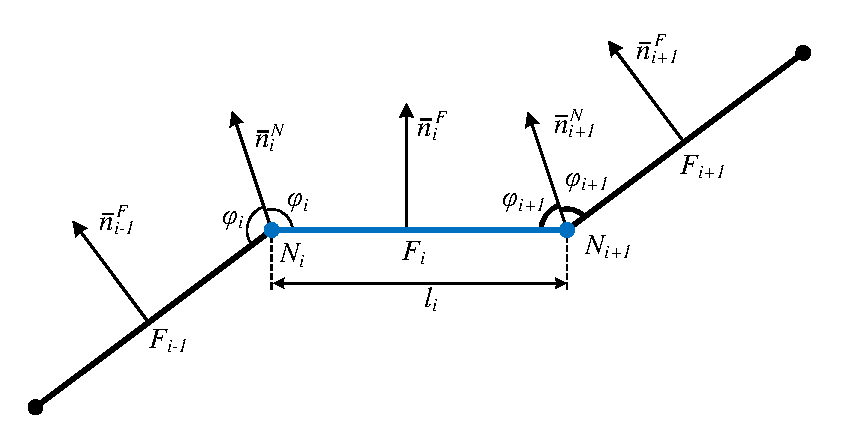
\includegraphics[width=0.75\columnwidth]{pics/text_1_remesh_2d/grid_normals.pdf}\caption{обозначения}\end{subfigure} &
\begin{subfigure}{0.45\textwidth}\centering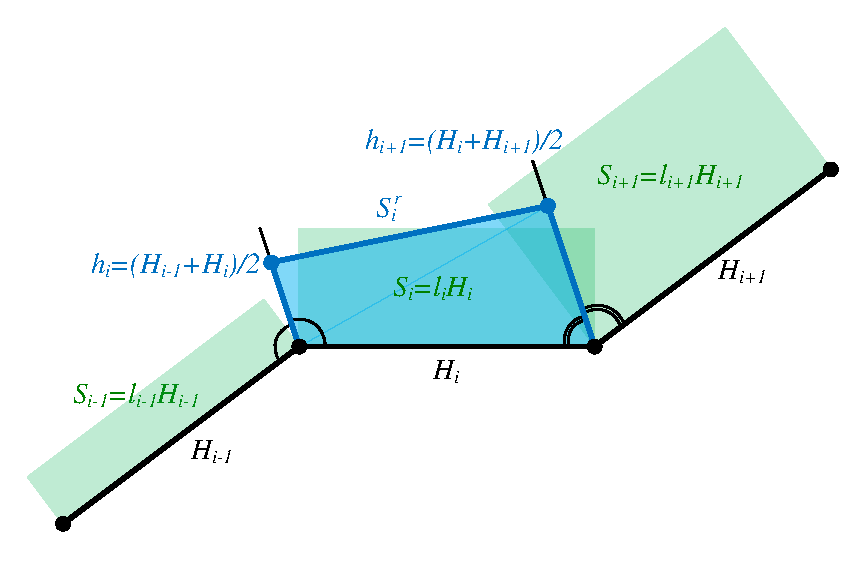
\includegraphics[width=0.75\columnwidth]{pics/text_1_remesh_2d/remesh_rectangles.pdf}\caption{метод прямоугольников}\end{subfigure} \\
\begin{subfigure}{0.45\textwidth}\centering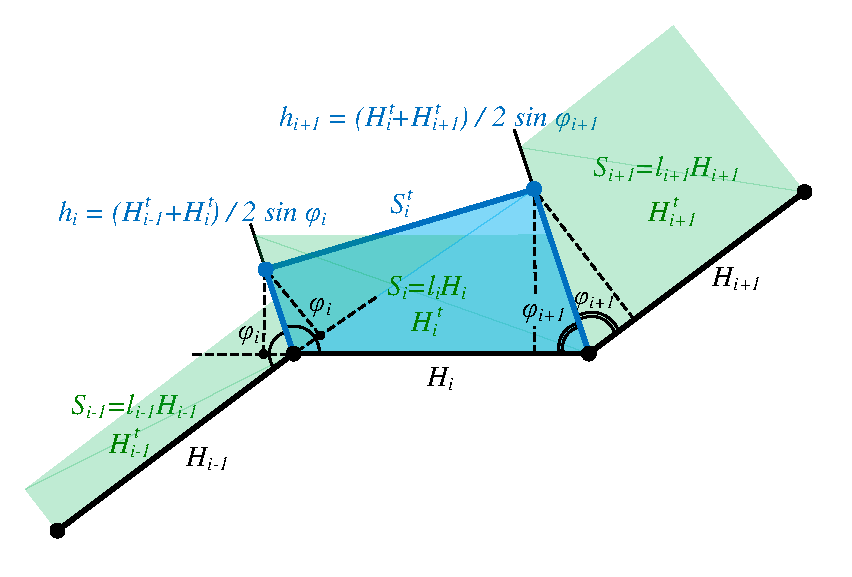
\includegraphics[width=0.75\columnwidth]{pics/text_1_remesh_2d/remesh_trapeziums.pdf}\caption{метод трапеций}\end{subfigure} &
\begin{subfigure}{0.45\textwidth}\centering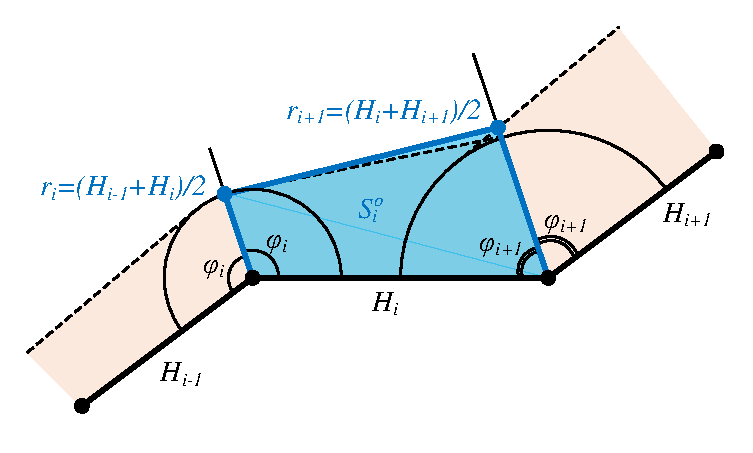
\includegraphics[width=0.75\columnwidth]{pics/text_1_remesh_2d/remesh_okrestnost.pdf}\caption{метод окрестностей}\end{subfigure}
\end{tabular}
\singlespacing
\caption{Перестроение двумерной поверхностной сетки.}
\label{fig:remesh_2d}
\end{figure}

Для моделирования процесса ледообразования центральной задачей перестроения поверхностной сетки является определение новых положений узлов $N'_i$, при которых площадь $S_i = S_{N_iN'_iN'_{i+1}N_{i+1}}$, заметаемая ячейкой $F_i$, как можно меньше отличалась от \textit{целевой площади} $T_i = l_i H_i$, где $H_i$ -- вычисленная высота ледяного покрова в ячейке $F_i$.
Задача рассматривается при фиксированных направлениях смещения узлов $\overline{n}_i^N$, то есть требуется определить только величины смещения узлов $h_i$.
Для оценки отклонения фактической заметаемой площади от целевой используются обозначения $\Delta_i = S_i - T_i$, $\delta_i = \Delta_i / T_i$.

%----------------------------------

В п.~1.1 задача определения величин смещений узлов $h_i$ рассматривается в общем виде, и она может быть решена с помощью метода градиентного спуска для нахождения минимума функции
\begin{equation*}
	D(\overline{h}) = \sum_{i = 0}^{n - 1}{\Delta_i^2} = \sum_{i = 0}^{n - 1}{ \left( \frac{ l_i(h_i \sin \phi_i + h_{i + 1} \sin \phi_{i+1}) - h_ih_{i + 1} \sin(\phi_i + \phi_{i+1}) }{2} - T_i \right)^2}
\end{equation*}

Так как решение задачи о перестроении сетки методом градиентного спуска оказывается слишком требовательным к вычислительным ресурсам, а также качество решения зачастую оказывается неудовлетворительным при попадании в локальные минимумы, то рассматриваются приближенные методы, основанные на представлении целевой площади в виде примитивных геометрических фигур.

%----------------------------------

В п.~1.2 рассматриваются приближенные методы перестроения поверхностной сетки.

В качестве первого метода рассматривается приближение, при котором целевая площадь для $i$-ой ячейки представлена прямоугольником со сторонами $l_i$ и $H_i$ и величина смещения определяется как $h_i = (H_{i - 1} + H_i)/2$ (рис.~\ref{fig:remesh_2d} b).
Этот метод перестроения поверхности будем называть \textit{методом прямогольников}.
Заметаемая $i$-ой ячейкой площадь при использовании метода прямоугольников обозначается $S_i^r$, также используются обозначения $\Delta_i^r = S_i^r - T_i$, $\delta_i^r = \Delta_i^r / T_i$.

В качестве второго метода рассматривается \textit{метод трапеций} (рис.~\ref{fig:remesh_2d} c).
В этом методе целевая площадь для $i$-ой ячейки представляется трапецией с площадью $T_i$ и боковыми сторонами, лежащими на направлениях $\overline{n}_i^N$, $\overline{n}_{i + 1}^N$, высота этой трапеции обозначена $H_i^t$.
После построения трапеций для всех ячеек сетки у каждого узла появляются две новые потенциальные позиции для сдвига (образованные ячейкой слева и ячейкой справа).
В качестве финальной новой позиции выбирается их среднее значение, и $h_i = (H_{i - 1}^t + H_i^t) / (2 \sin \phi_i)$.
Заметаемая $i$-ой ячейкой площадь при использовании метода трапеций обозначается $S_i^t$, также используются обозначения $\Delta_i^t = S_i^t - T_i$, $\delta_i^t = \Delta_i^t / T_i$.

Предлагается новый метод перестроения, называемый \textit{методом окрестностей}.
В этом методе рассматривается \textit{область распространения льда (ОРЛ)} и сетки (рис.~\ref{fig:remesh_2d} d).
При этом ОРЛ узла $N_i$ считается круг с центром $N_i$ и радиусом $r_i = (H_{i - 1} + H_i)/2$.
Под ОРЛ ячейки понимается выпуклая оболочка ОРЛ ее узлов и ограниченная ей область плоскости.
Тогда ОРЛ сетки является объединение ОРЛ ее ячеек.
В качестве нового положения узла $N_i$ берется пересечение направления $\overline{n}_i^N$ и границы ОРЛ сетки.
Заметаемая $i$-ой ячейкой площадь при использовании метода окрестностей обозначается $S_i^o$, также используются обозначения $\Delta_i^o = S_i^o - T_i$, $\delta_i^o = \Delta_i^o / T_i$.

%----------------------------------

В п.~1.3 приводится аналитическая оценка точности приближенных методов перестроения.
Оценка проводится для модельной расчетной сетки, которая удовлетворяет следующим требованиям.
Все ячейки сетки одинаковые и имеют длину $l$.
Для любой ячейки $AB$ и ее соседей $A_2A$ и $BB_2$ углы $\angle (\overline{BA}, \overline{AA_2})$ и $\angle (\overline{AB}, \overline{BB_2})$ являются постоянной величиной и равны $\alpha$.
Величины смещений ячеек $A_2A$, $AB$ и $BB_2$ равны $H_{i - 1}$, $H_i$ и $H_{i + 1}$ соответственно.
Величины смещения узлов равны $h_i = AA_1$, $h_{i + 1} = BB_1$, также $\lambda = l / (2 \sin \frac{\alpha}{2})$.
Оценка проводится для постоянного изменения смещения ячейки $\Delta H = H_i - H_{i - 1} = H_{i + 1} - H_i$.

\begin{figure}[ht]
\centering
\begin{tabular}{cc}
\begin{subfigure}{0.4\textwidth}\centering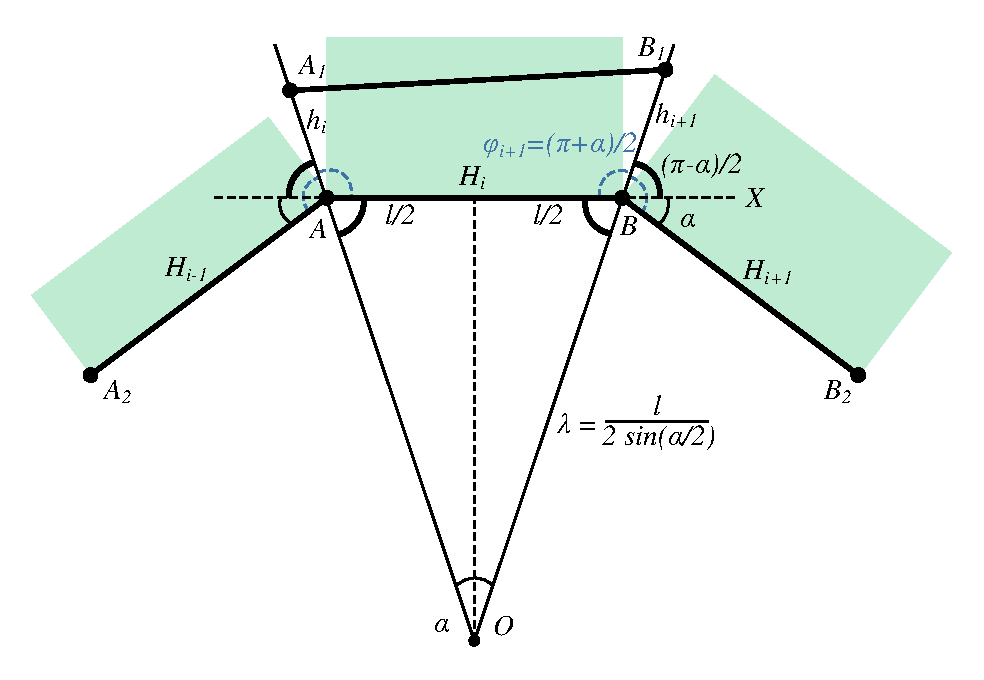
\includegraphics[width=1.0\columnwidth]{pics/text_1_remesh_2d/theoretical.pdf}\caption{выпуклая сетка}\end{subfigure} &
\begin{subfigure}{0.4\textwidth}\centering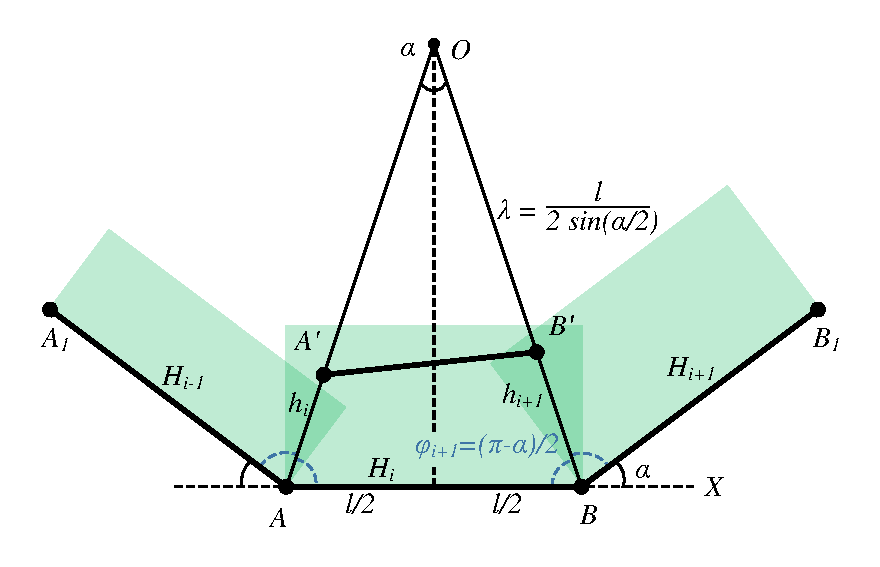
\includegraphics[width=1.0\columnwidth]{pics/text_1_remesh_2d/theoretical_concave.pdf}\caption{вогнутая сетка}\end{subfigure}
\end{tabular}
\singlespacing
\caption{Оценка точности перестроения приближенных методов.}
\label{fig:remesh_2d_accuracy}
\end{figure}

Для выпуклой и вогнутой сеток в обозначенных условиях приводятся следующие утверждения для вычисления заметаемой площади.

\textbf{Лемма.} \textit{Для ячейки выпуклой сетки $S_i = \frac{1}{2} \sin \alpha \left( \lambda(h_i + h_{i+1}) + h_ih_{i+1} \right)$ (рис.~\ref{fig:remesh_2d_accuracy} a).}

\textbf{Лемма.} \textit{Для ячейки вогнутой сетки $S_i = \frac{1}{2} \sin \alpha \left( \lambda(h_i + h_{i+1}) - h_ih_{i+1} \right)$ при выполнении условия $\max(h_i, h_{i+1}) \le \lambda$ (рис.~\ref{fig:remesh_2d_accuracy} b).}

\begin{figure}[ht]
\centering
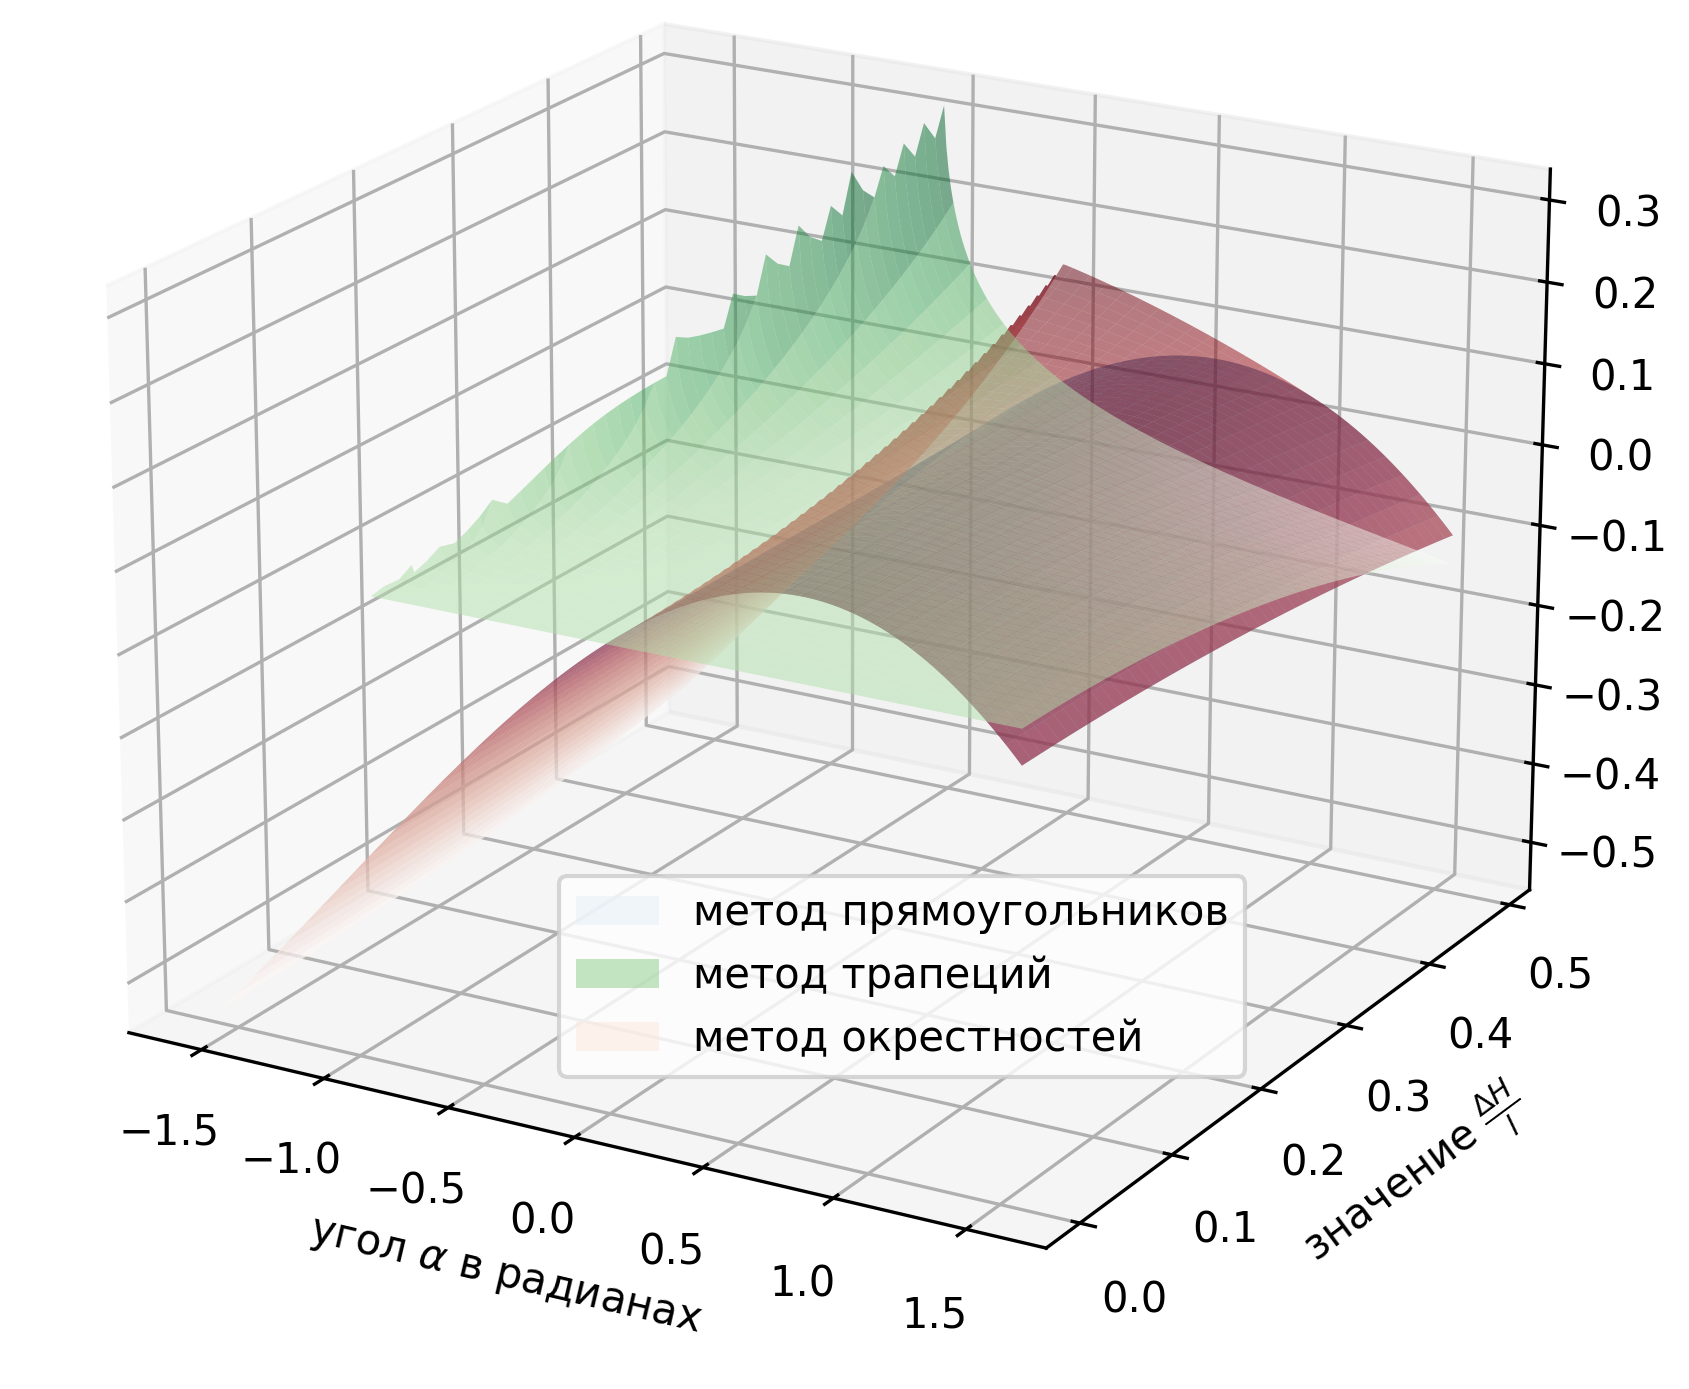
\includegraphics[width=0.45\textwidth]{pics/text_1_remesh_2d/remesh_3d_chart.png}
\singlespacing
\caption{Графики $\delta_i^r(\alpha, \frac{\Delta H}{l})$, $\delta_i^t(\alpha, \frac{\Delta H}{l})$, $\delta_i^o(\alpha, \frac{\Delta H}{l})$ при $H = \frac{l}{2}$.}
\label{fig:text_1_remesh_3d_main_chart}
\end{figure}

Исходя из утверждений формулу $S_i = \frac{1}{2} \sin \alpha \left( \lambda(h_i + h_{i+1}) + h_ih_{i+1} \right)$ можно использовать как для выпуклой сетки, так и для вогнутой (приняв $\alpha < 0$).

Для трех рассмотренных методов перестроения получены выражения для $h_i$ в аналитическом виде, получены зависимости $\delta_i^r(\alpha, \frac{\Delta H}{l})$, $\delta_i^t(\alpha, \frac{\Delta H}{l})$, $\delta_i^o(\alpha, \frac{\Delta H}{l})$ и проведен их анализ, представленный на рис.~\ref{fig:text_1_remesh_3d_main_chart} и рис.~\ref{fig:text_1_remesh_fix_alfa_chart}.

Из рис.~\ref{fig:text_1_remesh_3d_main_chart} можно отметить, что при $\Delta H = 0$ метод трапеций абсолютно точен.
Также при $\Delta H = 0$ отклонения $\delta_i^r$ и $\delta_i^o$ близки.

\begin{figure}[ht]
\centering
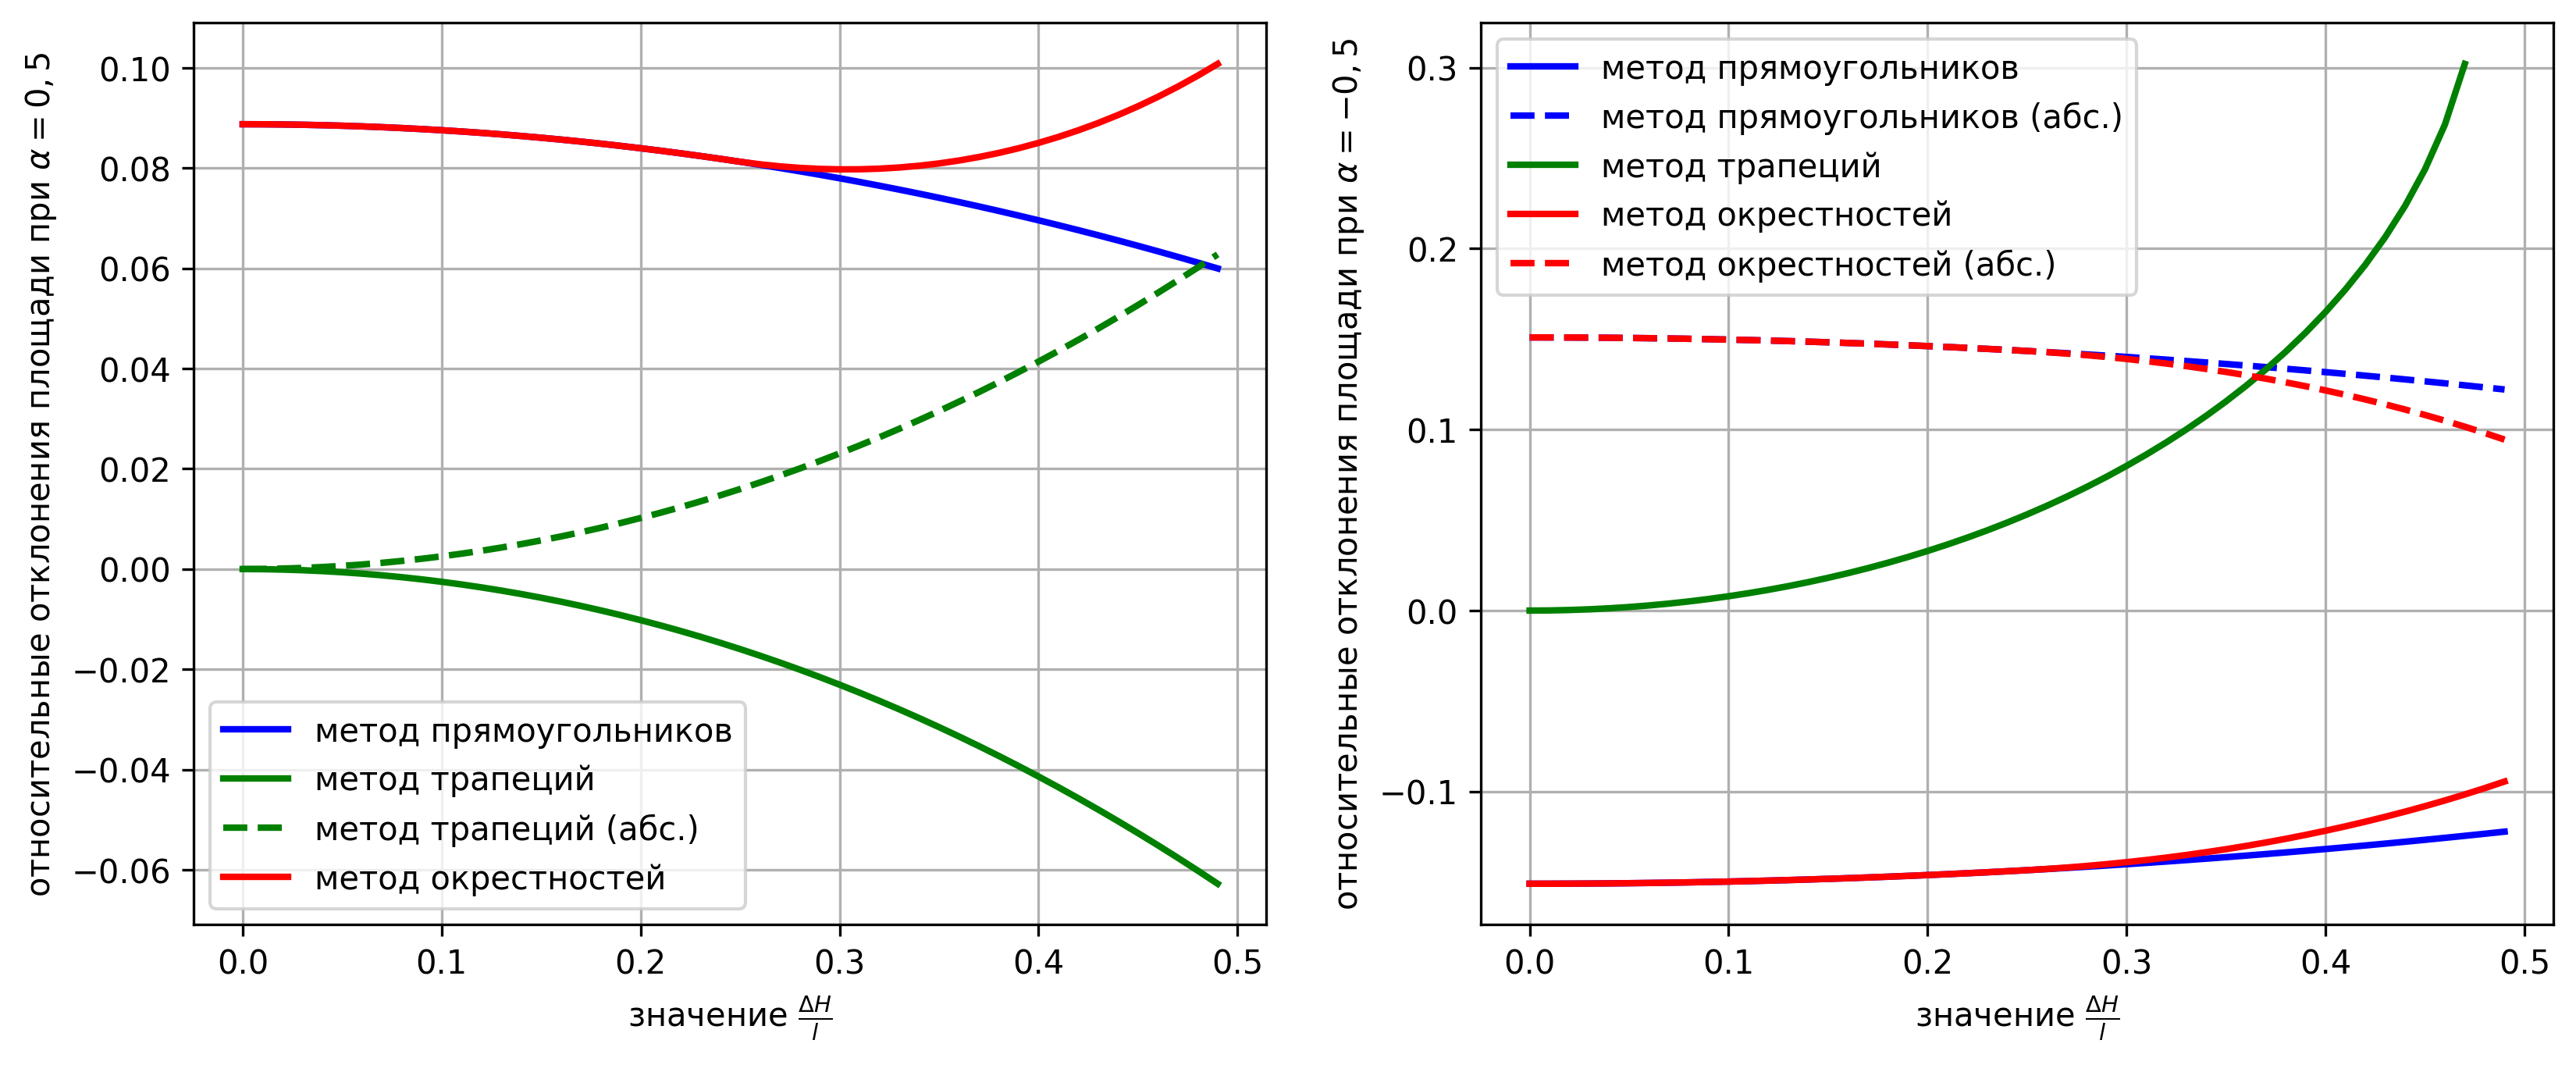
\includegraphics[width=0.8\textwidth]{pics/text_1_remesh_2d/remesh_fix_alfa_chart.png}
\singlespacing
\caption{Графики поверхностнй $\delta_i^r(\frac{\Delta H}{l})$, $\delta_i^t(\frac{\Delta H}{l})$, $\delta_i^o(\frac{\Delta H}{l})$ при $\alpha = \pm 0,5$.}
\label{fig:text_1_remesh_fix_alfa_chart}
\end{figure}

Дополнительно приводятся зависимости $\delta_i^r$, $\delta_i^t$, $\delta_i^o$ от $\frac{\Delta H}{l}$ при фиксированных значениях $\alpha = \pm 0,5$ (рис.~\ref{fig:text_1_remesh_fix_alfa_chart}).
Из рисунка видно, что метод трапеций при небольших значениях $\frac{\Delta H}{l}$ наиболее точен, а точность методов прямоугольников и окрестностей достаточно близки.

%----------------------------------

В п.~1.4 приведены оценки сглаживания острых пиков и впадин для рассмотренных методов перестроения сетки (методы прямоугольников, трапеций и окрестностей).
Для этого рассматривается расчетная сетка с одинаковыми ячейками-отрезками длины $l$.

Для оценки сглаживания острых пиков считается, что сетка является абсолютно плоской за исключением двух соседних ячеек, которые образуют острый пик с углом $2 \alpha$.
Аналогично для оценки сглаживания впадин считается, что сетка является абсолютно плоской за исключением двух соседних ячеек, которые образуют впадину с углом $2 \alpha$ (рис.~\ref{fig:text_1_remesh_2d_peak_cavern_general}).

В описанных услових и обозначениях сформулированы утверждения.

\begin{figure}[ht]
\centering
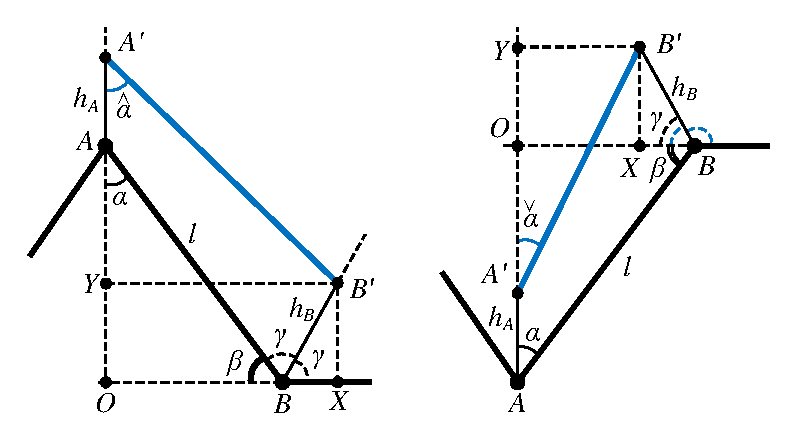
\includegraphics[width=0.6\textwidth]{./pics/text_1_remesh_2d/peak-cavern-general.pdf}
\singlespacing
\caption{Оценка сглаживания угла при остром пике и при впадине.}
\label{fig:text_1_remesh_2d_peak_cavern_general}
\end{figure}

\textbf{Лемма.} \textit{Сглаженный угол при остром пике выражается как $\hat{\alpha}_1(h_A, h_B) = \arctg \frac{l \sin \alpha + h_B \cos \gamma}{l \cos \alpha + h_A - h_B \sin \gamma}$ (рис.~\ref{fig:text_1_remesh_2d_peak_cavern_general} слева).}

\textbf{Лемма.} \textit{Сглаженный угол при впадине выражается как $\check{\alpha}_1(h_A, h_B) = \arctg \frac{l \sin \alpha - h_B \cos \gamma}{l \cos \alpha - h_A + h_B \sin \gamma}$ при условии $\arcsin \frac{h_B \left( \sqrt{8 l^2 + h_B^2} - h_B \right)}{4 l^2} \le \alpha \le \arccos \frac{h_A}{l}$ (рис.~\ref{fig:text_1_remesh_2d_peak_cavern_general} справа).}

\begin{figure}[ht]
\centering
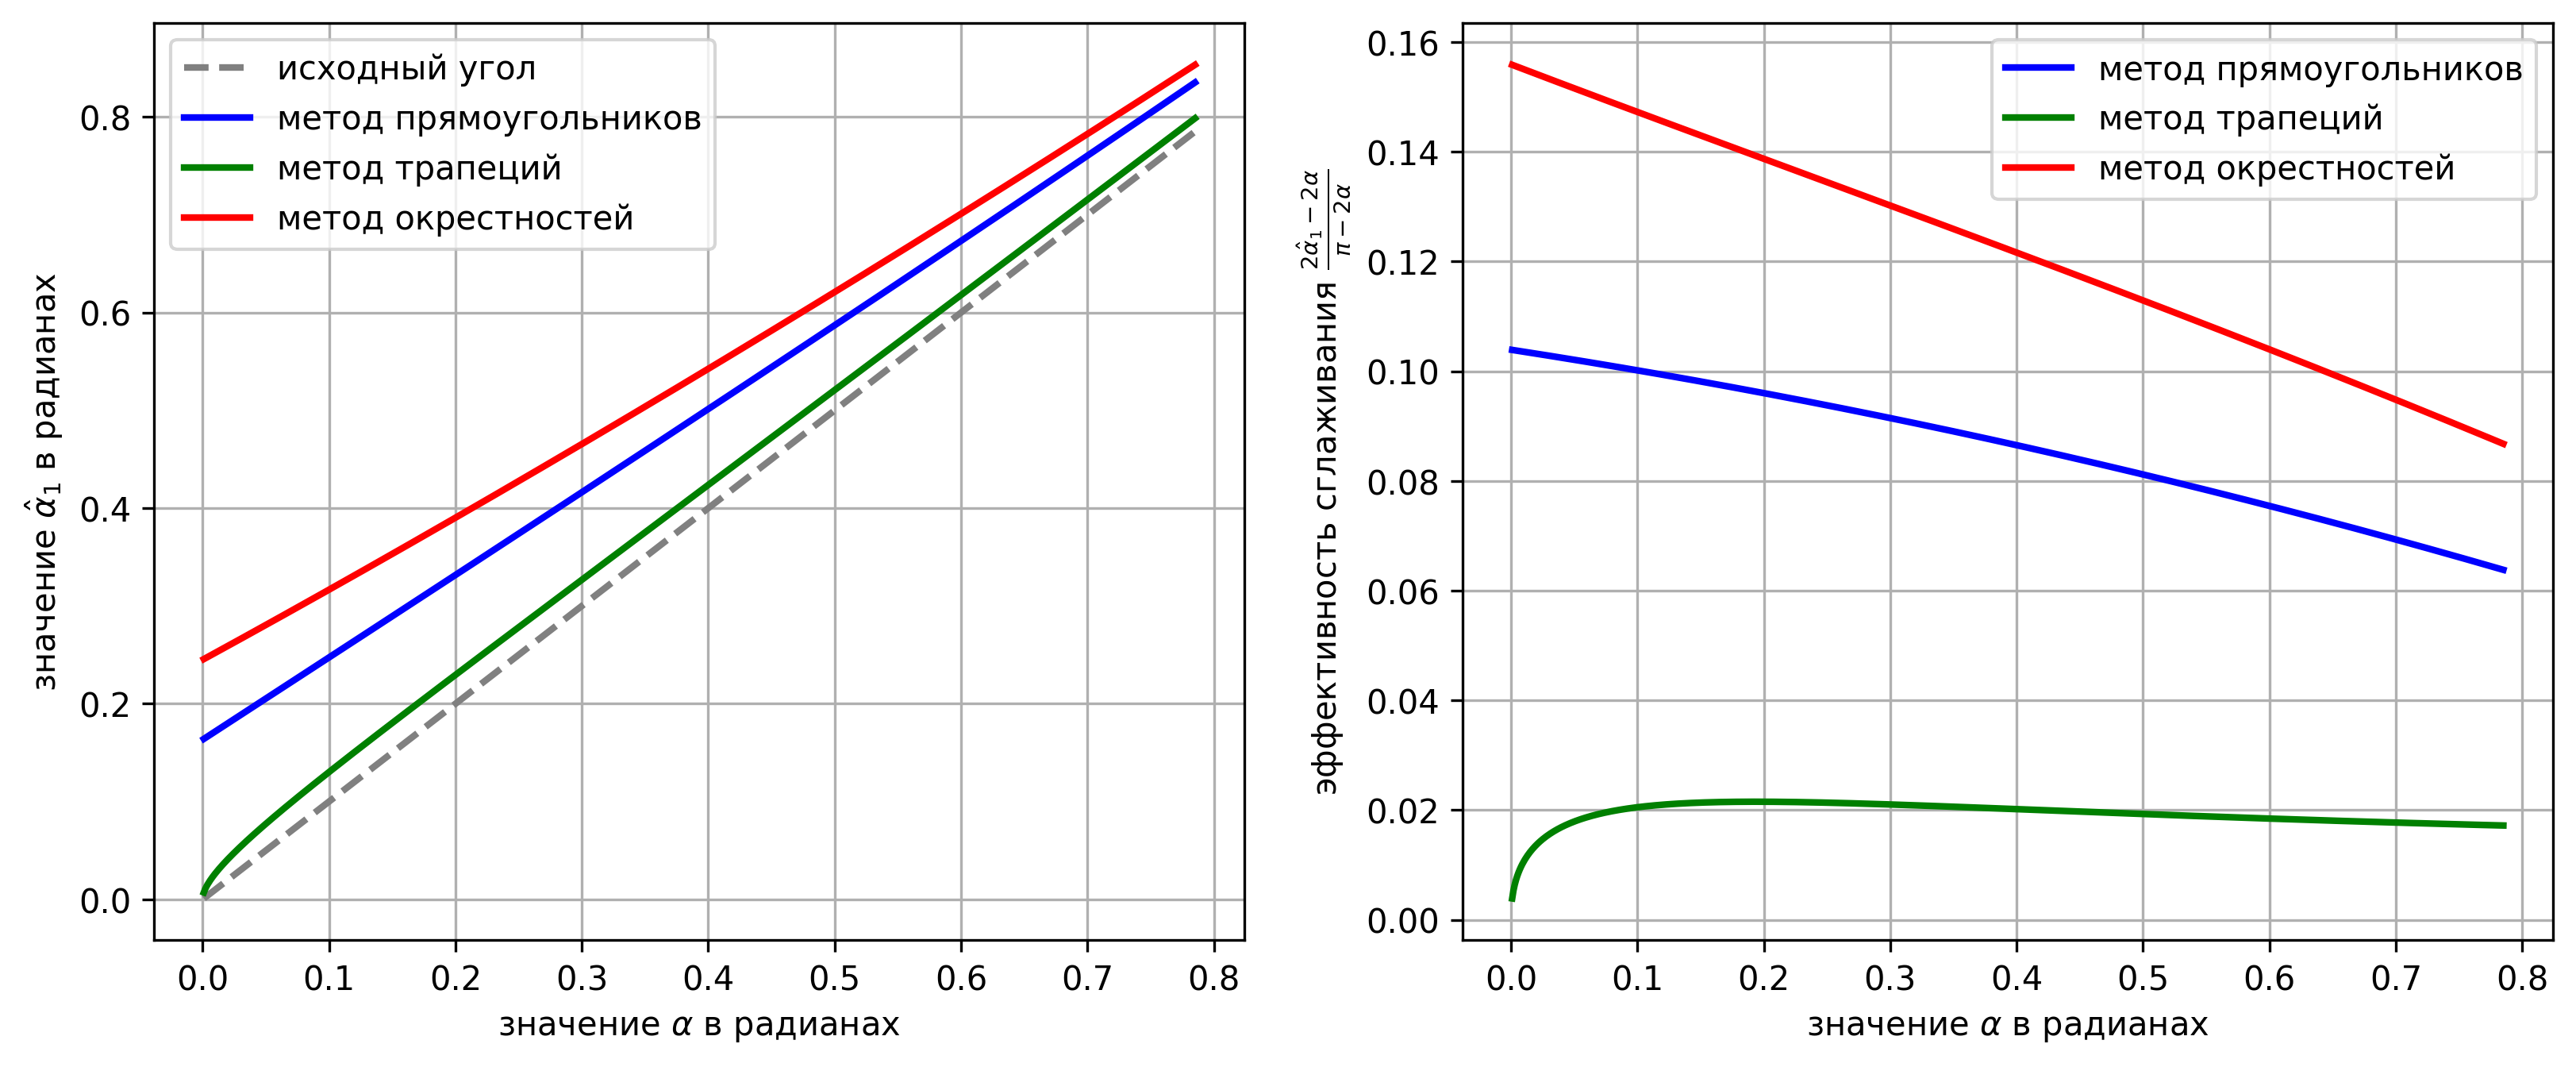
\includegraphics[width=0.8\textwidth]{./pics/text_1_remesh_2d/peak-methods-chart.png}
\singlespacing
\caption{Сравнение сглаживания угла при остром пике.}
\label{fig:text_1_remesh_2d_peak_methods_chart}
\end{figure}

\begin{figure}[!ht]
\centering
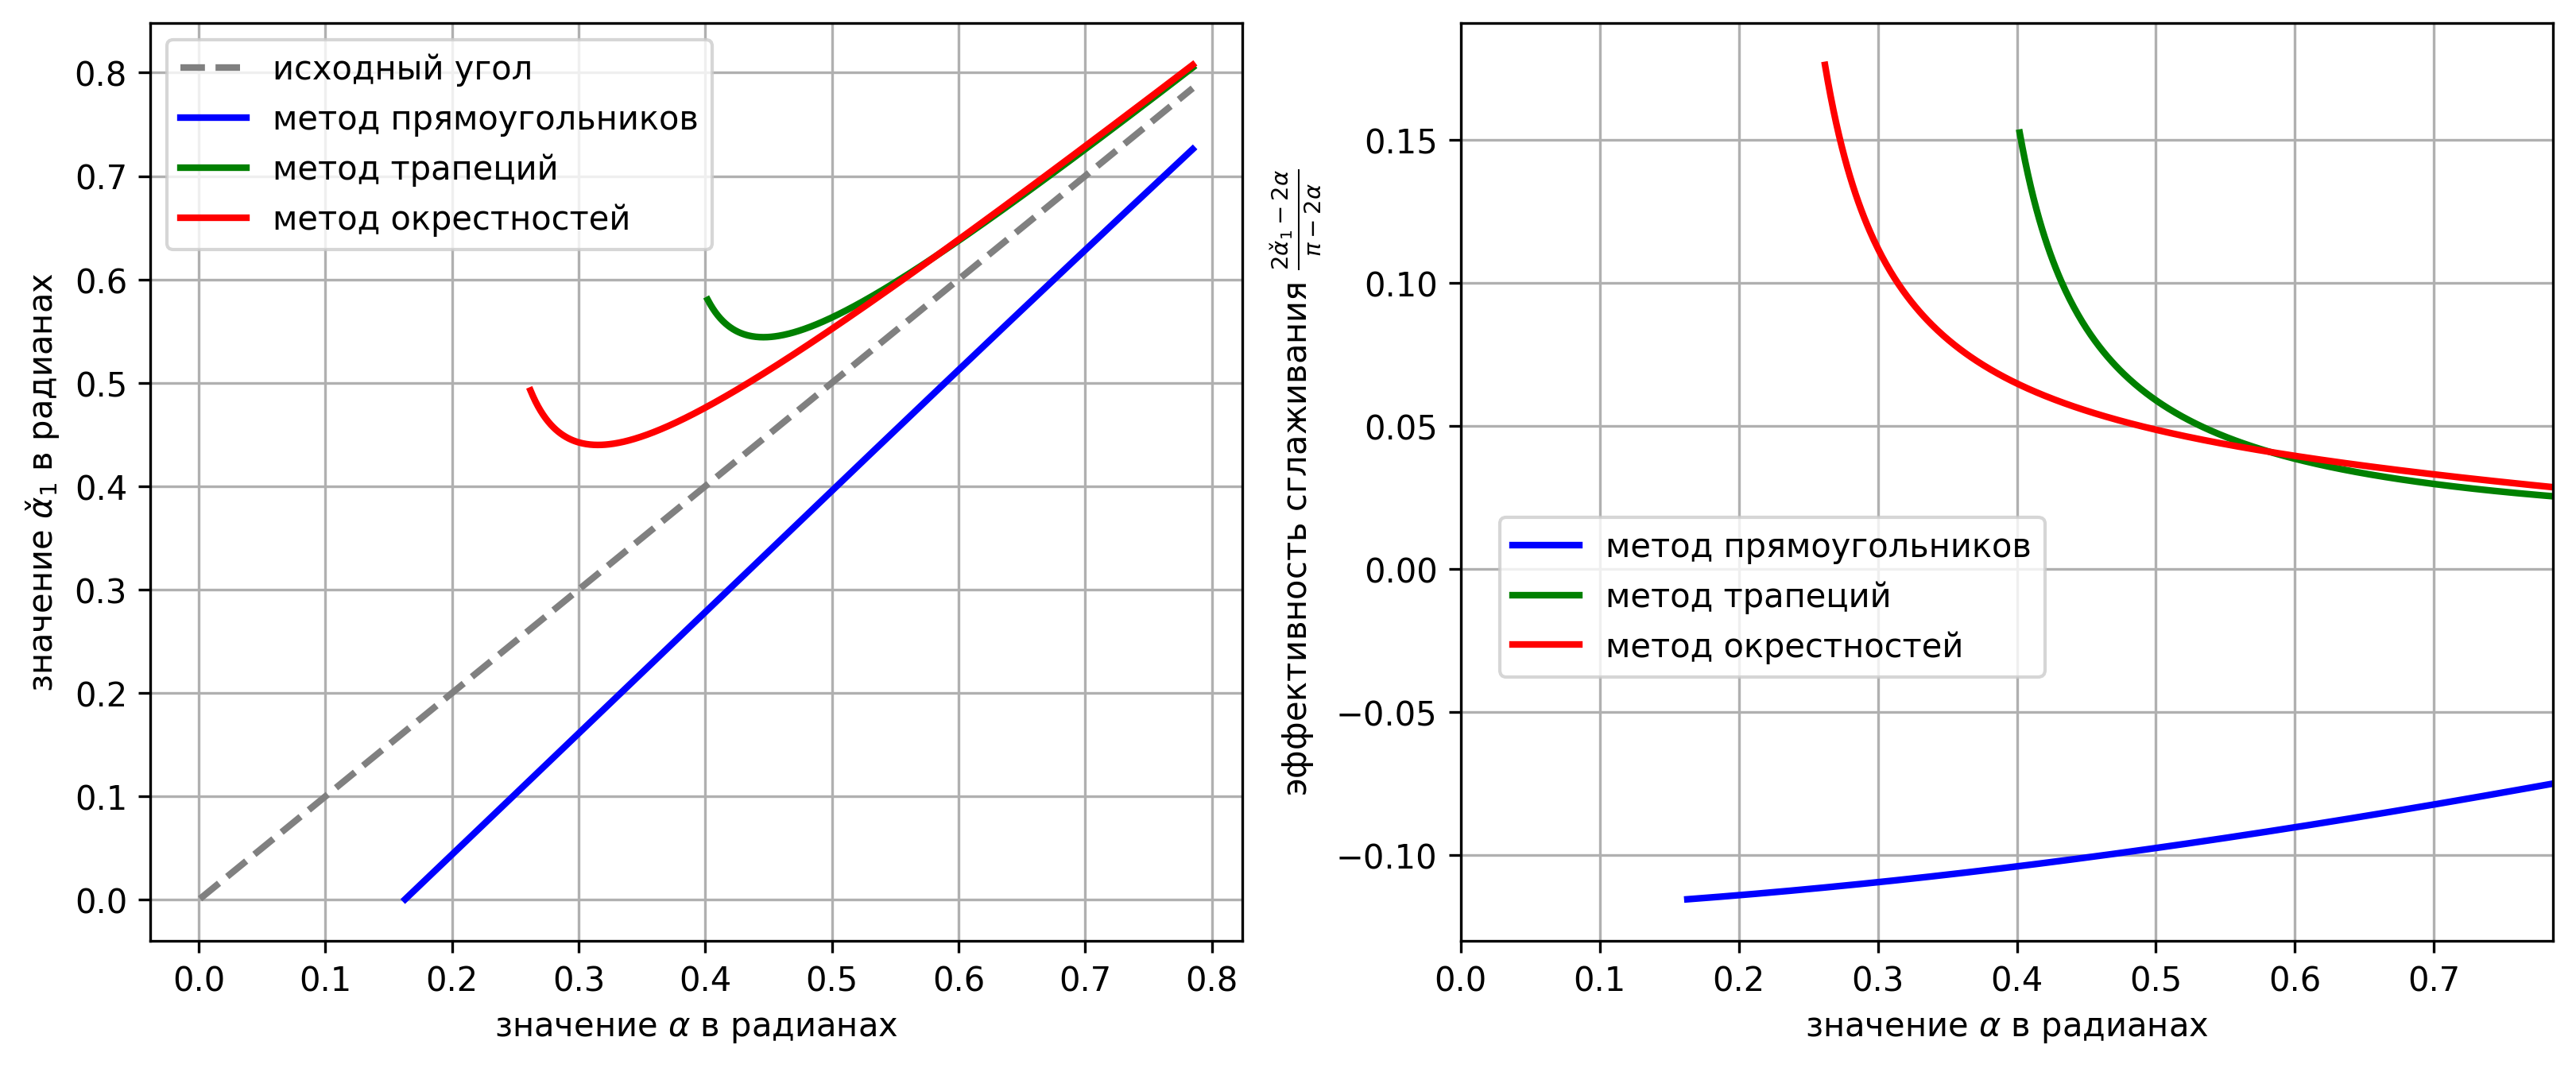
\includegraphics[width=0.8\textwidth]{./pics/text_1_remesh_2d/cavern-methods-chart.png}
\singlespacing
\caption{Сравнение сглаживания угла при впадине.}
\label{fig:text_1_remesh_2d_cavern_methods_chart}
\end{figure}

На рис.~\ref{fig:text_1_remesh_2d_peak_methods_chart} приведены графики сравнения методов перестроения в применении к сглаживанию острых пиков при $H = \frac{l}{4}$.
На графике слева показана зависимость изменения сглаженного угла $\hat{\alpha}_1$ от $\alpha$.
На графике справа показана эффективность сглаживания, выраженная формулой $\frac{2 \hat{\alpha}_1 - 2 \alpha}{\pi - 2 \alpha}$ (значение 1 означает полное сглаживание пика до угла $\hat{\alpha}_1 = \frac{\pi}{2}$).
Наиболее эффективное сглаживание угла $\alpha$ обеспечивает метод окрестностей.
Также, использование метода трапеций для малых углов $\alpha$ приводит к неконтролируемому росту $h_A$, что делает применение этого метода неприемлемым.

На рис.~\ref{fig:text_1_remesh_2d_cavern_methods_chart} приведены графики сравнения методов перестрения в применении к сглаживанию впадин при $H = \frac{l}{4}$.
На графике слева показана зависимость изменения сглаженного угла $\check{\alpha}_1$ от $\alpha$.
На графике справа показана эффективность сглаживания, выраженная формулой $\frac{2 \check{\alpha}_1 - 2 \alpha}{\pi - 2 \alpha}$ (значение 1 означает полное сглаживание пика до угла $\hat{\alpha}_1 = \frac{\pi}{2}$).
Отметим, что метод прямоугольников не сглаживает угол, а наоборот, делает его еще более острым (значение эффективности сглаживания меньше нуля).
Метод трапеций показывает лучшую эффективность сглаживания, но с меньшей областью применимости.

Из приведенных оценок на рис.~\ref{fig:text_1_remesh_2d_peak_methods_chart} и рис.~\ref{fig:text_1_remesh_2d_cavern_methods_chart} можно сделать вывод, что метод окрестностей перестроения является оптимальным с точки зрения точноси перестроения и способности сглаживания дефектов сетки.

%---------------------------------------------------------------------------------------------------

\textbf{Вторая глава} посвящена задаче перестроения поверхностной сетки в трехмерном случае.

Рассматривается трехмерная поверхностная неструктурированная сетка с треугольными ячейками.
Для каждой ячейки $F$ определена внешняя единичная нормаль $\overline{n}_F^F$.
Единичная нормаль для узла определяется аналогично двумерному случаю $\overline{n}_N^N = \sum_{F \in \mathscr{F}(N)}{\overline{n}_F^F} / |\sum_{F \in \mathscr{F}(N)}{\overline{n}^F(F)}|$, где $\mathscr{F}(N)$ -- множество ячеек, инцидентных $N$.

%----------------------------------

В п.~2.1 рассматривается постановка задачи перестроения поверхностной неструктурированной расчетной сетки в трехмерном случае при фиксированных направлениях смещения узлов, совпадающих с $\overline{n}^N(N)$.
Задача рассматривается в постановке, когда в каждой ячейке сетки известен объем накопленного льда ($V_F$).
Для каждого узла сетки $N$ требуется найти его новое положение в пространстве $N'$, чтобы для каждой ячейки с узлами $ABC$ объем пространства, ограниченный фигурой $ABCA'B'C'$ соответствовал объему льда, накопленному в этой ячейке.
Таким образом, поставновка задачи в трехмерном случае аналогично двумерной постановке.

\begin{figure}[h]
\centering
\begin{tabular}{ll}
\begin{subfigure}{0.4\textwidth}\centering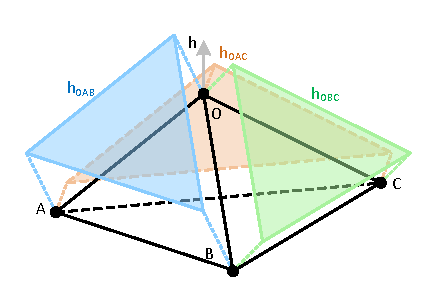
\includegraphics[width=1.0\columnwidth]{pics/text_1_remesh_3d/pic_classical_methods_prisms.pdf}\caption{метод призм}\end{subfigure} &
\begin{subfigure}{0.45\textwidth}\centering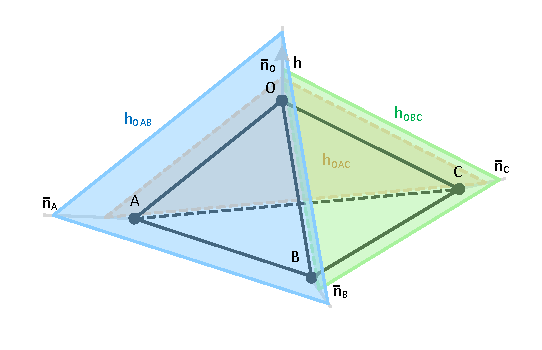
\includegraphics[width=1.0\columnwidth]{pics/text_1_remesh_3d/pic_classical_methods_pyramids.pdf}\caption{метод пирамид}\end{subfigure}
\end{tabular}
\singlespacing
\caption{Перестроение поверхностной сетки с трехмерном случае.}
\label{fig:text_1_remesh3}
\end{figure}

Для трехмерной постановки рассматриваются классические приближенные методы перестроения, аналогичные двумерному случаю (рис.~\ref{fig:text_1_remesh3}).
В \textit{методе призм} перестроения поверхности (аналог метода прямоугольников в двумерной постановке) в качестве приближения заметаемого объема рассматривается призма, одним из оснований которой является ячейка.
В \textit{методе пирамид} перестроения поверхности (аналог метода трапеций в двумерной постановке) в качестве приближения заметаемого объема рассматривается призматоид, одним из оснований которого является ячейка, в боковые стороны направлены вдоль направлений смещения узлов.

Также рассматриваются дополнительные вопросы перестроения поверхностной сетки.
В частности многослойный метод перестроения, в котором выполнятеся $k$ последовательных шагов перестроения сетки, на каждом из которых решается задача для объема накопленного в ячейке $F$ льда в количестве $V_F/k$.
Рассматриваются метод сглаживания поля нормалей для предотвращения раннего самопересечения сетки, метод сглаживания высот для устранения поверхностного шума, а также метод сглаживания сетки, позволяющий перераспределить узлы по поверхности для балансировки размера ячеек. 

%----------------------------------

В п.~2.2 предлагается метод окрестностей перестроения поверхностной неструктурированной расчетной сетки в трехмерной постановке.
Рассмотривается геометрическая задача определения новых положений узлов расчетной сетки, если для каждого узла $N$ известна скорость образования ледяного покрова $v_N$.
Будем считать, что нарастание льда в любой точке роста льда выполняется одновременно во всех направлениях аналогично принципу Гюйгенса-Френеля распространения волн.
Таким образом, ОРЛ произвольной точки $P$ через промежуток времени $\Delta t$ будет иметь форму шара $Ball(P, v_P\Delta t)$.
Далее будем считать, что мы выполняем расчет новых положений узлов через некоторый фиксированный момент времени $\Delta t$, то есть для каждого узла $N$ известен радиус ОРЛ узла $R_N = v_N \Delta t$.
Радиус ОРЛ внутренней точки ячейки сетки будем определять как $R(P(\beta,\gamma)) = R(\beta,\gamma) = R_A + \beta(R_B - R_A) + \gamma(R_C - R_A)$.
Тогда ОРЛ ячейки является объединение пучка шаров $Ball(P(\beta, \gamma), R(\beta, \gamma))$ для $\beta \ge 0$, $\gamma \ge 0$, $\beta + \gamma \le 1$.

\begin{figure}[!ht]
\centering
\begin{tabular}{ll}
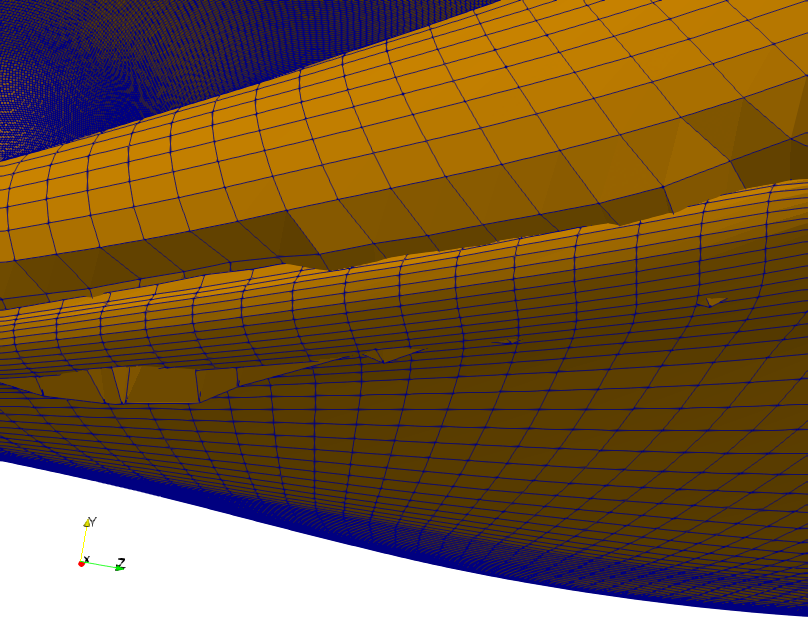
\includegraphics[width=0.45\textwidth]{pics/text_1_remesh_3d/fens1.png}
&
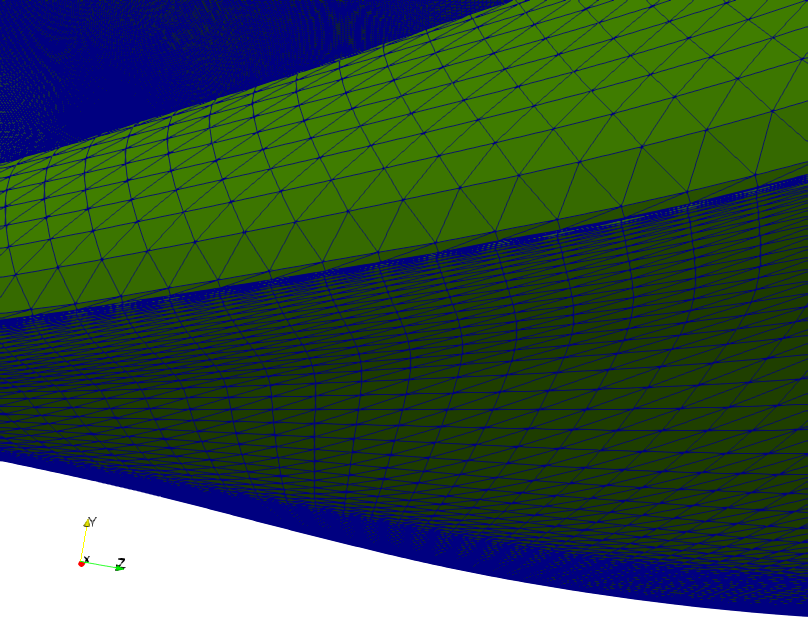
\includegraphics[width=0.45\textwidth]{pics/text_1_remesh_3d/crys1.png} \\
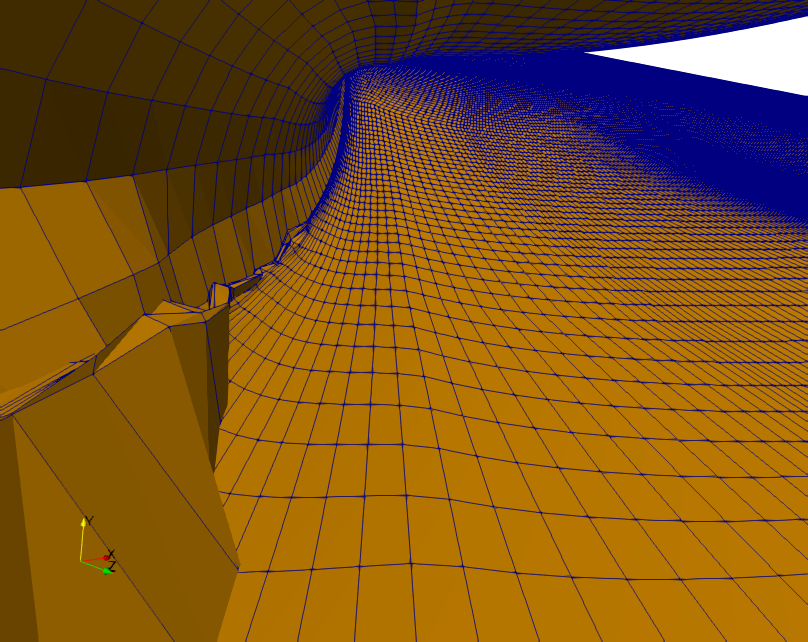
\includegraphics[width=0.45\textwidth]{pics/text_1_remesh_3d/fens2.png}
&
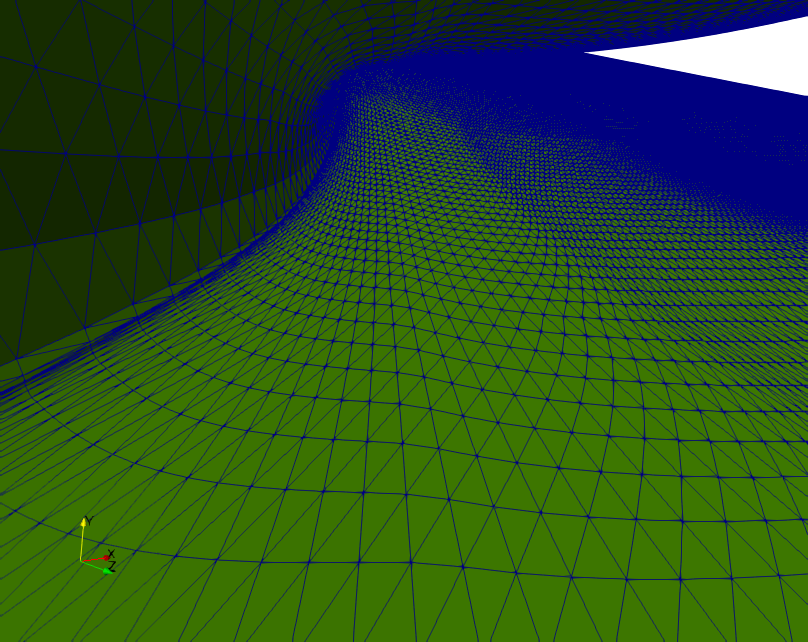
\includegraphics[width=0.45\textwidth]{pics/text_1_remesh_3d/crys2.png}
\end{tabular}
\singlespacing
\caption{Эффект сглаживания дефектов при перестроении методом окрестностей (справа) в сравнении с программным комплексом FENSAP.}
\label{fig:text_1_remesh3_with_fensap}
\end{figure}

Рассматривается задача нахождения точек пересечения траектории движения узла ячейки $A$ ($\overline{P}(\alpha) = \overline{A} + \alpha \overline{D}$ при $\alpha \ge 0$) с фронтом продвижения ячейки.
Эти точки находятся из решения уравния $|(\overline{A} + \alpha \overline{D}) - \overline{C}(\beta, \gamma)| = R(\beta, \gamma)$ относительно $\alpha$.

\textbf{Лемма.} \textit{Наибольший корень уравнения $|(\overline{A} + \alpha \overline{D}) - \overline{C}(\beta, \gamma)| = R(\beta, \gamma)$ при условии $|\overline{D}| = 1$ выражается следующим образом:
\begin{equation*}
	\begin{aligned}
		& \alpha(\beta, \gamma) = k_{\beta} \beta + k_{\gamma} \gamma + \sqrt{T} \\
		& T = q_{\beta^2} \beta^2 + q_{\gamma^2} \gamma^2 + q_{\beta \gamma} \beta \gamma + q_{\beta} \beta + q_{\gamma} \gamma + q \\
		& k_{\beta} = (\overline{D}, \overline{AB}), \ k_{\gamma} = (\overline{D}, \overline{AC}) \\
		& q_{\beta^2} = (\overline{D}, \overline{AB})^2 - |\overline{AB}|^2 + R_{AB}^2, \ q_{\gamma^2} = (\overline{D}, \overline{AC})^2 - |\overline{AC}|^2 + R_{AC}^2 \\
		& q_{\beta \gamma} = 2 \left( (\overline{D}, \overline{AB}) (\overline{D}, \overline{AC}) - (\overline{AB}, \overline{AC}) + R_{AB}R_{AC} \right) \\
		& q_{\beta} = 2 R_A R_{AB}, \ q_{\gamma} = 2 R_A R_{AC}, \ q = R_A^2
	\end{aligned}
\end{equation*}}
где $R_{AB} = R_B - R_A$, $R_{AC} = R_C - R_A$.

Требуемая точка пересечения соответствует максимальному значению $\alpha(\beta, \gamma)$ при ограничениях $\beta \ge 0$, $\gamma \ge 0$, $\beta + \gamma \le 1$.
Изложенная последовательность действий касается определения смещения узла с учетом только одной инцидентной ячейки.
При рассмотрении отдельного узла расчетной сетки требуется вычислить смещение этого узла относительно каждой инцидентной ячейки и выбрать среди этих смещений максимальное.

Предложенный метод окрестностей перестроения поверхностной неструктурированной расчетной сетки в трехмерном случае, также как и его двумерный аналог, обладает способностью сглаживания дефектов расчетной сетки при приемлемой точности перестроения (рис.~\ref{fig:text_1_remesh3_with_fensap}).

%---------------------------------------------------------------------------------------------------

\textbf{Третья глава} посвящена проблемам нахождения пересечений неструктурированной поверхностной сетки с другими расчетными сетками.

В п.~3.1 рассматривается проблема устранения самопересечений поверхностной неструктурированной расчетной сетки.
Самопересечение является критическим дефектом сетки, при котором невозможно производить дальнейшие вычисления по моделированию ледообразования, поэтому самопересечения необходимо удалять.
В общем случае предотвратить самопересечение невозможно, так как в процессе ледообразования при активном нарастании льда возможно переречение одних ледяных наростов с другими ледяными наростами.
Таким образом, для адекватного моделирования процесса ледообразования необходимо уметь корректно обрабатывать самопересечения расчетной сетки, чтобы после возникновения самопересечения можно быть продолжать выполнение расчетов.

\begin{figure}[!ht]
\centering
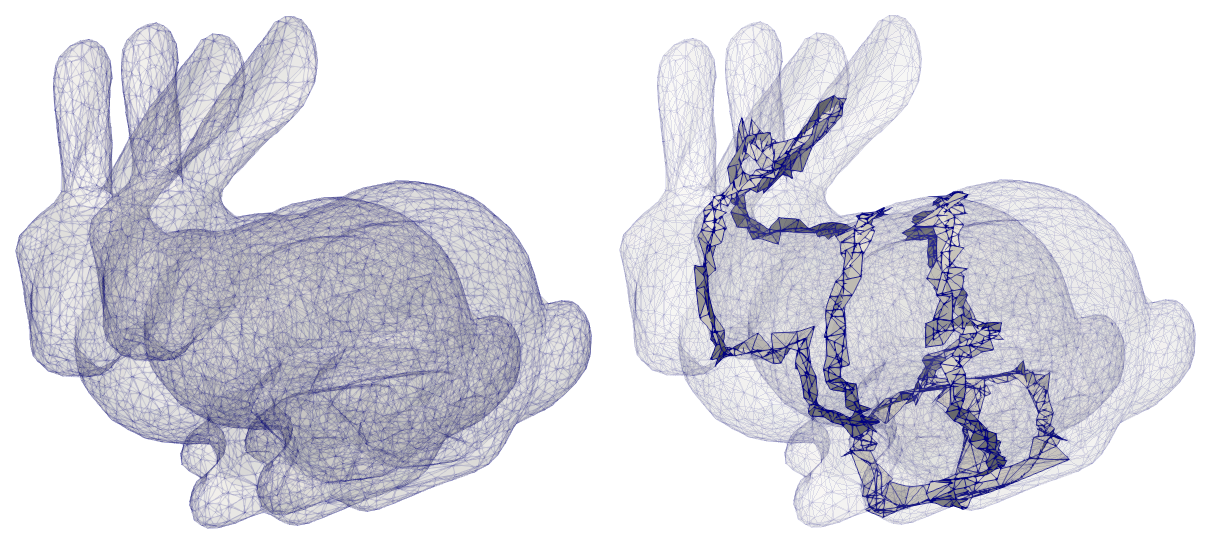
\includegraphics[width=1.0\textwidth]{./pics/text_1_int/bunnies_dbl.png}
\singlespacing
\caption{Устранение самопересечений в случае достаточной точности определения пересечения пар треугольников.}
\label{fig:text_1_int_1}
\end{figure}

Предлагаются два подхода к устранению самопересечений.
Сначала требуется найти всех пары пересекающихся ячеек сетки.
Для этого используется иерархическая структура дерева треугольников, позволяющая избежать проверки на пересечение каждой пары ячеек.
Основной проблемой при поиске пересечений двух треугольников являются ошибки точности, из-за которых может быть принято ошибочное решение о пересечении: попадание узла сетки на ребро или на ячейку, пересечение двух ребер сетки, пересечение ячеек под острым углом.
В некоторых случаях такие конфликты можно разрешить локальной коррекцией положения узлов.
Если конфликты удается разрешить, и все пары пересекающися ячеек определены корректно, то все пересекающиеся ячейки сетки разбиваются на более мелкие ячейки по всем точкам пересечения, после чего внешняя часть сетки определяется путем обхода ячеек (рис.~\ref{fig:text_1_int_1}).

\begin{figure}[!ht]
\centering
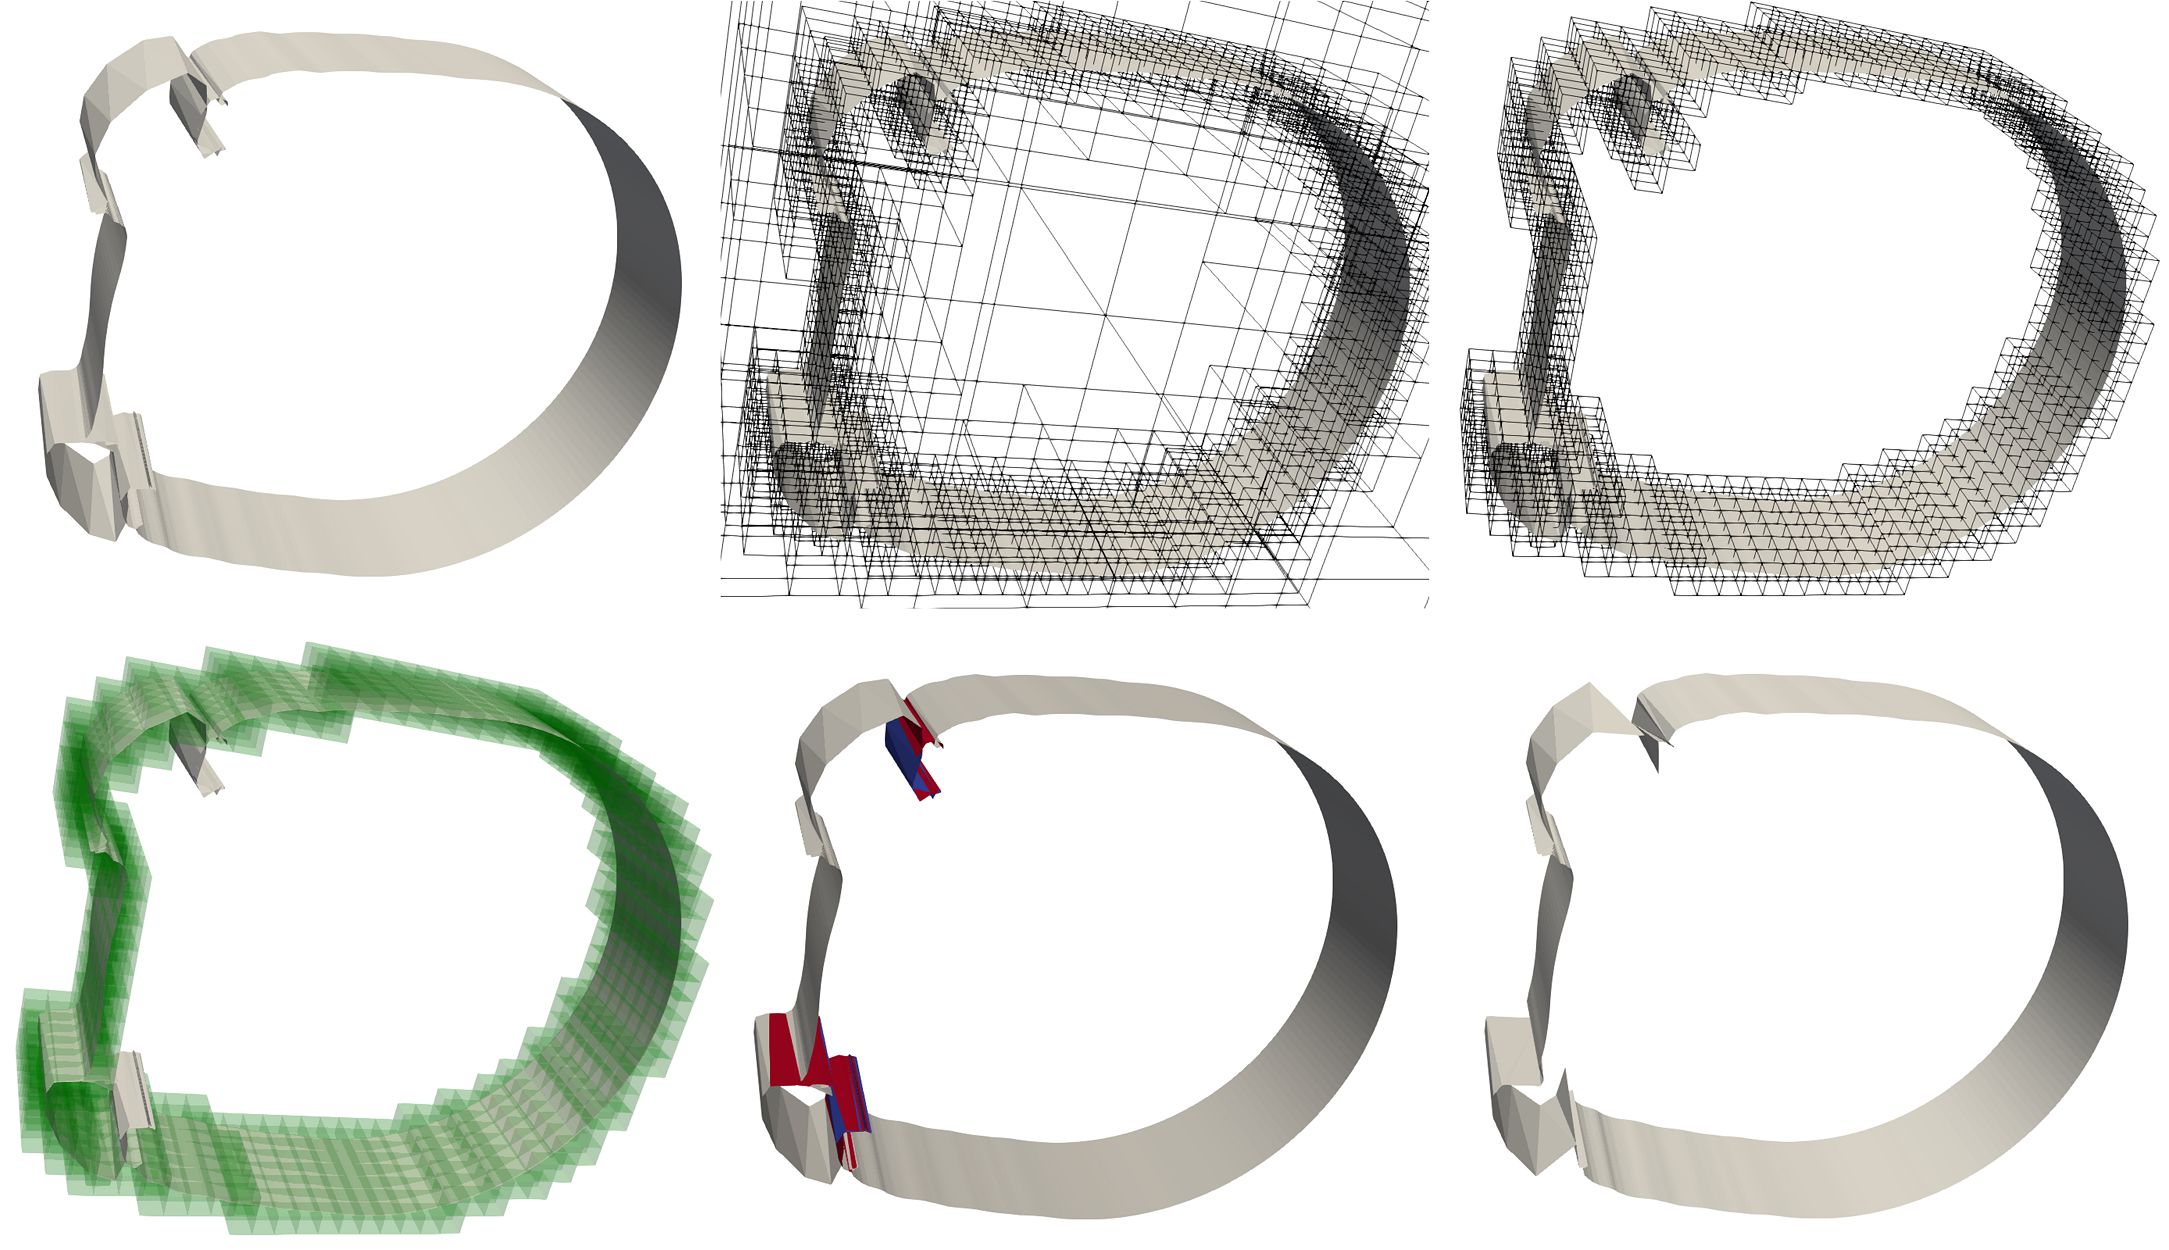
\includegraphics[width=1.0\textwidth]{./pics/text_1_int/wing_all.png}
\singlespacing
\caption{Устранение самопересечения с использованием подложки поверхностной сетки.}
\label{fig:text_1_int_2}
\end{figure}

При перестроении поверхности для задачи ледообразования расчетная сетка, как правило, отличается низким качеством -- в ней могут присутствовать ячейки с углами, близкими к $0$ или $\pi$, что препятствует корректному определению точек пересечения.
В этом случае используется второй подход к устранению самопересечений.
В пространстве строится восьмеричное дерево вложенных кубов, называемое \textit{подложкой}, где корень охватывает всю поверхность, а дочерние кубы строятся только в случае пересечения с сеткой.
Минимальный размер ячейки подложки выбирается меньше минимального ребра поверхностной сетки.
Далее определяется внешний слой кроны подложки, и все ячейки, не пересекающие этот слой, помечаются как кандидаты на удаление из сетки.
Также помечаются все ячейки, пересекающие другие ячейки в сетке.
После чего выполняется шаг стягивания сетки по ребрам, входящим в помеченную область.
После этого процесс повторяется итерационно, пока расчетная сетка не будет избавлена от самопересечений.
Такой подход не гарантирует устранение самопересечений, однако в отдельных случаях он оказывается применимым (например для расчетов на псевдотрехмерных профилях, рис.~\ref{fig:text_1_int_2}).

%----------------------------------

В п.~3.2 рассматривается проблема сопряжения поверхностной сетки с объемной сеткой для определения поля скоростей вокруг обтекаемого тела.
При расчете обледенения крайне важным элементом данных является поле скоростей в области, окружающей рассматриваемую поверхность.
Поле скоростей вблизи поверхности влияет на движение жидкой пленки по поверхности, что существенным образом определяет картину обледенения.
Также при использовании модели вторичного увлажнения отскочившие от поверхности капли попадают в свободный поток, и поле скоростей необходимо для расчета траектории их движения и зоны вторичного выпадения.
Так как при перестроении поверхностной сетки построение согласованной объемной сетки является затратной процедурой, то для возможности продолжения расчетов предлагается метод погруженной границы с фиктивными ячейками.

Для реализации метода погруженной границы также используется подложка поверхностной расчетной сетки, и в этом разделе более детально рассматривается вопрос поиска пересечений поверхностной сетки с подложкой.
Для поиска пересечений поверхностной сетки с подложкой используется представление треугольной ячейки в виде ГМТ $P(\beta, \gamma) = A + \beta (B - A) + \gamma (C - a), \beta \ge 0, \gamma \ge 0, \beta + \gamma \le 1$ и ячейки в форме прямоугольного параллелепипеда в виде ГМТ $x_l \le x_P \le x_h, y_l \le y_P \le y_h, z_l \le z_P \le z_h$ и поиска точек, входящий в оба ГМТ методов свертывания системы линейных неравенств.

%----------------------------------

В п.~3.3 рассматривается \textit{метод погруженной границы} с использованием \textit{фиктивных ячеек} в трехмерной постановке.
В предлагаемом методе строится подложка поверхностной сетки, в которой ячейки кроны подложки разделяются на три категории ячеек 
Внешними ячейками будем называть те ячейки, которые целиком лежат вне тела.
Внутренние ячейки лежат целиком внутри тела, все остальные ячейки пересекают границу тела и являются граничными.
В методе погруженной границы с использованием фиктивных ячеек из граничных ячеек выделяются ячейки, для которых меньшая часть объема находится вне тела, а большая -- внутри тела.
Такие ячейки называются фиктивными.
Это разделение ячеек на классы является первичным и весьма приближенным, так как после коррекции некоторые внутренние ячейки могут быть также переведены в разряд фиктивных (в процессе проведения вычислений должно выполняться следующее требование: соседями внутренних ячеек не могут являться ни граничные, ни внешние ячейки).
На каждой итерации расчетов для фиктивных ячеек требуется выполнить аппроксимацию газодинамических величин (плотность, давление, вектор скорости), чтобы эти фиктивные ячейки могли быть использованы для определения потоков между ними и соседними с ними граничными и внешними ячейками.
Аппроксимация скалярных и векторных газодинамических величин в фиктивных ячейками выполняется с помощью шаблонов, в которые входят три внешние ячейки, а также точка поверхности, в которой известно направление нормали.

%---------------------------------------------------------------------------------------------------

\textbf{Четвертая глава} посвящена вопросам распараллеливания вычислений на расчетных сетках.

%----------------------------------

В п.~4.1 приводятся основные показатели качества декомпозиции расчетной сетки при распределении ячеек по \textit{доменам}.

В качестве первого показателя качества декомпозиции сетки (\textit{неравномерность декомпозиции}) принимается максимальное абсолютное отклонение размера домена от теоретически возможного среднего значения $D = \max_{1 \le i \le k}{ \left( n_i - \frac{n}{k} \right) }$, где $n_i$ – количество ячеек в $i$-ом домене.
Наряду с ним используются показатели $D^{*} = \frac{D}{n / k}$ и $D^{\%} = D^{*} \cdot 100\%$.

В качестве второй характеристики качества декомпозиции будем использовать величину наиболее протяженной границы между парой доменов, или $L_{ij} = \left| \{ e \in E: \{ d(e_a), d(e_b) \} = \{ i, j \} \} \right|$, $L = \max_{1 \le i < j \le k}{L_{ij}}$, где $d(с)$ -- домен, к которому относится $с$.
Наряду с показателем $L$ используется нормированный показатель $L^{*}$, определяемый как $L^{*} = \frac{L}{|E|}$, а также $L^{\%} = L^{*} \cdot 100\%$.

В роли дополнительной характеристики качества декомпозиции можно использовать суммарную длину границ между доменами $I = \sum_{1 \le i < j \le k}{L_{ij}}$, что соответствует общему количеству пересылаемых данных в рамках межпроцессного обмена (аналогичные показатели $I^{*} = \frac{I}{|E|}$ и $I^{\%} = I^{*} \cdot 100\%$).

%----------------------------------

В п.~4.2 рассматривается проблема распределения вычислительной нагрузки при проведении вычислений на блочно-структурированной расчетной сетке между узлами вычислительного кластера.

Рассматривается архитектура блочно-структурированной расчетной сетки с поддержкой дробления блоков, приводится иерархия входящих в ее состав элементов, а также описывается механизм организации межпроцессных обменов.

Сначала рассматривается задача распределения вычислительной нагрузки без дробления.
Рассмотрим множество $X$ вещественных чисел $x_i \ge 0$ для $i \in N$, где $N = [1, n]$.
Рассмотрим также множество индексов $j \in M$, где $M = [1, m]$.
Будем говорить, что определено разбиение множества $X$ на $m$ множеств, если введена функция $\gamma(i): N \rightarrow M$.
Множество всех функций разбиения будем обозначать $\Gamma(N, M)$.
Веса результирующих множеств будем определять естественным образом для $j \in M$: $X_j = \sum_{\substack{i \in N \\ \gamma(i) = j}}{x_i}$.
Требуется найти такую функцию разбиения $\gamma \in \Gamma(N, M)$, чтобы минимизировать наиболее тяжелое из результирующих множеств $\max_{j \in M}{X_j}$.

Точное решение поставленное задачи может быть найдено с помощью метода ветвей и границ (TODO - описание алгоритма).

Рассмотрим жадный алгоритм решения этой задачи.
В жадном алгоритме будем последовательно обрабатывать все веса, начиная с наибольшего.
Каждый необработанный вес будем относить к наиболее легкому на текущий момент множеству весов.

Тогда верно следующее утверждение.

\textbf{Лемма}. \textit{При использовании жадного алгоритма распределения весов между отдельными множествами отклонение наиболее тяжелого множества $\max_{j \in M}{X_j}$ от среднего значения веса множеств $\langle X \rangle$ не превышает максимальный остаточный член $r_i$, то есть $\max_{j \in M}{X_j} - \langle X \rangle \le \max_{i \in N}{r_i}$, где $r_i = \max{\left( x_i - \frac{1}{m} \sum_{p = i}^{n}{x_p}, 0 \right)}$.}

TODO - сравнение точного и жадного алгоритма (Монте-Карло).

Рассмотрим различные стратегии дробления блоков при недостижении допустимого отклонения $D^{\%}$ при распределении блоков по процессам.

Простейшая стратегия дробления блоков описывается следующим образом.
Сначала нужно применить жадный алгоритм распределения весов блоков по вычислительным узлам.
Если требуемое отклонение $D^{\%}$ наибольшего веса вычислительного узла от среднего значения достигнуто, то можно завершать работу.
В противном случае нужно разделить максимальный блок пополам по наиболее протяженному направлению, после чего произвести перераспределение.
Этот жадный алгоритм с дроблением пополам будем обозначать UG (от uniform greedy).
Этот алгоритм всегда завершает работу, однако в отдельных случаях может выполнять необоснованно большое количество дроблений блоков, что приводит к увеличению объема межпроцессных обменов в процессе счета.

Для устранения крупных блоков без лишних дроблений предлагается механизм минимизации количества разрезов блоков, обозначаемый MCC (от minimal cuts count).

\begin{figure}[!ht]
\centering
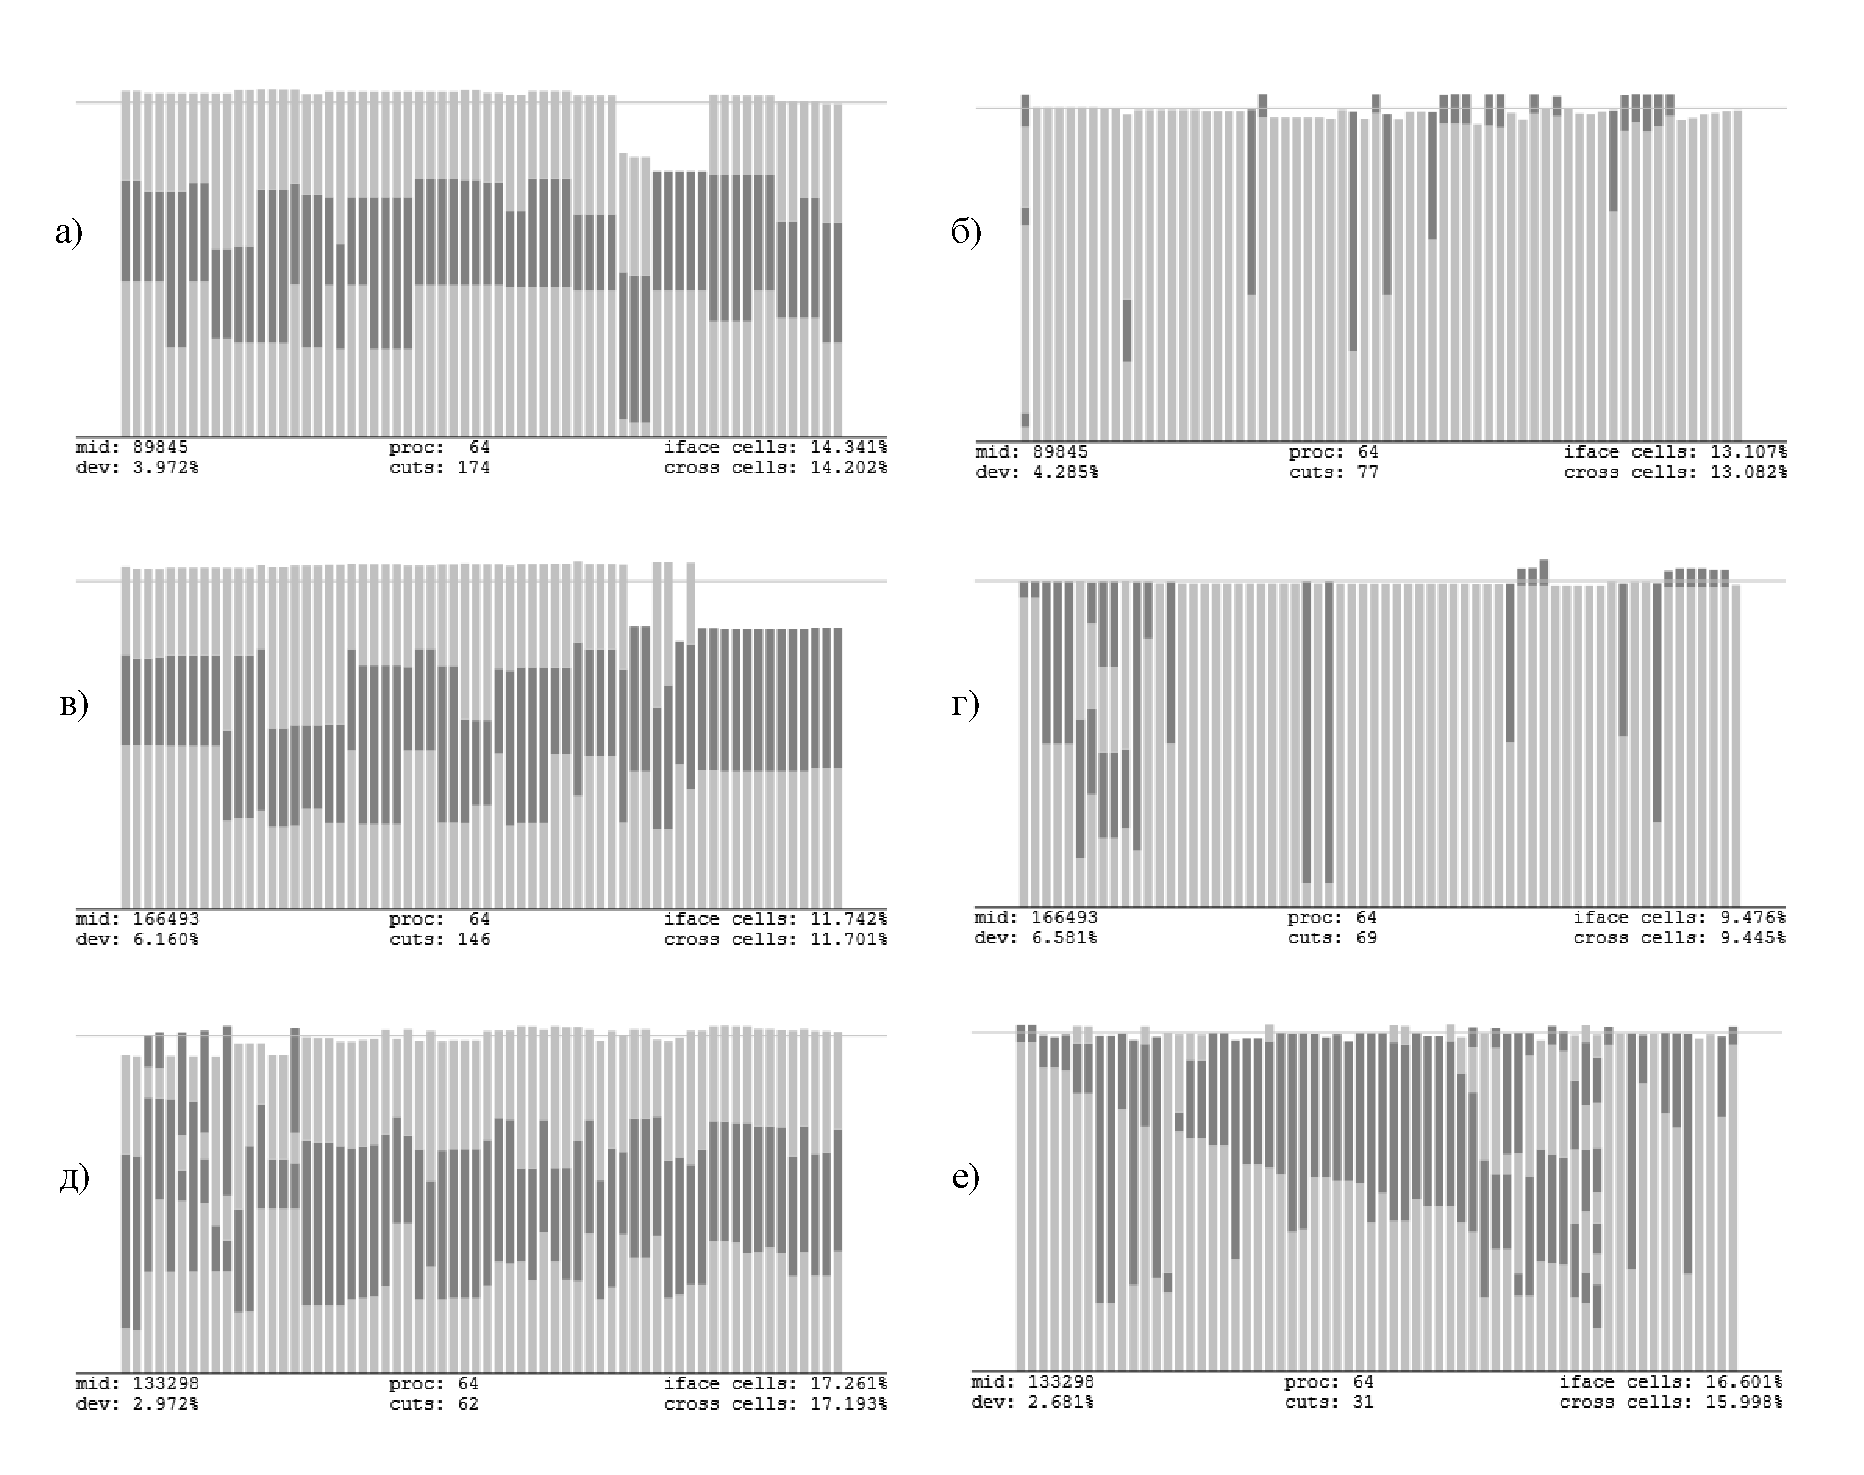
\includegraphics[width=1.0\textwidth]{./pics/text_2_withcut/2-merged-pic.pdf}
\singlespacing
\caption{Гистограммы распределения блоков расчетной сетки по вычислительным узлам суперкомпьютера для сеток test (а, б), train (в, г), ref (д, е) с помощью алгоритмов UG (а, в, д) и MCC (б, г. е).}
\label{fig:text_2_withcut_2_merged_pic}
\end{figure}

Результаты сравнения эффективности методов UG и MCC распределения вычислительной нагрузки между узлами суперкомпьютера показывают, что использование метода MCC оправдано, так как с его помощью можно добиться распределения не худшего качества (а зачастую и лучшего), чем при использовании UG.
При этом MCC позволяет существенно сократить количество разрезов блоков сетки для достижения требуемого результата.
Также использование MCC приводит к сокращению количества MPI ячеек в сетке, что положительно сказывается на скорости межпроцессных обменов данными.
Особенно явно достоинства метода MCC проявляются на сетках с относительно небольшим количеством блоков и наличием ярко выраженных крупных блоков.

Приводятся результаты эксперимента по выполнению расчетов на блочно-структурированной расчетной сетке с дроблением максимального блока для достижения различных значений допустимой неравномерности распределения $D^{\%}$.

\begin{figure}[ht]
\centering
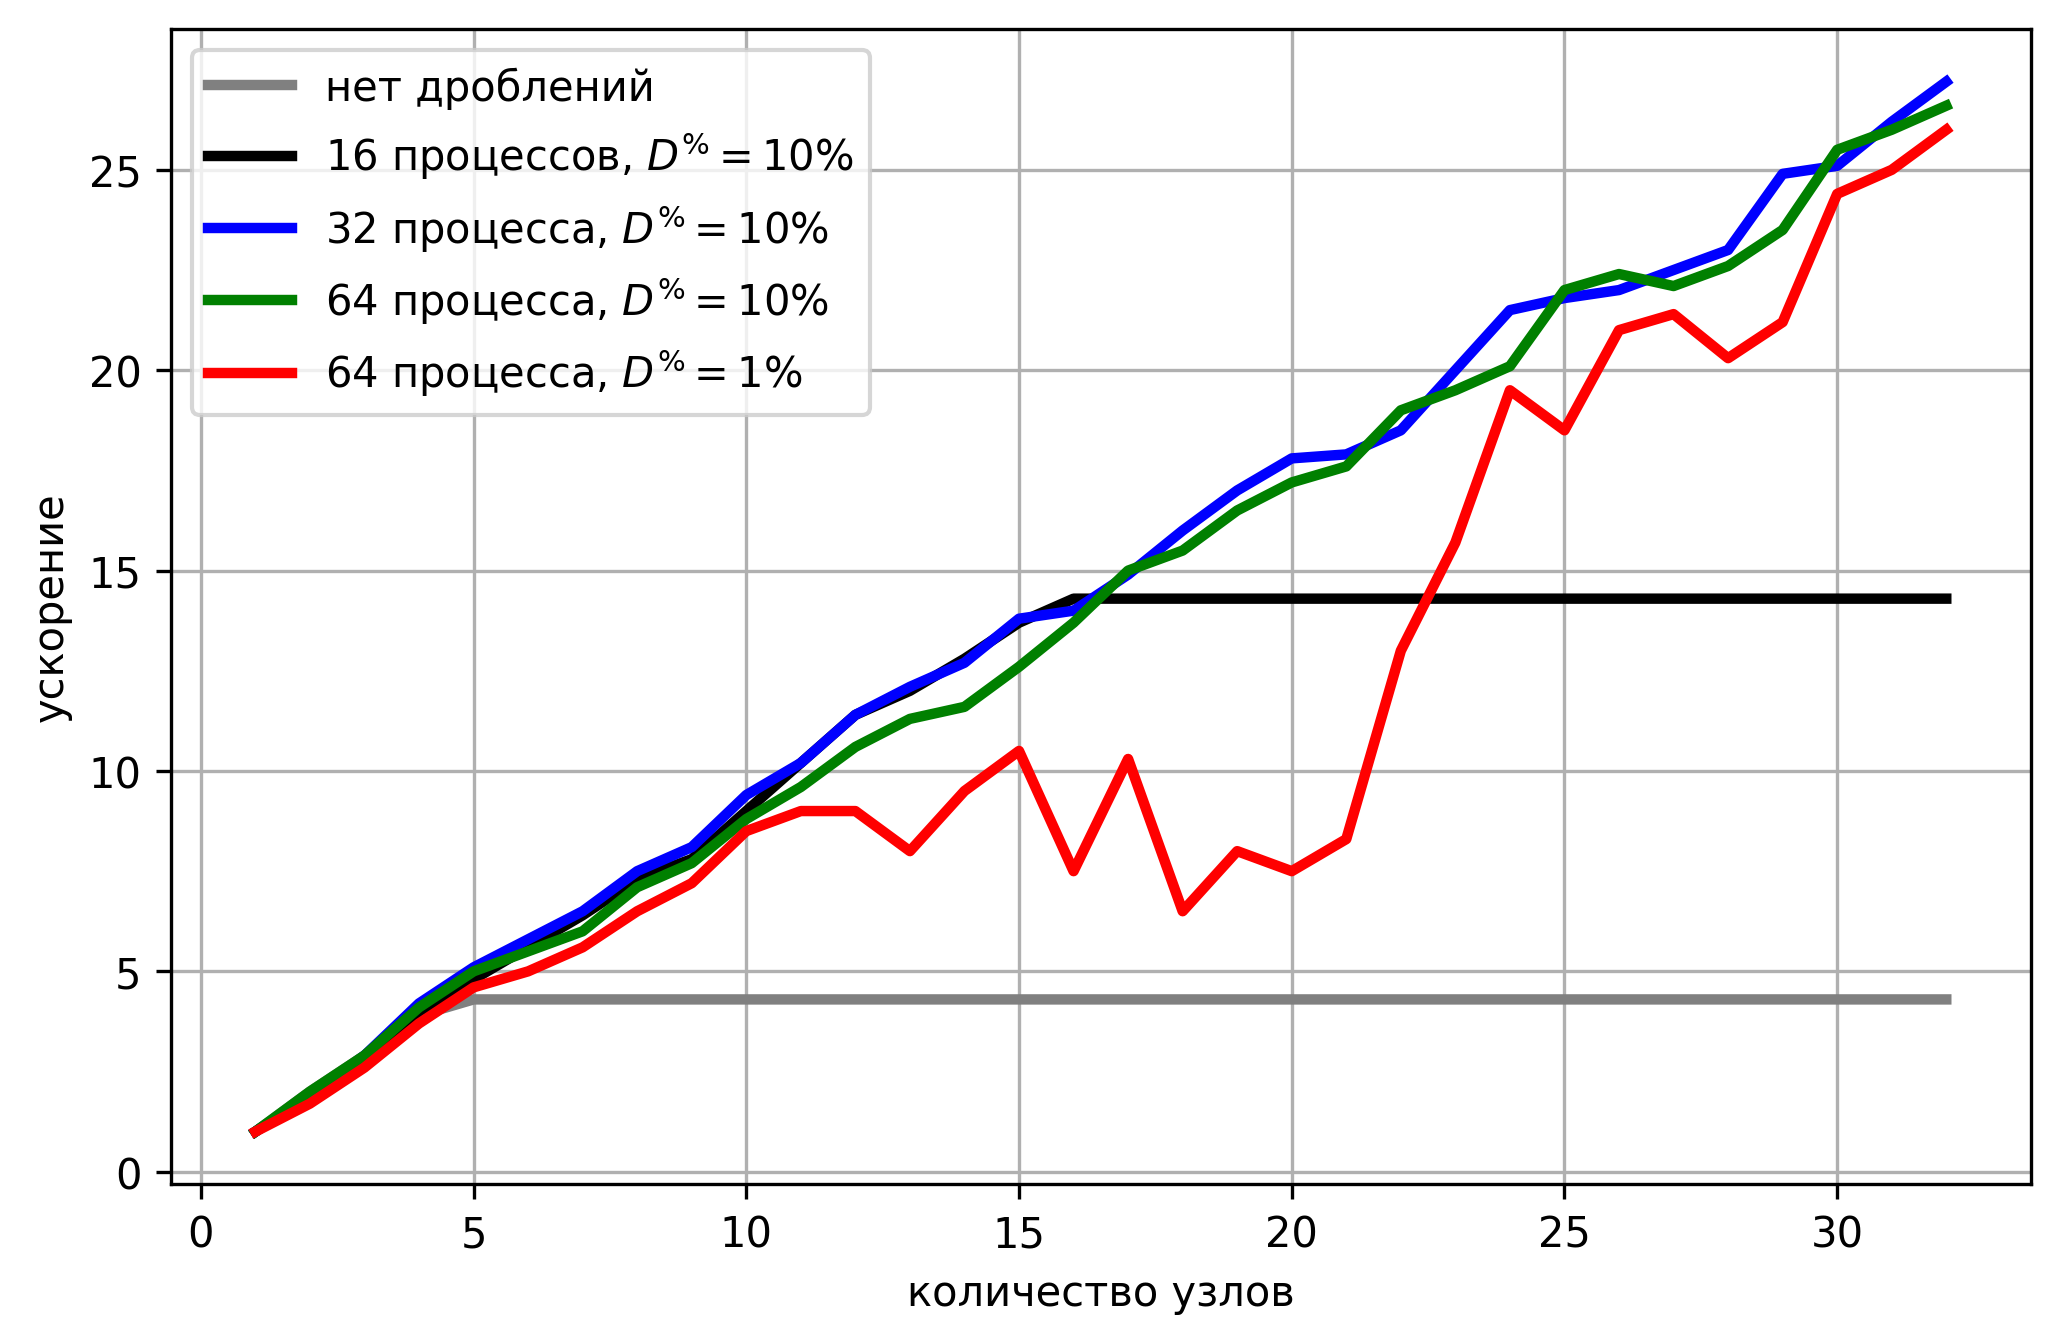
\includegraphics[width=1.0\textwidth]{./pics/text_2_withcut/scaling3.png}
\singlespacing
\caption{Масштабирование вычислений при различных параметрах дробления сетки на 1-32 микропроцессорах Intel Xeon Phi Knights Landing 7290.}
\label{fig:text_2_withcut_scaling3}
\end{figure}

На рис.~\ref{fig:text_2_withcut_scaling3} представлены результаты численных экспериментов на сегменте суперкомпьютера, состоящем из узлов, каждый из которых содержит по одному микропроцессору Intel Xeon Phi Knights Landing 7290.
При проведении расчетов на каждом узле запускался один MPI процесс.
Количество узлов менялось от 1 до 32.
Проанализируем графики ускорения вычислений, представленные на рис.~\ref{fig:text_2_withcut_scaling3}.

Для вычислений на неподготовленной сетке (соответствует графику "нет дроблений") наблюдается ускорение для количества процессов до 5.
Далее ускорение остается на одной и той же отметке (около 4,3) и не меняется при дальнейшем увеличении количества узлов.
Это связано с наличием крупного блока, который мешает равномерному распределению вычислительной нагрузки.

При подготовке сетки для выполнения на 16 процессах (черный график) ускорение также останавливается, но на более высокой отметке (в районе 14,0).
Это также связано с наличием крупного блока, но его размер меньше, чем в случае отказа от дроблений (наиболее крупный блок был раздроблен, что привело к эффективному распределению вычислительной нагрузки для 16 процессов, однако для большего количества процессов размер этого блока препятствует равномерному распределению блоков по процессам).

При подготовке сетки для выполнения на 32 и 64 процессах с допустимым отклонением $D^{\%} = 10\%$ (синий и зеленый графики соответственно) получаем примерно одинаковое возрастание ускорения вычислений с ростом количества узлов.
Это говорит о том, что при подготовка сетки для большего количества процессов, чем реально будет использоваться для запусков, избыточно.

При подготовке сетки для выполнения на 64 процессах с допустимым отклонением $D^{\%} = 1\%$ (красный график) наблюдается сильная просадка по ускорению при использовании количества узлов от 10 до 25.
Это связано с сильным возрастанием количества дроблений, что приводит к увеличению доли межпроцессных обменов.

%----------------------------------

В п.~4.3 рассматриваются вопросы декомпозиции поверхностной неструктурированной расчетной сетки и предлагается алгоритм сглаживания границ между доменами.
Отмечены два метода декомпозиции, различающиеся по показателям эффективности $D$ и $L$.
Метод декомпозиции с помощью \textit{наращивания доменов} порождает неравномерное распределение ячеек по доменам с достаточно гладкими границами.
Метод \textit{иерархического деления пополам} по наиболее протяженному геометрическому направлению наоборот порождает равномерное распределение ячеек по доменам с протяженными <<пилообразными>> границами.

При использовании декомпозиции расчетной сетки основным показателем качества декомпозиции является параметр $D$, так как он отражает равномерность распределения ячеек по разным вычислительным процессам.
Однако если игнорировать остальные показатели, то в процессе декомпозиции могут появляться протяженные <<пилообразные>> границы между доменами, которые приводят к возрастанию параметров качества декомпозиции $L$ и $I$, что негативно сказывается на производительности.
Пример возникновения таких пилообразных границ можно увидеть на рис.~\ref{fig:text_2_smooth_bad_border}.

\begin{figure}[ht]
\centering
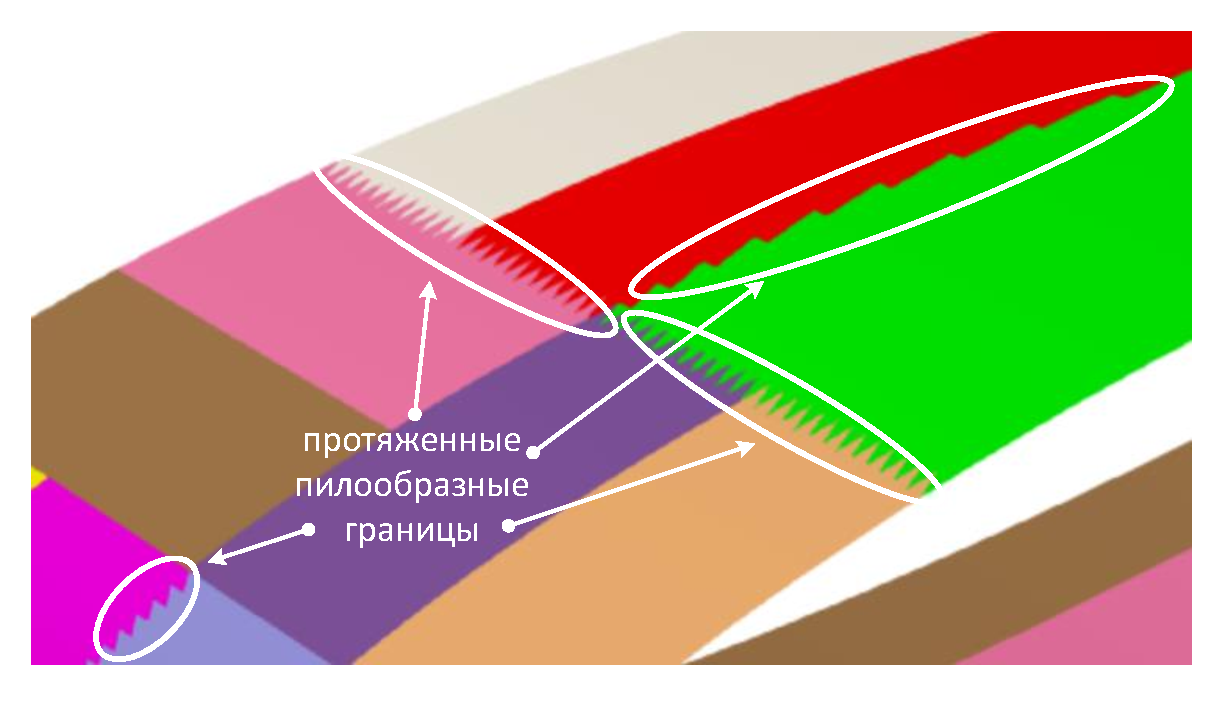
\includegraphics[width=0.6\textwidth]{./pics/text_2_smooth/bad-border.pdf}
\singlespacing
\caption{Возникновение протяженных <<пилообразных>> границ между доменами.}
\label{fig:text_2_smooth_bad_border}
\end{figure}

Алгоритм сглаживания границ между доменами применяется последовательно к каждой паре доменов и направлен на уменьшение длины границы между ними с сохранением баланса количества ячеек в этих доменах.
Граница между двумя доменами может быть представлена в виде набора простых циклов и простых цепей.
При этом простой цикл может быть обработан таким же образом, как и простая цепь, с учетом совпадения первого и последнего узла этой цепи (для такого виртуального размыкания простого цикла может быть выбран произвольный узел этого цикла).
В процессе применения алгоритма сглаживания может быть выполнено виртуальное размыкание всех простых циклов, после чего все образовавшиеся цепи рассматриваются последовательно.
Без ограничения общности можно считать, что мы работаем с одной простой цепью (полученной с помощью записи всех отдельных простых цепей подряд), представляющей границу между парами доменов.

Вначале одним линейным проходом по цепи выполняется поиск всех пригодных для сглаживания границы шаблонов, представленных на рис.~\ref{fig:text_2_smooth_smooth_border}.

\begin{figure}[ht]
\centering
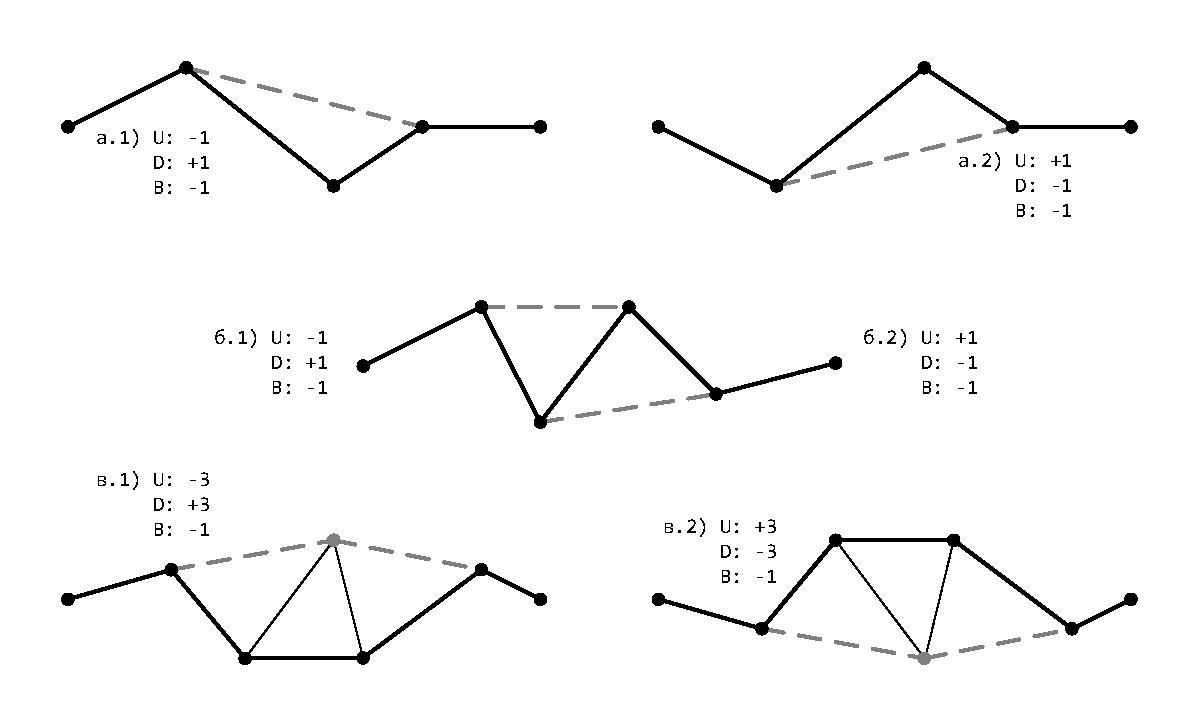
\includegraphics[width=0.8\textwidth]{./pics/text_2_smooth/smooth-border.pdf}
\singlespacing
\caption{Шаблоны элементарных действий сглаживания границ между доменами.}
\label{fig:text_2_smooth_smooth_border}
\end{figure}

После того, как внутри цепи найдены все шаблоны, потенциально пригодные для оптимизации границы, выполняется разметка того, как данные шаблоны могут влиять на другие шаблоны.
С учетом того, что любой шаблон может повлиять только на своих непосредственных соседей, такое действие также выполняется с линейной сложностью относительно длины границы.

Последним шагом применения алгоритма является выбор такого множества шаблонов, которые не влияют друг на друга (то есть могут быть применены все одновременно) и не нарушают суммарного баланса ячеек (так как для нас важнейшим показателем эффективности декомпозиции расчетной сетки является равномерность распределения ячеек по доменам).
После выбора наибольшего возможного набора шаблонов они применяются, и на этом обработка цепи считается завершенной.

Ввиду того, что применение каждого отдельного шаблона уменьшает длину границы на 1, задача поиска оптимального решения может быть сформулирована в виде поиска в множестве шаблонов подмножества максимального размера, не содержащего конфликтующих шаблонов.
Поставленную задачу будем решать методом динамического программирования.
Для этого рассмотрим функцию $B(t, u, x)$, отражающую изменение длины границы при решении задачи на множестве шаблонов $\{ t' \in T : t' \ge t \}$ при условии изменения количества ячеек в домене $U$ на $u$ единиц.
Параметр $x$ является булевым и принимает значение $1$, если шаблон $t$ вошел в решение, и $0$ -- в противном случае.
Решением поставленной задачи является значение $\min(B(t_0, 0, 1), B(t_0, 0, 0))$, где $t_0$ -- первый шаблон на рассматриваемой цепи.

\textbf{Лемма.} \textit{Задача о поиске в множестве шаблонов максимального подмножества без конфликтов может быть решена точно со сложностью алгоритма $O \left( |T| \cdot (U_{max} - U_{min} + 1) \right)$, $U_{min} = \frac{1}{2} \sum_{t \in T}{(U(t) - |U(t)|)}$ -- нижняя граница баланса между доменами, $U_{max} = \frac{1}{2} \sum_{t \in T}{(U(t) + |U(t)|)}$ -- верхняя граница баланса между доменами.}

\begin{figure}[!ht]
\centering
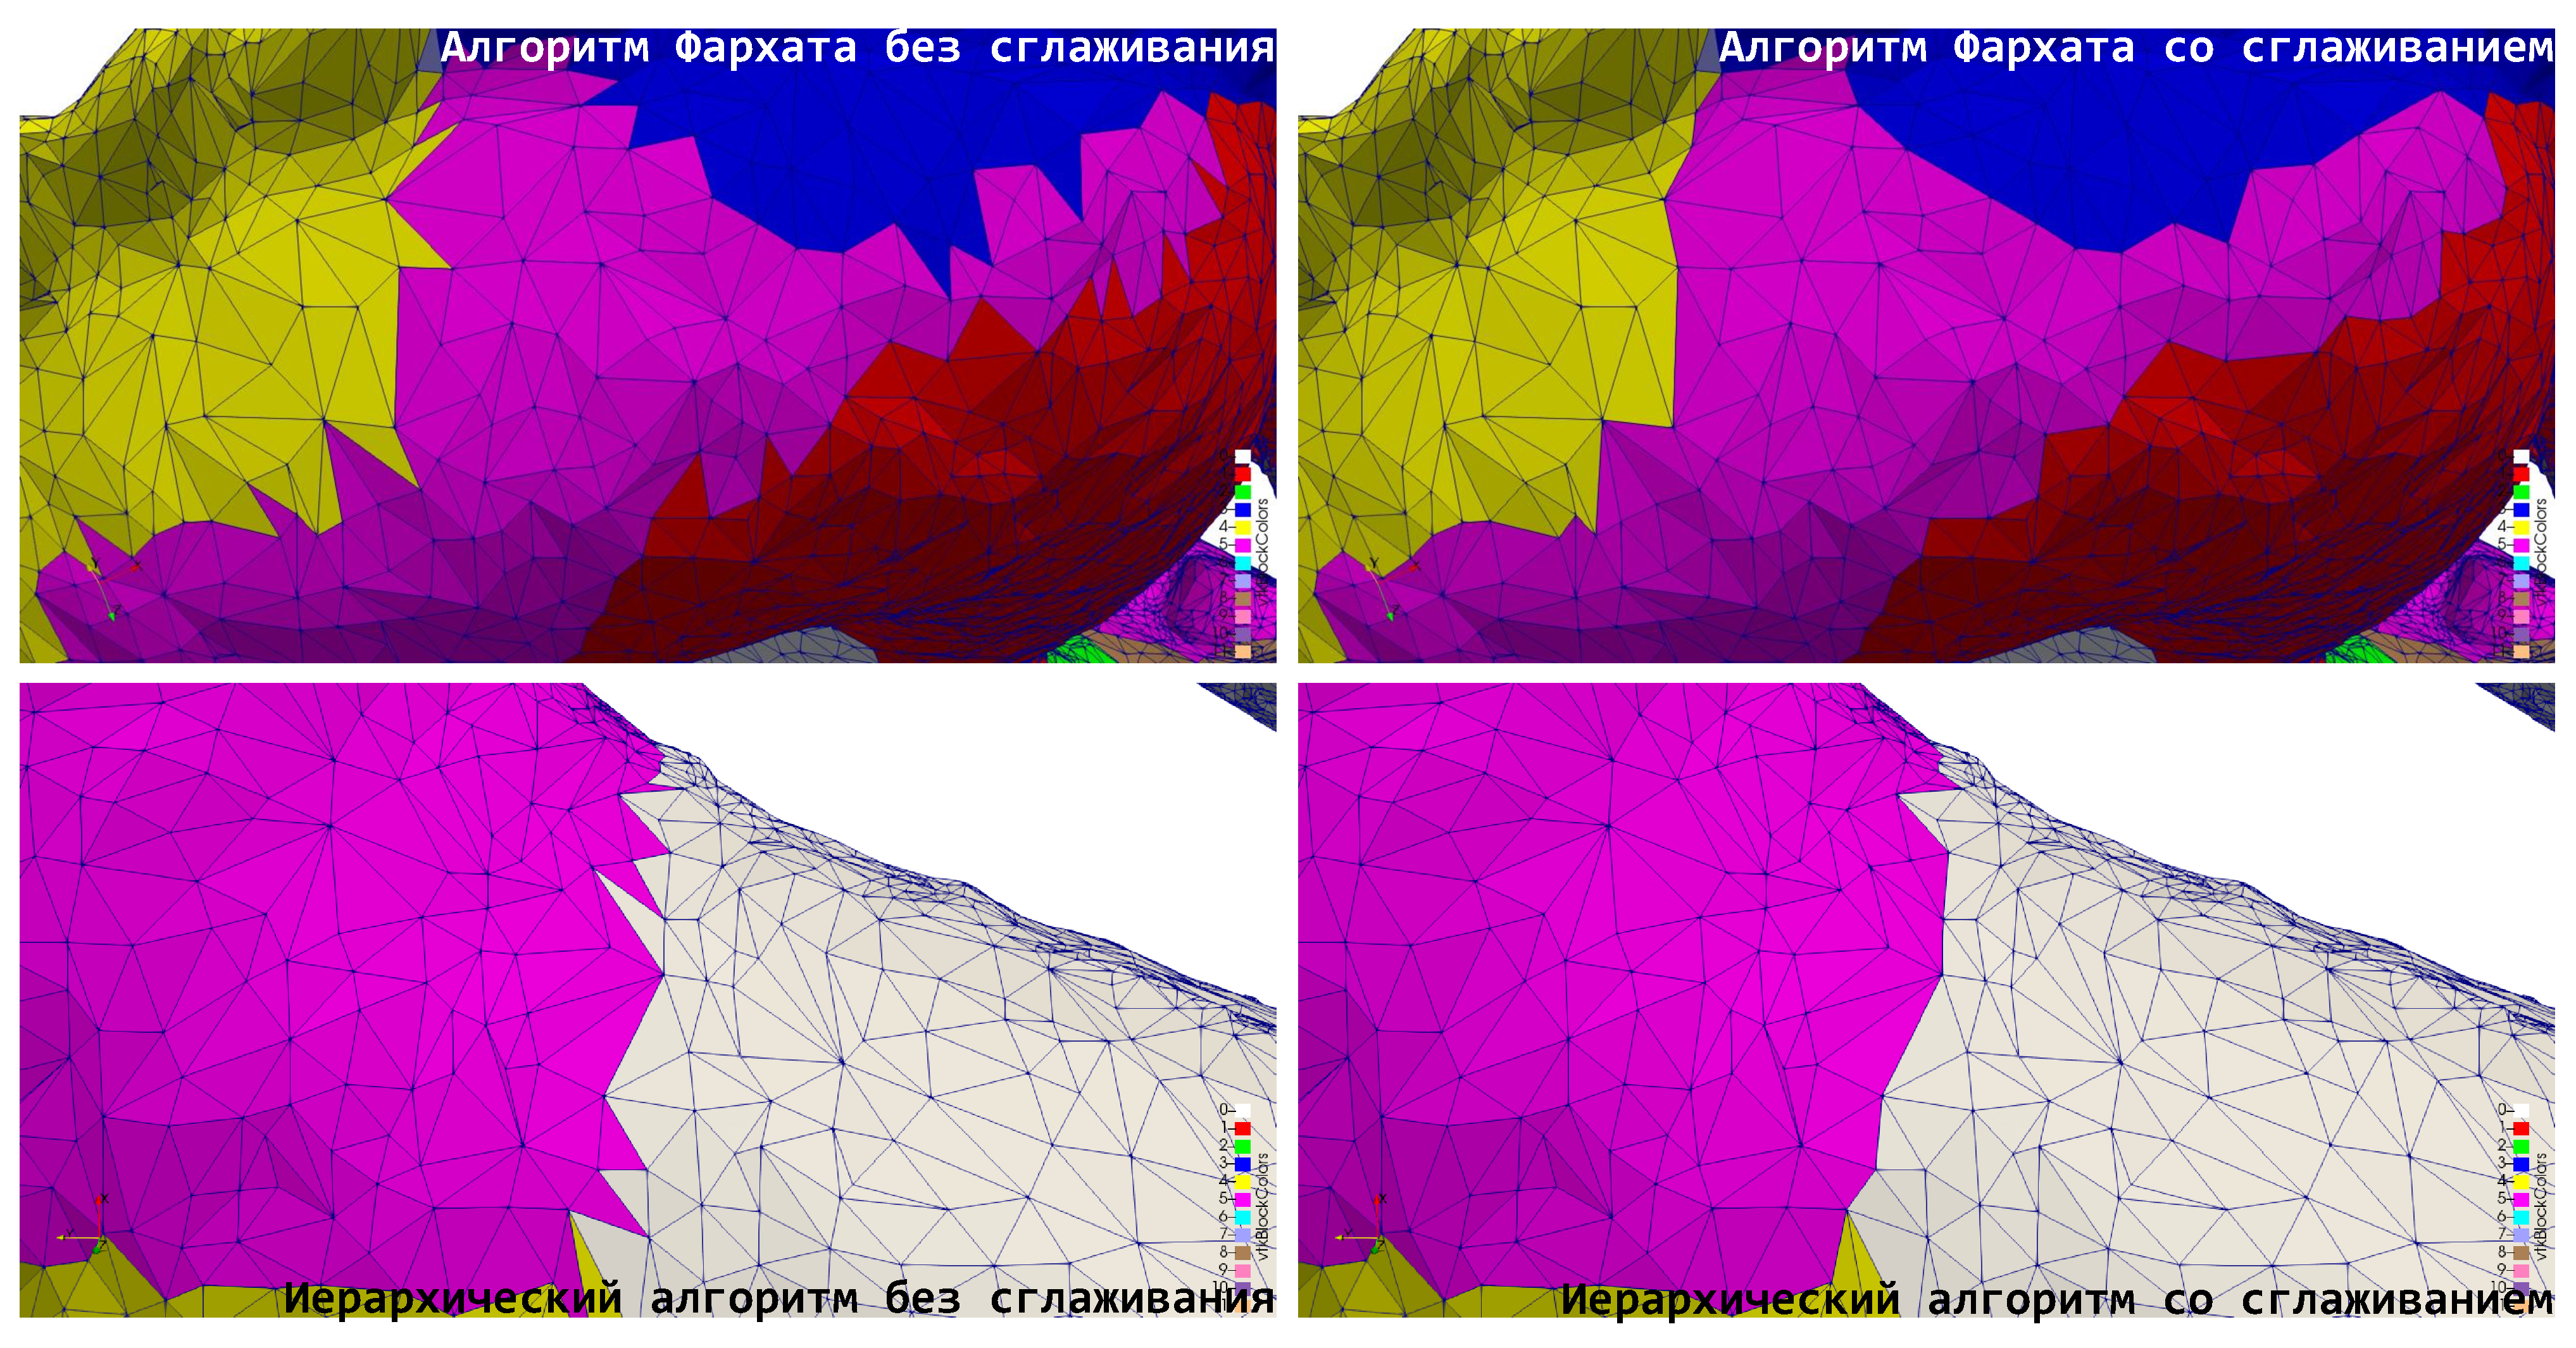
\includegraphics[width=0.8\textwidth]{./pics/text_2_smooth/decomp2.pdf}
\singlespacing
\caption{Визуализация применения сглаживания границ между доменами после работы алгоритма Фархата (сверху) и иерархического алгоритма (снизу).}
\label{fig:text_2_smooth_decomp2}
\end{figure}

На рис.~\ref{fig:text_2_smooth_decomp2} крупным планом продемонстрированы отдельные части тестовой расчетной сетки с отображением ребер ячеек.
На этом рисунке виден эффект от применения алгоритма сглаживания границ между доменами, прежде всего от заключается в устранении одиноких ячеек, которые вторгаются в соседний домен одной своей вершиной.
После применения алгоритма границы между доменами визуально выглядят более гладко, их длина уменьшается.
Применение алгоритма сглаживания границ приводит к сокращению как общего количества граничных ребер, так и длины максимальной границы примерно на 10\%.

\begin{figure}[!ht]
\centering
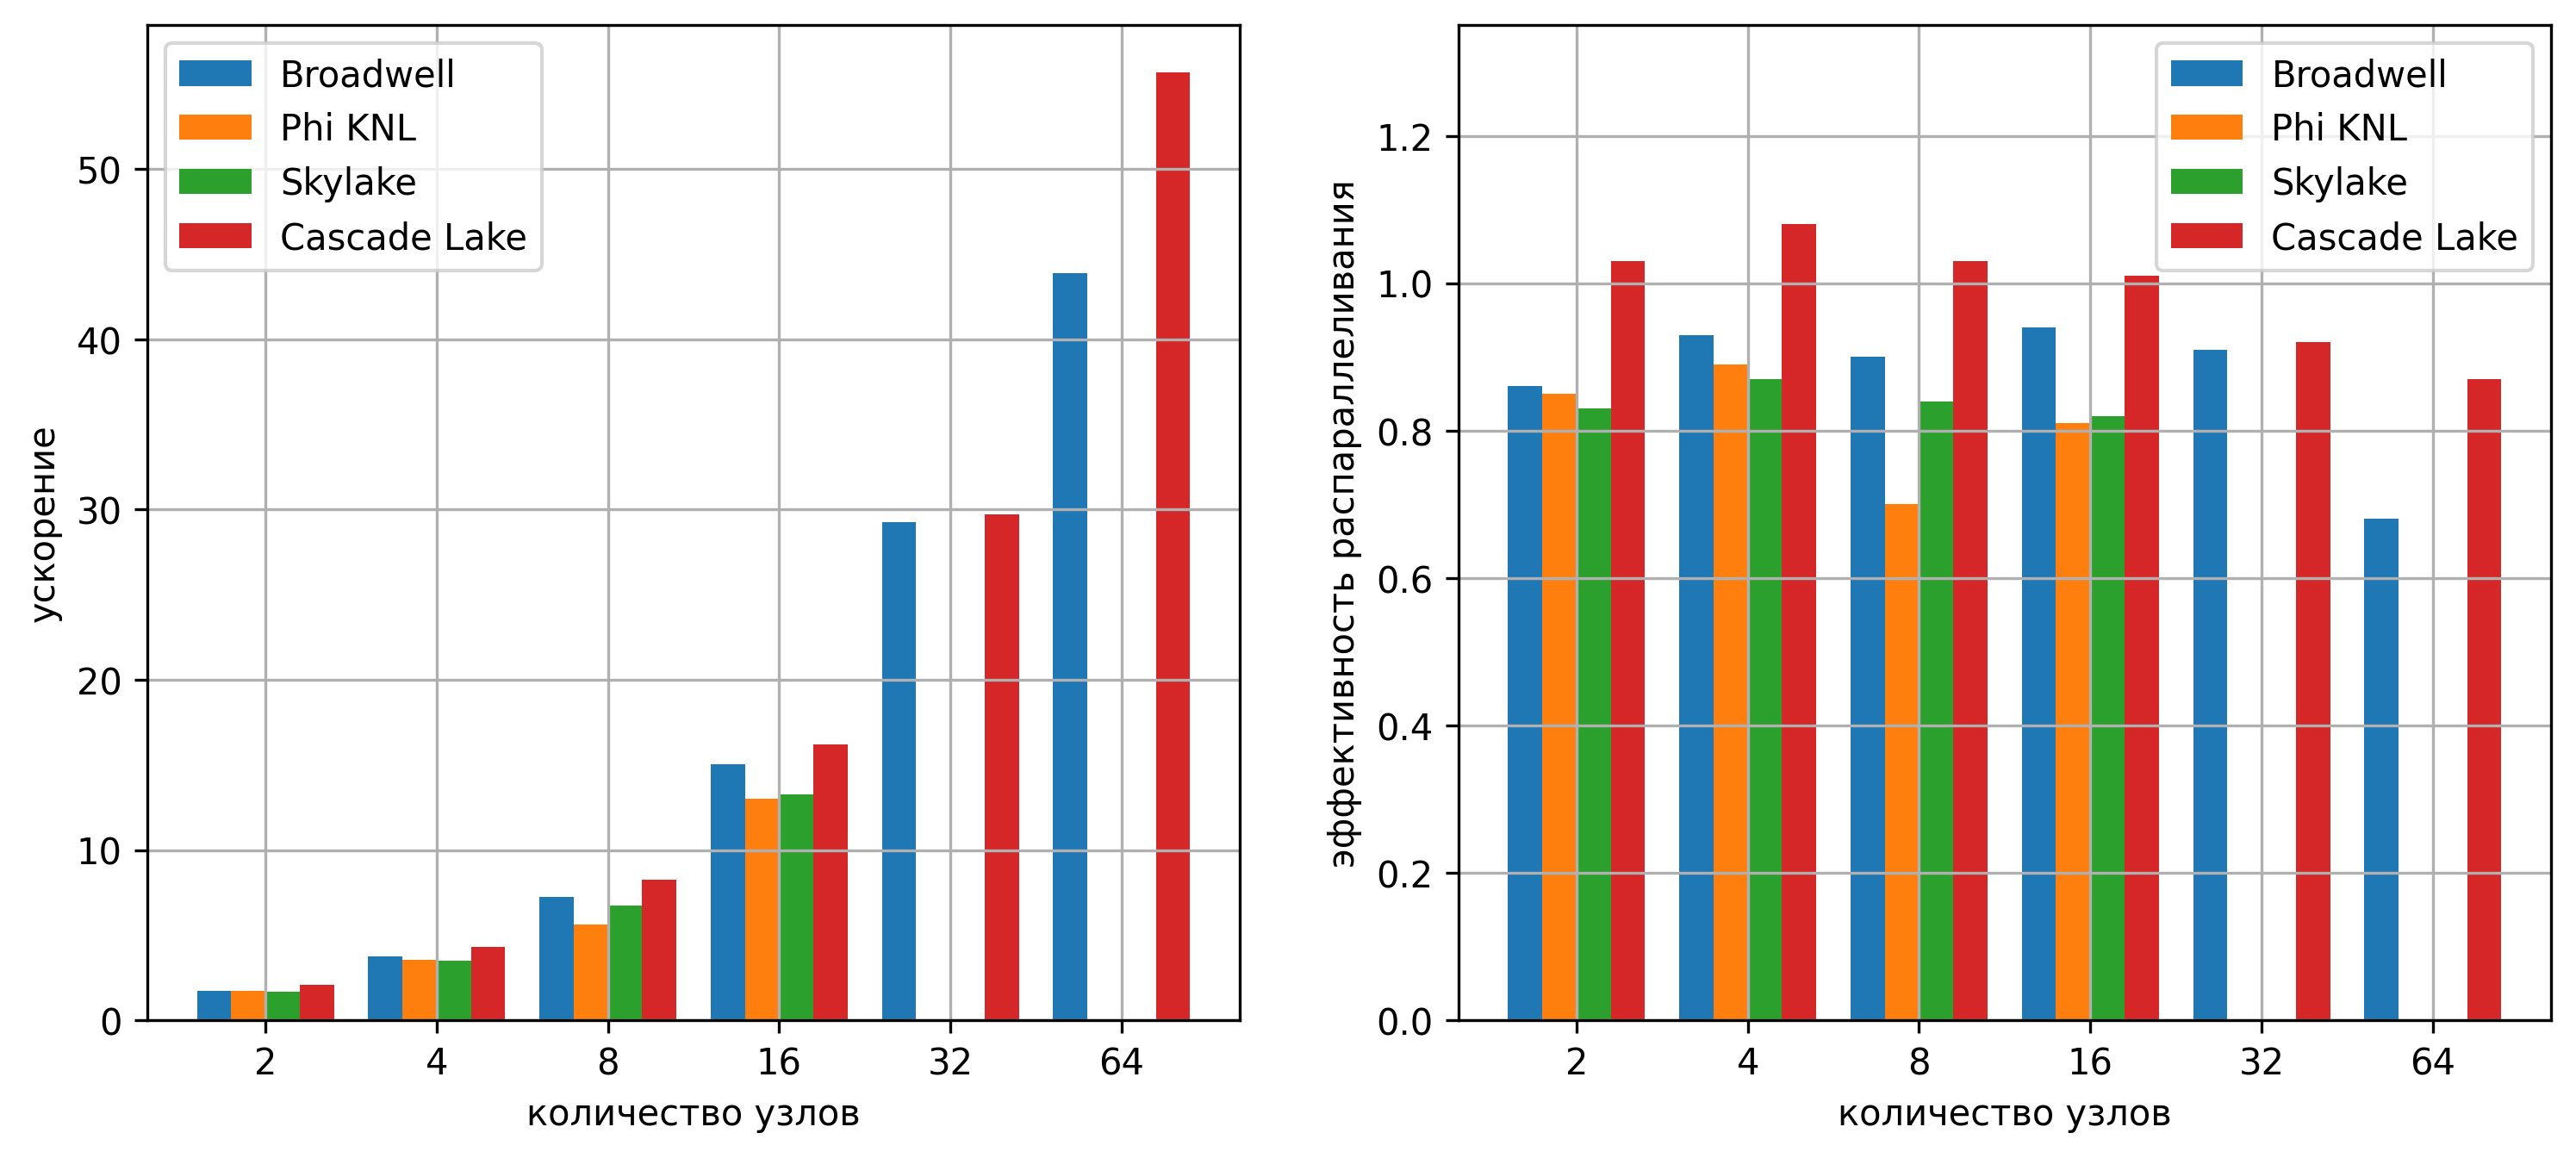
\includegraphics[width=1.0\textwidth]{pics/text_2_scaling/2in1.png}
\singlespacing
\caption{Ускорение (слева) и эффективность распараллеливания (справа) вычислений на сегментах суперкомпьютера МВС-10П при увеличении количества узлов.}
\label{fig:text_2_scaling_speedup_eff}
\end{figure}

Приводится описание эксперимента по замеру ускорения и эффективности распараллеливания задачи расчета ледообразования на поверхностной неструктурированной расчетной сетки с использованием иерархической геометрической декомпозиции сетки со сглаживанием границ между доменами. Замеры производились на вычислительных сегментах суперкомпьютера МВС-10П на базе микропроцессоров Intel разных поколений.
Результаты эксперимента показали, что достигается высокая эффективность распараллеливания вычислений на всех сегментах при использовании до 64 вычислительных узлов (рис.~\ref{fig:text_2_scaling_speedup_eff}).

%----------------------------------

В п.~4.4 Рассматриваются вопросы распараллеливания вычислений на поверхностной неструктурированной сетке на общей памяти.

Рассматривается задача устранения конфликтов по данным при распараллеливании конечно-объемных численных методов на поверхностной неструктурированной расчетной сетке.
Конфликты по данным возникают при параллельной обработке перетекания потоков между ячейками расчетной сетки.
Рассматривается два подхода к устранению конфликтов.

В качестве первого подхода рассматривается использование директивы \texttt{\#pragma omp atomic} при доступе к элементам данных, по которым возможно возникновение конфликтов.
Использование \texttt{\#pragma omp atomic} гарантирует, что указанная команда одновременно будет обрабатываться только одним потоком (то есть, что между чтением старого значения переменной и записью нового значения не попадут операции другого потока).
При большом количестве используемых потоков это может приводить к потерям производительности.

В качестве второго подхода при устранении конфликтов при пересчете потоков через ребра расчетной сетки рассматривается реберная раскраски дуального графа расчетной сетки.
При разбиении ребер дуального графа на множества без конфликтов, каждое из этих множество может быть обработано независимо в параллельном режиме.

Доказывается возможность реберной раскраски дуального графа поверхностной неструктурированной расчетной сетки в 5 и 4 цвета с линейной сложностью по количеству ребер, а также приводится квадратичный алгоритм раскраски в 3 цвета, основанный на базе работ [Курапов, Давидовский, Толок].

Проведены эксперименты по сравнению двух рассмотренных методов устранения конфликтов (рис.~\ref{fig:text_3_edge_coloring_11}).

\begin{figure}[ht]
\centering
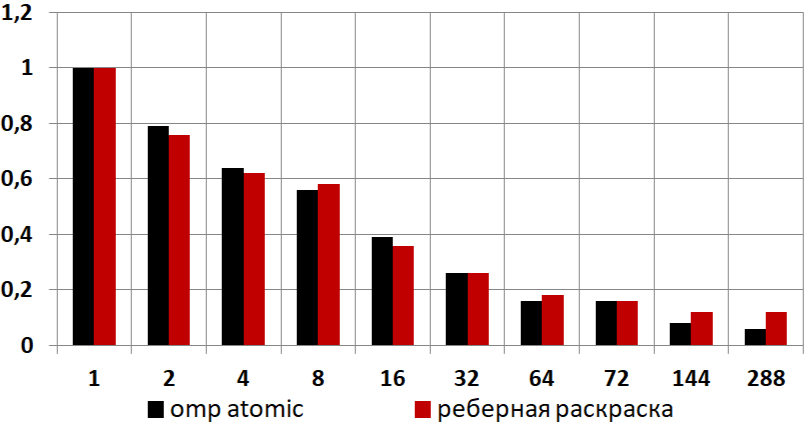
\includegraphics[width=1.0\textwidth]{./pics/text_3_edge_coloring/11-chart.png}
\singlespacing
\caption{Эффективность распараллеливания пересчета потоков для разных способов устранения конфликтов по данным.}
\label{fig:text_3_edge_coloring_11}
\end{figure}

Эксперименты показали, что метод устранения конфликтов с помощью реберной раскраски дуального графа приводит к существенному ускорению расчетов на большом количестве используемых потоков.
Расчеты проводились на микропроцессоре Intel Xeon Phi KNL, поддерживающем до 288 потоков.

Рассматривается сравнение эффективности распараллеливания вычислений на общей памяти для вычислительных узлов на базы микропроцессоров Intel.
Расчеты проводились для вычислительных узлов на базе микропроцессоров Haswell, Broadwell, Phi KNL, Skylake и Cascade Lake.
Сравнение выполнялось на примере газодинамического решателя, использующего метод Годунова на базе точного решения задаче о распаде разрыва.

\begin{figure}[ht]
\centering
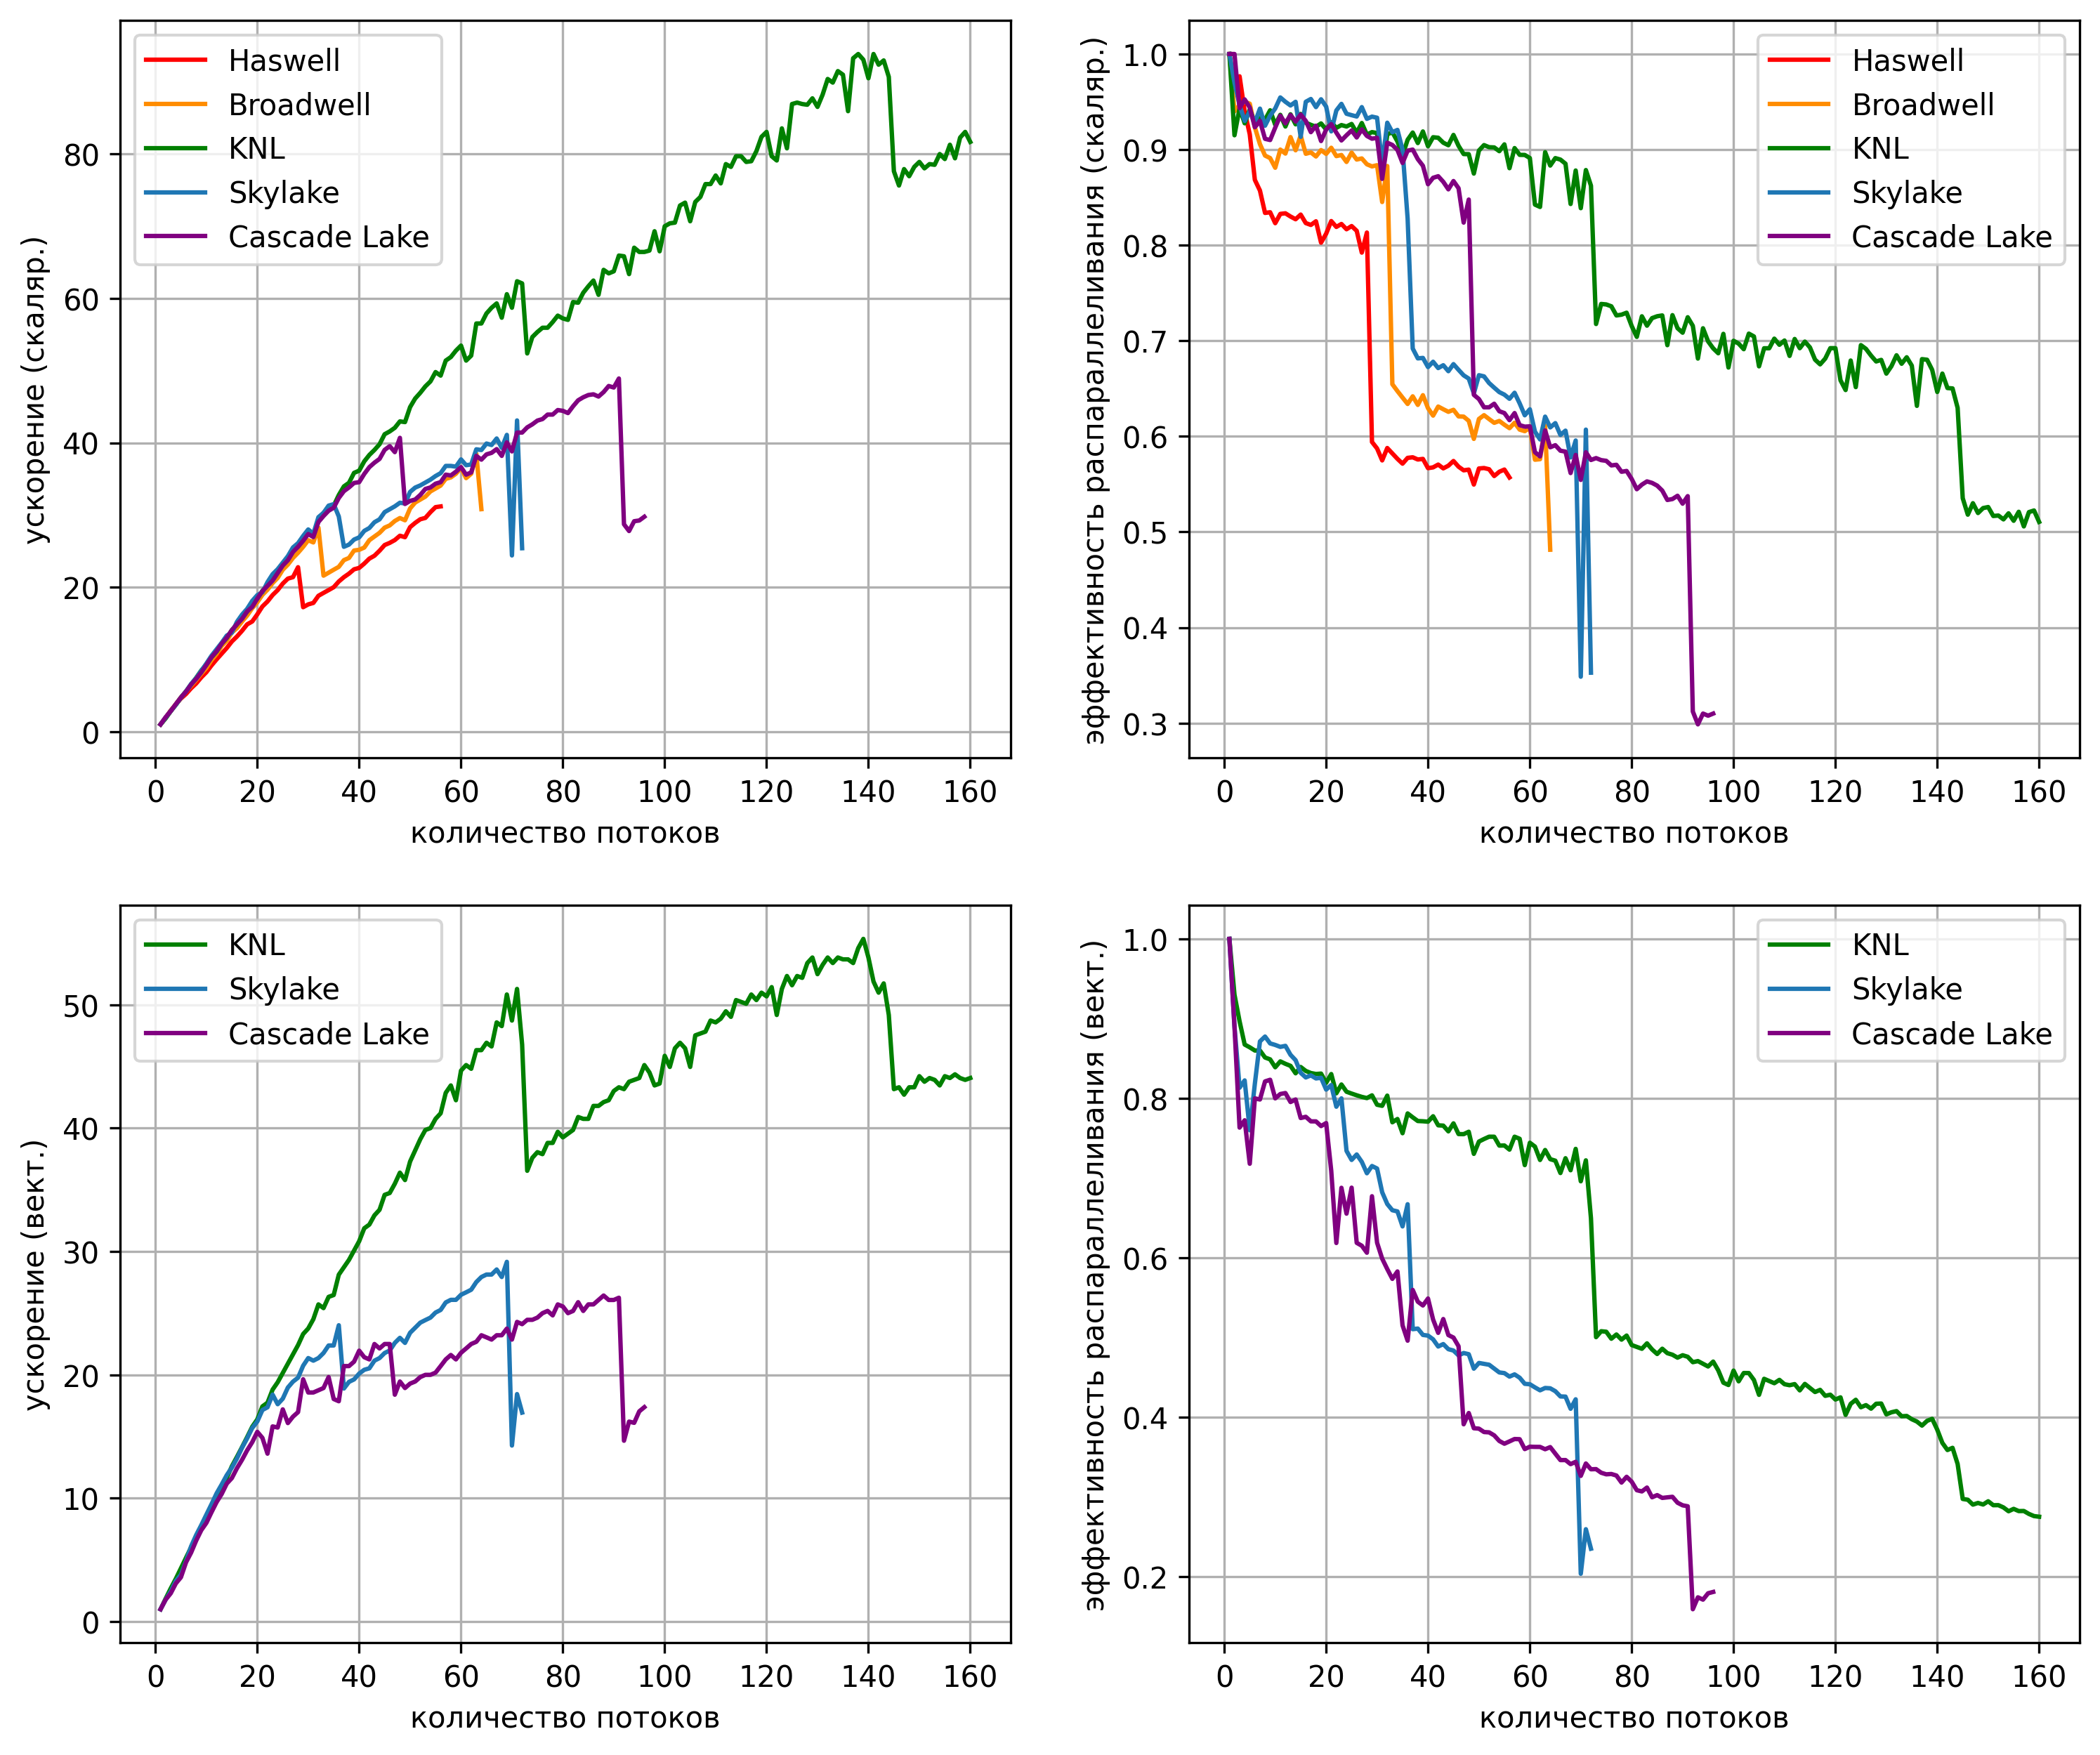
\includegraphics[width=1.0\textwidth]{./pics/text_3_omp2/main_chart.png}
\singlespacing
\caption{Графики ускорения и эффективности распараллеливания скалярной и векторизованной версии римановского решателя для микропроцессоров Haswell, Broadwell, KNL, Skylake и Cascade Lake.}
\label{fig:text_3_omp2}
\end{figure}

На рис.~\ref{fig:text_3_omp2} сверху слева представлены графики ускорения скалярной версии римановского решателя при увеличении количества потоков с 1 до 160.
Для каждого вычислительного узла явно просматриваются отрезки квазилинейного ускорения, которые завершаются заметными провалами.
Длина этих отрезков во всех случаях равняется суммарному количеству ядер в узле, а провалы обусловлены конфликтами за аппаратные ресурсы.
При этом стоит отметить, что хоть максимальное количество доступных потоков для вычислительного узла на базе микропроцессора KNL равняется 288, однако на графике не показаны значения больше 160, так как сверх этого значения наблюдается только деградация производительности, и наиболее эффективное использование зафиксировано в диапазоне потоков 140-144.
Также можно отметить, что для всех микропроцессоров ускорение близко к линейному до тех пор, пока каждый поток запущен на своем отдельном ядре.

На рис.~\ref{fig:text_3_omp2} снизу слева представлены аналогичные данные, но уже для векторизованной версии римановского решателя (соответственно только для микропроцессоров KNL, Skylake, Cascade Lake).
Из графиков видно, что характер ускорения для KNL практически не поменялся, тогда как Skylake и Cascade Lake демонстрируют серьезную деградацию ускорения вычислений уже на небольшом количестве потоков.

На рис.~\ref{fig:text_3_omp2} справа приведены данные показателей эффективности масштабирования римановского решателя (скалярной и векторизованной версии).
Данные иллюстрации более информативные.
Например, из рис.~\ref{fig:text_3_omp2} сверху справа видно, что масштабируемость при количестве потоков, не превышающем количество ядер вычислительного узла, находится для всех микропроцессоров на хорошем уровне в диапазоне 0,8 - 1,0.
Рис.~\ref{fig:text_3_omp2} снизу справа наглядно демонстрирует хорошую масштабируемость векторизованного римановского решателя для микропроцессора KNL с показателем, близким к 0,8 вплоть до использования 72 потоков, тогда как узлы на базе микропроцессоров Skylake и Cascade Lake деградируют на масштабировании векторизованной версии римановского решателя на достаточно небольшом количестве потоков.

%---------------------------------------------------------------------------------------------------

\textbf{Пятая глава} посвящена проблемам \textit{векторизации программного кода}.
Векторизация является низкоуровневой оптимизацией распараллеливания вычислений на уровне отдельных инструкций, векторные инструкции поддержаны во всех современных микропроцессорных архитектурах (x86, ARM, Power, <<Эльбрус>>, LoongArch, Sunway и других), правильное применение векторизации способно кратно увеличить производительность приложений.
Уникальный набор векторных инструкций AVX-512 поддерживает возможность выборочной обработки элементов векторов с помощью \textit{векторных масок}, что делает возможным векторизацию сложного программного контекста с обилием операций передачи управления, гнездами циклов и вызовами функций.
Существует проблема недостаточно эффективного применения векторизации оптимизирующим компилятором для сложного программного контекста.
Для оценки эффективности применения векторизации используются понятия \textit{ширина векторизации} $w = \frac{v}{t}$ (где $v$ -- размер векторного регистра, $t$ -- размер типа расчетных данных), \textit{ускорение от применения векторизации} $s_{vec} = \frac{T}{T_v}$ (где $T$ -- время выполнения невекторизованной версии кода, $T_v$ -- время выполнения векторизованной версии кода), \textit{эффективность векторизации} $e_{vec} = \frac{s_{vec}}{w}$.

%----------------------------------

В п.~4.1 приведено описание набора векторных инструкций AVX-512, перечислены основные подмножества операций и рассмотрены особенности этого набора.
В качестве основной отличительной черты этого набора инструкций, позволяющей векторизовать программный контекст со сложным управлением, названа возможность выполнения векторных инструкций с использованием векторных масок, определяющих индексы элементов, для которых в выходной регистр записывается результат операции.

%----------------------------------

В п.~4.2 рассматривается векторизация программного кода путем выделения однотипных операций и объединения их в векторные аналоги на примере операций с матрицами малой размерности.
На примере матричных операций показано, что от способа выделения однотипных операций для объединения в векторные аналоги существенным образом зависит производительность результирующего кода.
Также продемонстрировано, что низкая \textit{плотность векторных масок} (количество единичных битов в маске) в результирующем коде негативно сказывается на производительность.

%----------------------------------

В п.~4.3 вводится понятие \textit{плоского цикла} как удобного контекста для векторизации вычислений, что делает его предпочтительной формой компоновки программного кода для успешного автоматического применения векторизации оптимизирующим компилятором.

\begin{figure}[ht]
\centering
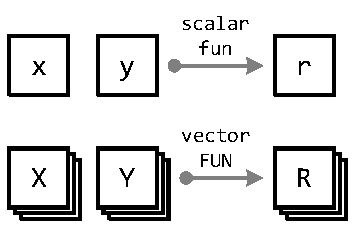
\includegraphics[width=0.3\textwidth]{./pics/text_4_flat/fun.pdf}
\singlespacing
\caption{Схема выполнения скалярного блока block и аналогичного векторного блока BLOCK.}
\label{fig:text_4_vec_flat_fun_FUN}
\end{figure}

Основная идея плоского цикла состоит в объединении нескольких экземпляров \textit{скалярного блока} (в количестве, равном ширине векторизации $w$) в единый \textit{векторный блок} (рис.~\ref{fig:text_4_vec_flat_fun_FUN}), состоящий из аналогичных векторных операций.
Здесь $w$ экземпляров скалярного блока $block(x, y) \rightarrow r$ со скалярными входными данными $x$, $y$ и скалярным результатом $r$ объединены в векторный блок $BLOCK(X, Y) \rightarrow R$ с векторными входными данными $X$, $Y$ и векторным результатом $R$.

\begin{table}[!ht]
\centering
\singlespacing
\caption{Инструкции AVX-512 для работы с вещественными числами \\ и их семантика.}
\bigskip
\label{tbl:text_4_flat_avx512semantic}
\begin{tabular}{ | c | c | }
  \hline
  Имя инструкции & Семантика инструкции \\ \hline\hline
  \makecell{VMOVAPS, VMOVUPS, VSQRTPS, \\ VGETEXPPS, VGETMANTPS, \\ VRCP14PS, VREDUCEPS, VRNDSCALEPS, \\ VRSQRT14PS, VSCALEFPS} & $\begin{matrix} R = op \ A \\ R = \check{P} \ ? \ (op \ A) : R \\ R = \check{P} \ ? \ (op \ A) : 0 \end{matrix}$ \\ \hline
  \makecell{VADDPS, VANDPS, VANDNPS, VDIVPS, \\ VMAXPS, VMINPS, VMULPS, VORPS, \\ VSUBPS, VRANGEPS} & $\begin{matrix} R = op \ A, B \\ R = \check{P} \ ? \ (op \ A, B) : R \\ R = \check{P} \ ? \ (op \ A, B) : 0 \end{matrix}$ \\ \hline
  \makecell{VFMADD*PS, VFMSUB*PS, \\ VFNMADD*PS, VFNMSUB*PS} & $\begin{matrix} R = op \ R, A, B \\ R = \check{P} \ ? \ (op \ R, A, B) : R \\ R = \check{P} \ ? \ (op \ R, A, B) : 0 \end{matrix}$ \\ \hline
  \makecell{VCMPPS} & $\begin{matrix} \check{P} = op \ A, B \\ \check{P} = \check{Q} \ ? \ (op \ A, B) : 0 \end{matrix}$ \\ \hline
  \makecell{VBLENDPS} & $\begin{matrix} R = \check{P} \ ? \ A : B \end{matrix}$ \\ \hline
\end{tabular}
\end{table}

В качестве плоского цикла рассматривается цикл \texttt{for}, в котором индуктивная переменная $i$ последовательно принимает значения от $0$ до $w - 1$ (\texttt{for (int i = 0; i < w; ++i)}).
К плоскому циклу предъявляются следующие требования.
На $i$-ой итерации все обращения к данным на запись имеют вид \texttt{a[i]}, а обращения к данным на чтение либо имеют вид \texttt{a[i]}, либо являются чтением скаляров.
Все массивы данных, обращение к которым на $i$-ой итерации цикла имеет вид \texttt{a[i]}, выровнены в памяти на размер вектора.
В цикле отсутствуют межитерационные зависимости.

Программный контекст, удовлетворяющий требованиям, предъявляемым к плоским циклам, является удобным для векторизации и зачастую может быть заменем на векторный блок, а логика работы многих векторных инструкций может быть представлена в виде плоского цикла и записана в предикатной форме, как это показано в таблице~\ref{tbl:text_4_flat_avx512semantic}.

Без ограничения общности можно считать, что плоский цикл содержит произвольное количество итераций $n$, так как он с помощью расщепления цикла по индуктивной переменной может быть разбит на $\lfloor \frac{n}{w} \rfloor$ циклов с $w$ итерациями и возможно еще один с $n - \lfloor \frac{n}{w} \rfloor w$ итерациями (\textit{эпилог цикла}).

Обсуждается применение автоматической векторизации к программному коду, представленному в виде композиции плоских циклов, а также демонстрируется негативное влияние, оказываемое отклонениеми от требований плоского цикла (такие циклы называются \textit{квазиплоскими}) на производительность результирующего кода.
В качестве программного контекста рассматривается реализация газодинамического решателя с использованием метода погруженной границы для аппроксимации граничных условий.

\begin{figure}[ht]
\centering
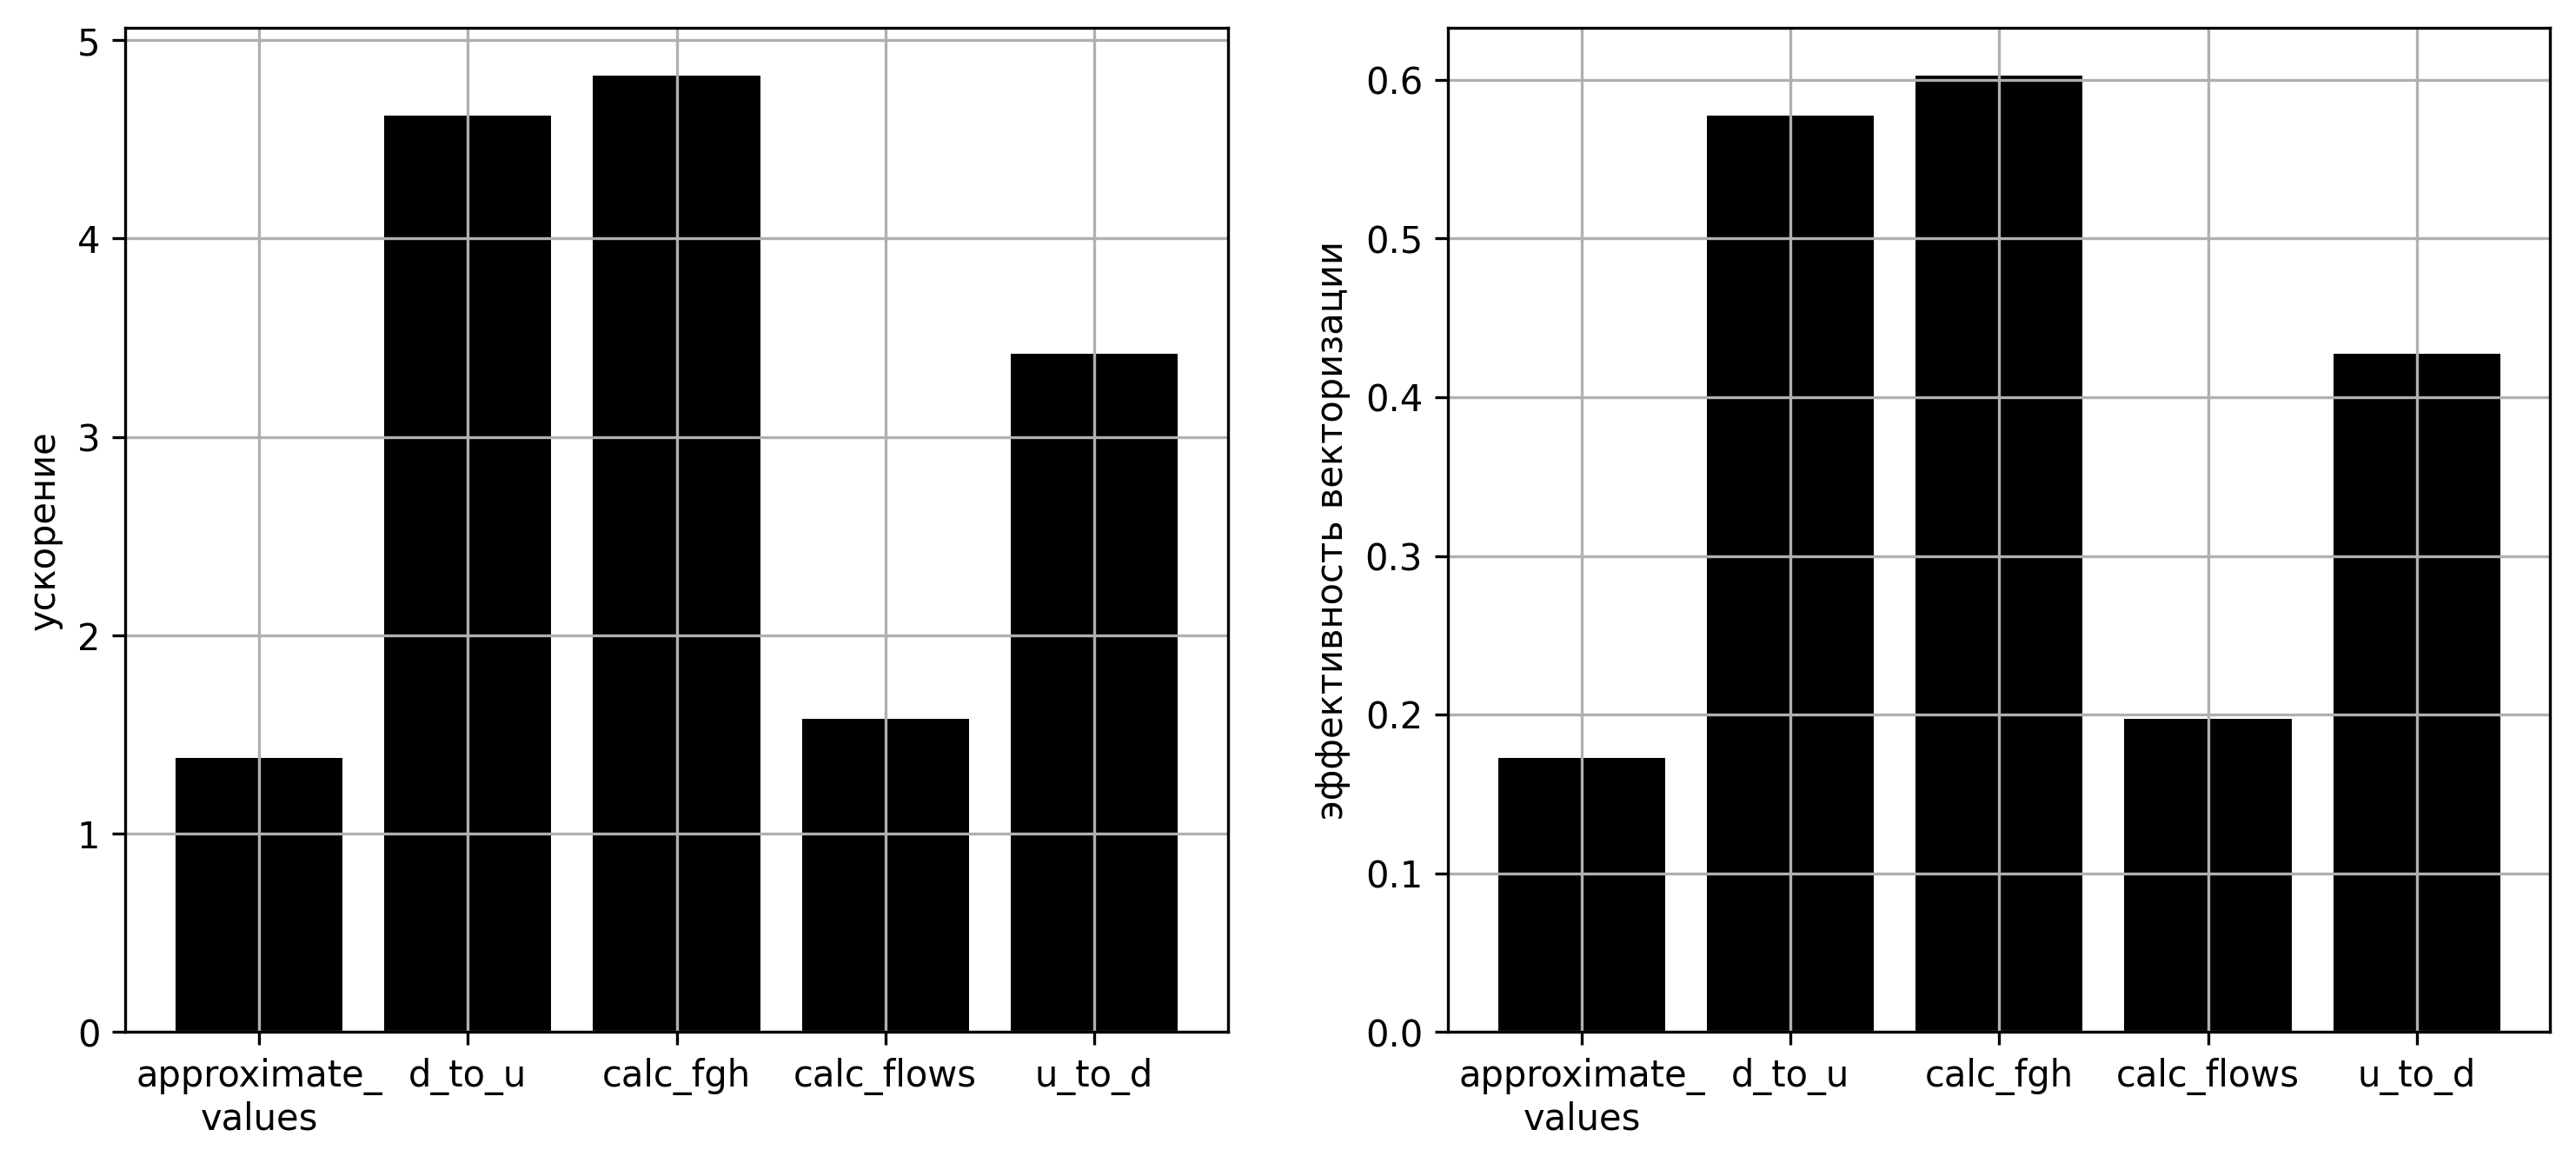
\includegraphics[width=0.5\textwidth]{./pics/text_4_ibm/diagr2.png}
\singlespacing
\caption{Ускорение кода и эффективность векторизации отдельных функций газодинамического решателя.}
\label{fig:text_4_ibm_diagr2}
\end{figure}

Для приведения программного кода к виду плоских циклов применяется организация данных в виде набора массивов, а также расщепление циклов по константному условию для сокращения количества операций передачи управления внутри цикла.

Векторизованные версии функций, полностью удовлетворяющие требованиям плоских циклов, продемонстрировали более высокую эффективность векторизации (зеленые столбцы на рис.~\ref{fig:text_4_ibm_diagr2}).

%----------------------------------

В п.~4.4 рассматривается оптимизация \textit{выноса маловероятного региона из плоского цикла}.
Оптимизация заключается в сохранении условий входа в маловероятный регион во временный массив и удалении этого региона из основного цикла.
Основной цикл, свободный от удаленного региона, может быть успешно векторизован, а вынесенный маловероятный регион может быть обработан в отдельном цикле согласно сохраненным условиям.

%----------------------------------

В п.~4.5 рассматривается процедура \textit{слияния путей исполнения по условию} внутри плоского цикла с помощью постановки операций из параллельных скалярных блоков под сооответствующие предикаты.

\begin{figure}[ht]
\centering
\begin{tabular}{ll}
	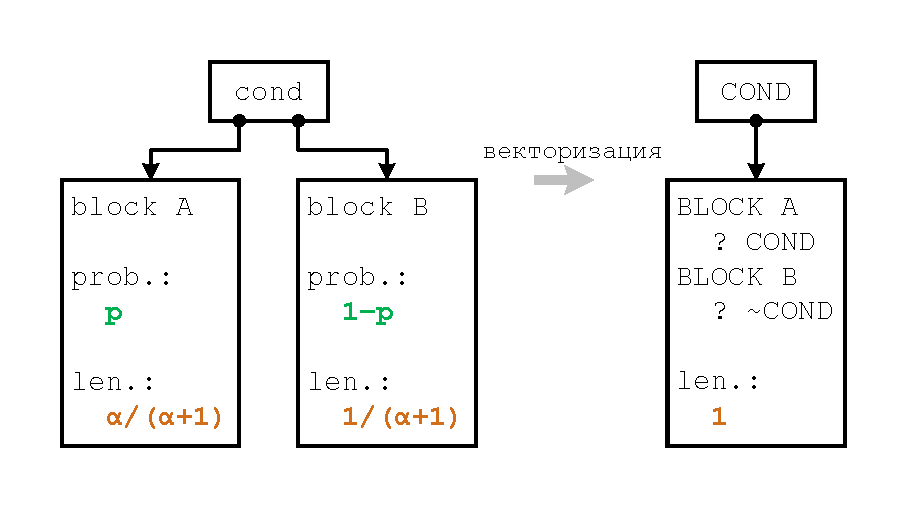
\includegraphics[width=0.45\textwidth]{./pics/text_4_vec_mrg_under_cond/cond.pdf}
	&
	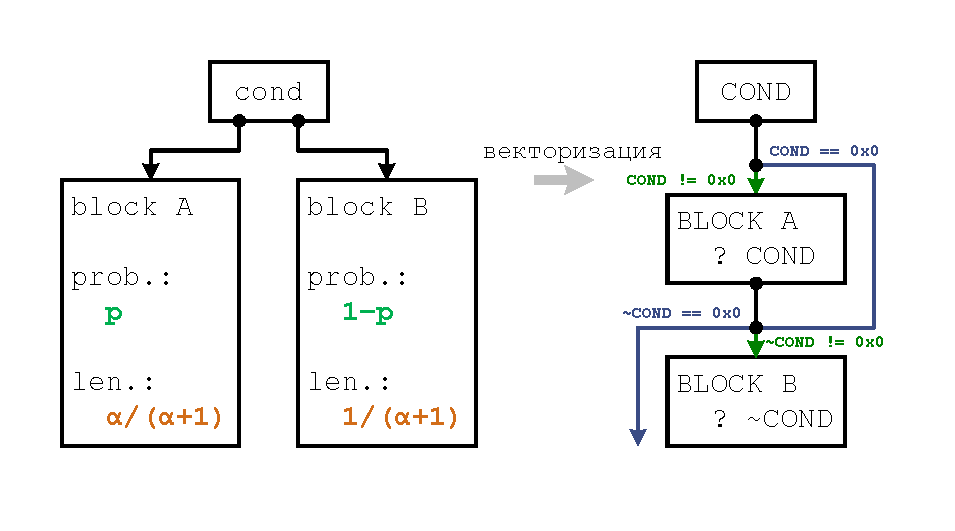
\includegraphics[width=0.45\textwidth]{./pics/text_4_vec_check_mask/cond.pdf}
\end{tabular}
\singlespacing
\caption{Схема векторизации со слиянием двух скалярных блоков по условию без проверки векторной маски (слева) и с проверкой (справа).}
\label{fig:text_4_vec_mrg_under_cond_cond}
\end{figure}

\begin{figure}[ht]
\centering
\begin{tabular}{ll}
	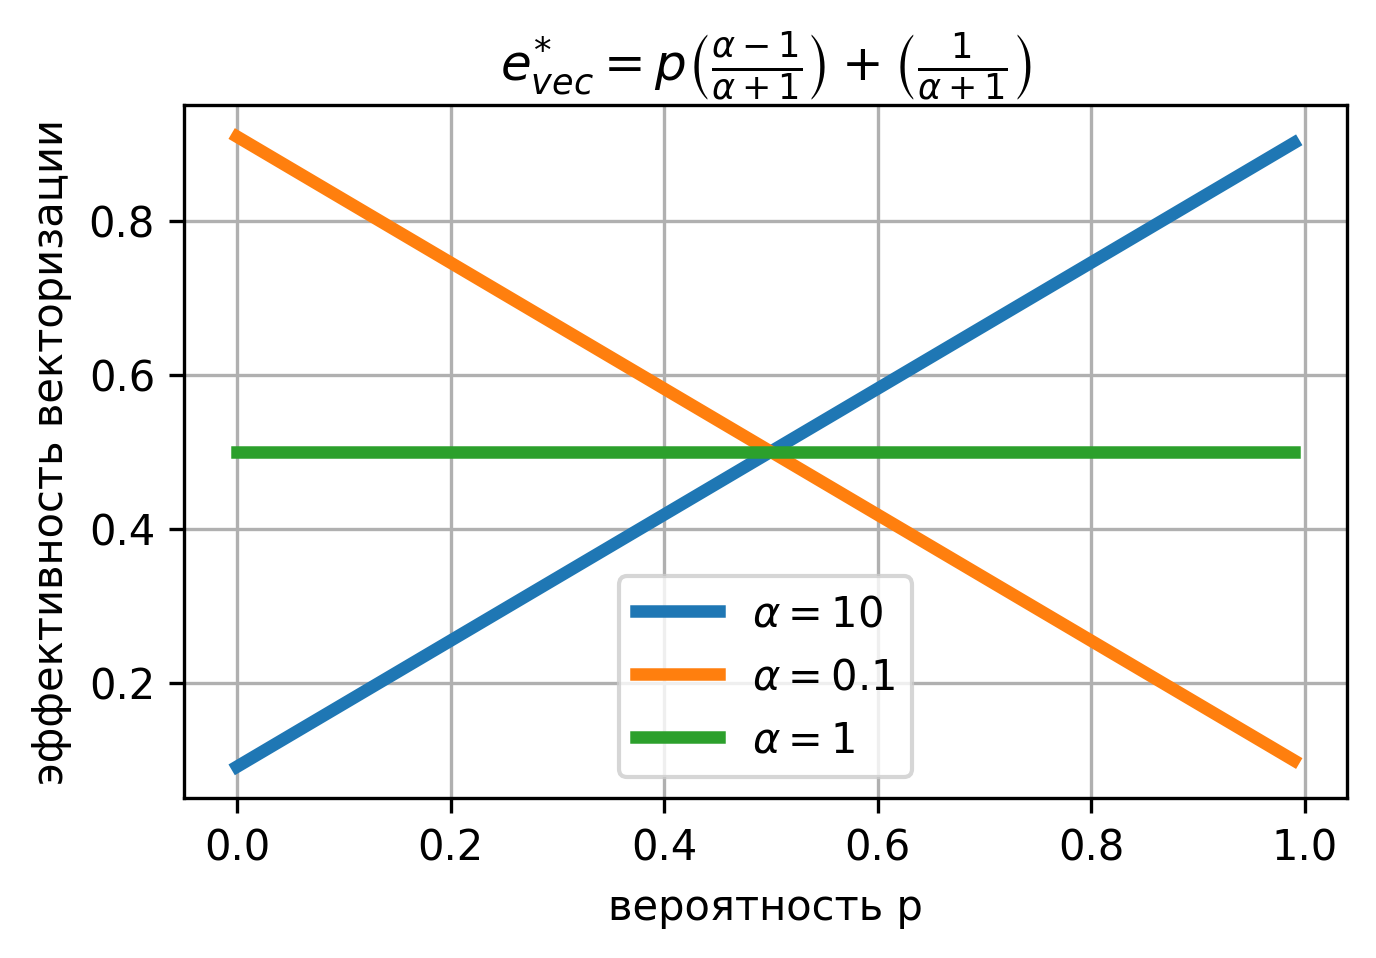
\includegraphics[width=0.45\textwidth]{./pics/text_4_vec_mrg_under_cond/chart_e_merged.png}
	&
	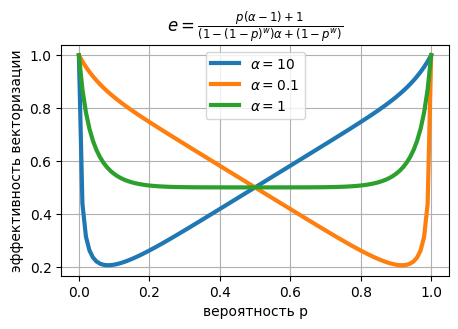
\includegraphics[width=0.45\textwidth]{./pics/text_4_vec_check_mask/chart_e_merged.png}
\end{tabular}
\singlespacing
\caption{Графики зависимостей эффективности векторизации от вероятности перехода $p$ при значениях $\alpha = 10,0$, $\alpha = 0,1$, $\alpha = 1,0$ для слияния двух скалярных блоков без проверки векторной маски (слева) и с проверкой (справа).}
\label{fig:text_4_vec_under_cond_chart_e_merged}
\end{figure}

Приводятся теоретические оценки эффективности векторизации плоского цикла, в котором два скалярных блока (с вероятностями $p$ и $1 - p$ и длинами $\frac{\alpha}{\alpha + 1}$ и $\frac{1}{\alpha + 1}$ соотвественно) сливаются по условию в случае независимости условий из разных итераций плоского цикла.
При этом рассматриваются два варианта векторного кода -- без проверки векторной маски линейного участка на пустоту перед его выполнением и с проверкой (рис.~\ref{fig:text_4_vec_mrg_under_cond_cond}).

Графики зависимостей эффективности векторизаици для разных соотношений длин скалярных блоков приведены на рис.~\ref{fig:text_4_vec_under_cond_chart_e_merged}.
Полученные зависимости показывают низкую эффективность векторизации при слиянии большого количества путей исполнения внутри плоского цикла.

\begin{figure}[ht]
\centering
\begin{tabular}{ll}
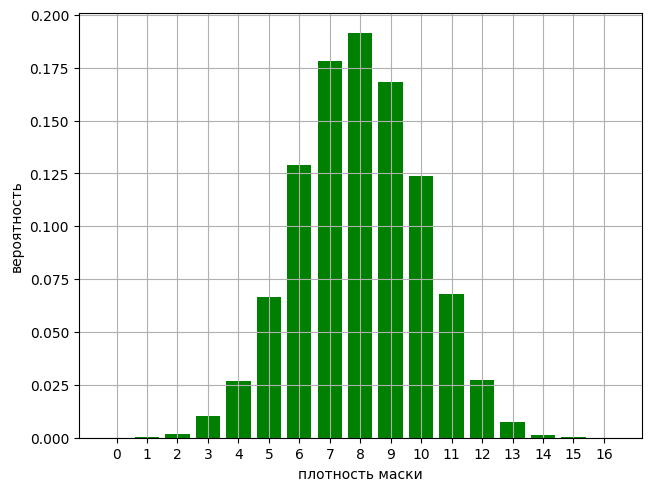
\includegraphics[width=0.45\textwidth]{./pics/text_4_vec_comb_mask/independent_p.png}
&
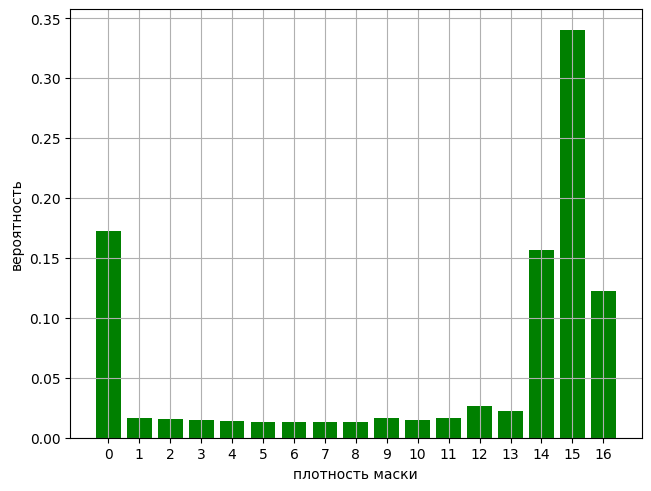
\includegraphics[width=0.45\textwidth]{./pics/text_4_vec_comb_mask/real_p.png}
\end{tabular}
\singlespacing
\caption{Типовая гистограмма распределения плотности векторной маски в предположении независимости условий с разных итераций плоского цикла (слева) и на реальном профиле исполнения (справа).}
\label{fig:text_4_vec_comb_mask_independent_p}
\end{figure}

Отмечается, что проверка векторной маски на пустоту перед выполнением линейного участка зачастую оправдана, так как на реальных приложениях пустые и полные маски встречаются достаточно часто (рис.~\ref{fig:text_4_vec_comb_mask_independent_p}).

%----------------------------------

В п.~4.6 рассматривается подход к повышению плотности масок векторного кода с помощью \textit{объединения масок} и \textit{комбинирования масок} соседних векторных блоков.
Суть объединения векторных масок заключается в следующем.
Если есть два соседних векторных блока \texttt{in\_data\_1} $\rightarrow$ \texttt{block} $\rightarrow$ \texttt{out\_data\_1} и \texttt{in\_data\_2} $\rightarrow$ \texttt{block} $\rightarrow$ \texttt{out\_data\_2}, которые должны выполняться под разными векторными масками \texttt{mask\_1} и \texttt{mask\_2}, и в дополнение к этому для этих масок выполнено условие \texttt{(mask\_1 \& mask\_2) == 0x0} (то есть маски не пересекаются), то вычисление этих двух соседних блоков можно объединить.
Вместо последовательного выполнения двух векторных блоков можно объединить входные данные \texttt{in\_data\_1} и \texttt{in\_data\_2} с помощью слияния \texttt{in\_data = blend(mask\_1, in\_data\_2, in\_data\_1}), после чего выполнить тот же блок вычислений под маской \texttt{mask\_1 | mask\_2}.
Ввиду отсутствия пересечения векторных масок в результирующих выходных данных \texttt{out\_data} будут содержаться как необходимые элементы данных \texttt{out\_data\_1}, так и необходимые элементы данных \texttt{out\_data\_2}.
Последним действием, которое нужно выполнить является извлечение из объединенного результата \texttt{out\_data} данных \texttt{out\_data\_1} и \texttt{out\_data\_2} (рис.~\ref{fig:text_4_vec_comb_mask_comb_masks}).

\begin{figure}[ht]
\centering
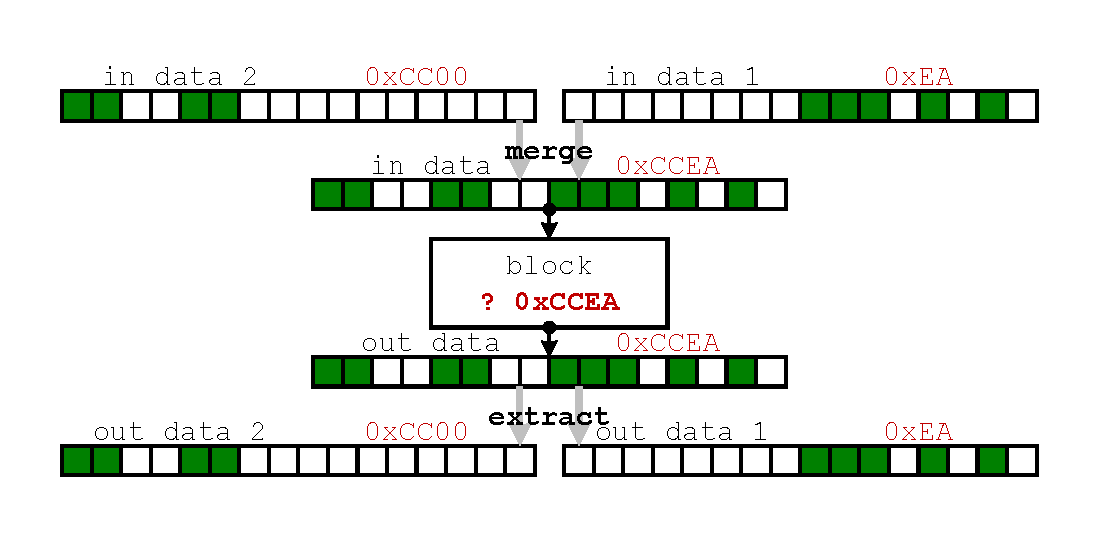
\includegraphics[width=0.8\textwidth]{./pics/text_4_vec_comb_mask/comb_masks.pdf}
\singlespacing
\caption{Схема вычислений с объединением масок двух векторных блоков \texttt{in\_data\_1} $\rightarrow$ \texttt{block} $\rightarrow$ \texttt{out\_data\_1}, \texttt{in\_data\_2} $\rightarrow$ \texttt{block} $\rightarrow$ \texttt{out\_data\_2}}
\label{fig:text_4_vec_comb_mask_comb_masks}
\end{figure}

Комбинирование масок позволяет похожим образом объединить вычисление соседних блоков в случае пересечения векторных масок.
Комбинирование векторных масок рассматривается только теоретически, а для объединения масок поставлен эксперимент для одной из функций точного римановского решателя.
Результаты сравнения эффективнсти векторизации на эмуляторе и на реальной машине при простом слиянии путей исполнения по условию, а также с проверкой векторных масок и с объединением масок представлены на рис.~\ref{fig:text_4_vec_comb_mask_res}.

\begin{figure}[!ht]
\centering
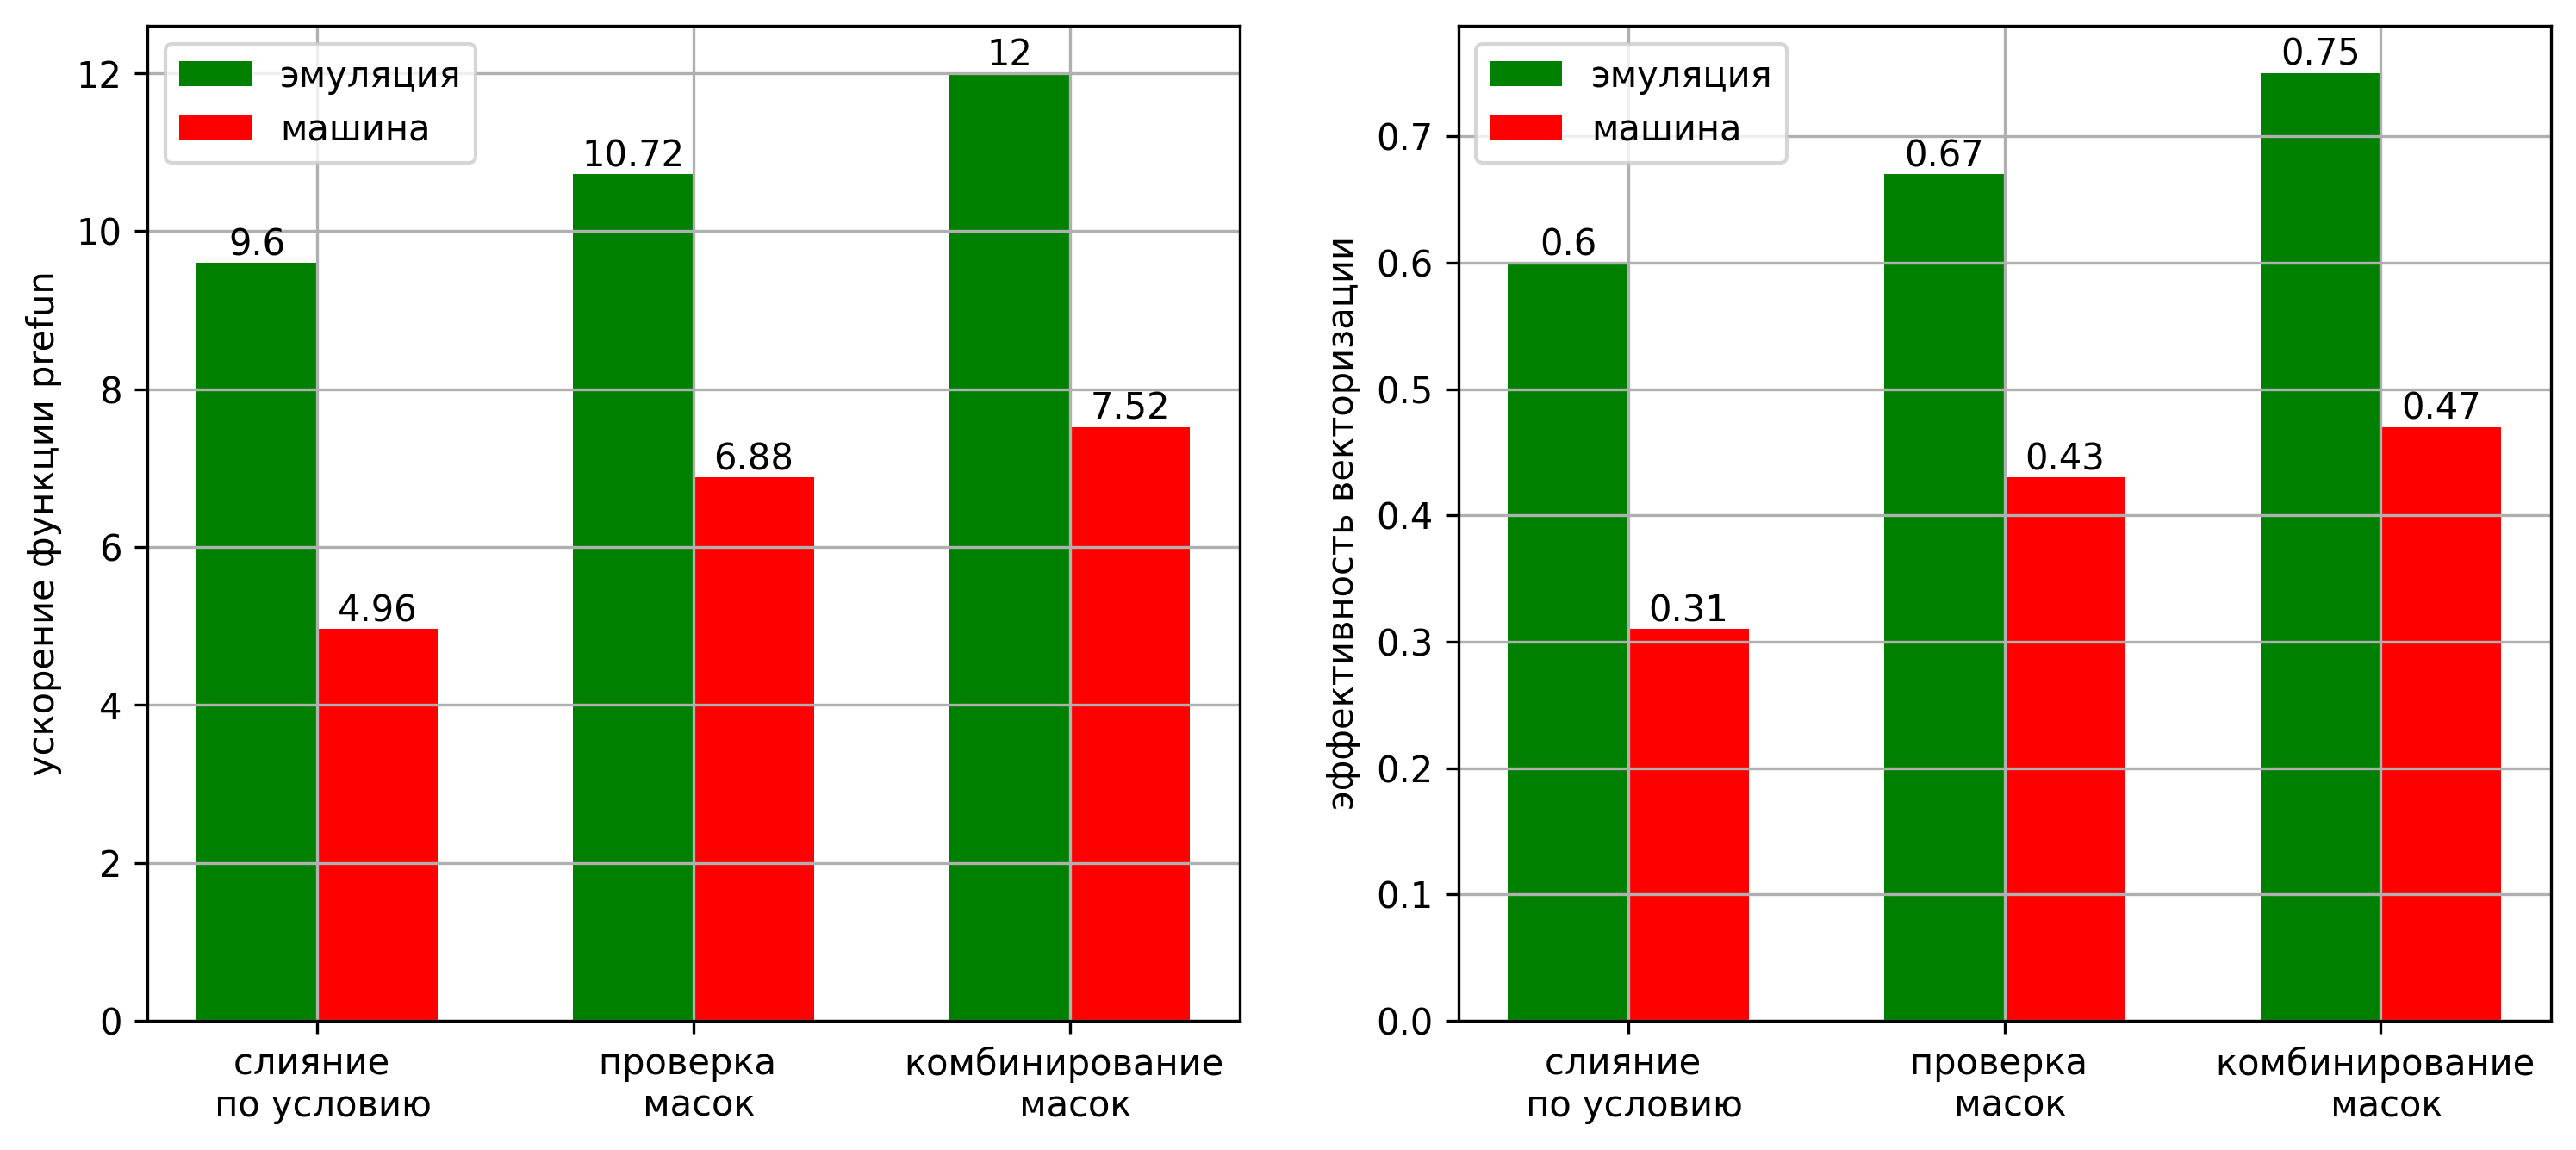
\includegraphics[width=0.8\textwidth]{./pics/text_4_vec_comb_mask/res.png}
\singlespacing
\caption{Результаты сравнения эффективности векторизации при простом слиянии, с проверкой масок и с объединением масок в режимах эмуляции и на реальной машине.}
\label{fig:text_4_vec_comb_mask_res}
\end{figure}

%----------------------------------

В п.~4.7 проводится анализ программного контекста в котором тело плоского цикла само содержит гнезда циклов (рис.~\ref{fig:text_4_vec_flat_loop_vec}).
В этих пунктах отдельно рассматриваются различные виды вложенных циклов, и анализируется влияние этих видов на эффективность векторизации.

\begin{figure}[!ht]
\centering
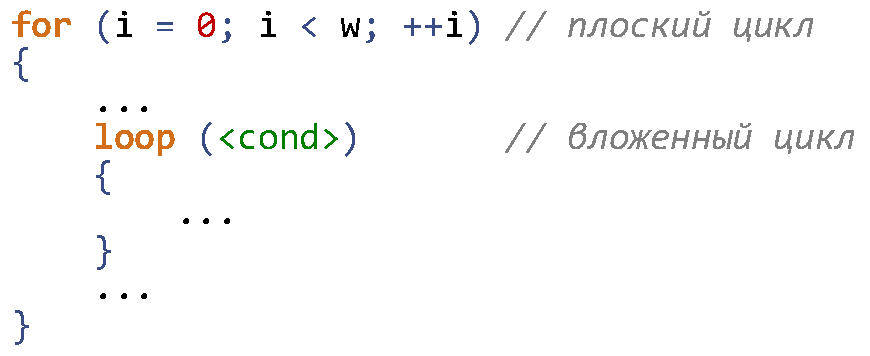
\includegraphics[width=0.6\textwidth]{./pics/text_4_vec_riemann/flat_loop_nest.pdf}
\singlespacing
\caption{Плоский цикл и вложенный в него цикл с произвольным условием выхода.}
\label{fig:text_4_vec_flat_loop_vec}
\end{figure}

В п.~4.7.1 рассматриваются вложенные \textit{циклы с фиксированным количеством итераций}, то есть условие выхода из которого является константным для векторизуемого плоского цикла.
При векторизации такого программного контекста условие выхода из вложенного цикла переносится в векторизованный код в неизменном виде.

\begin{figure}[ht]
\centering
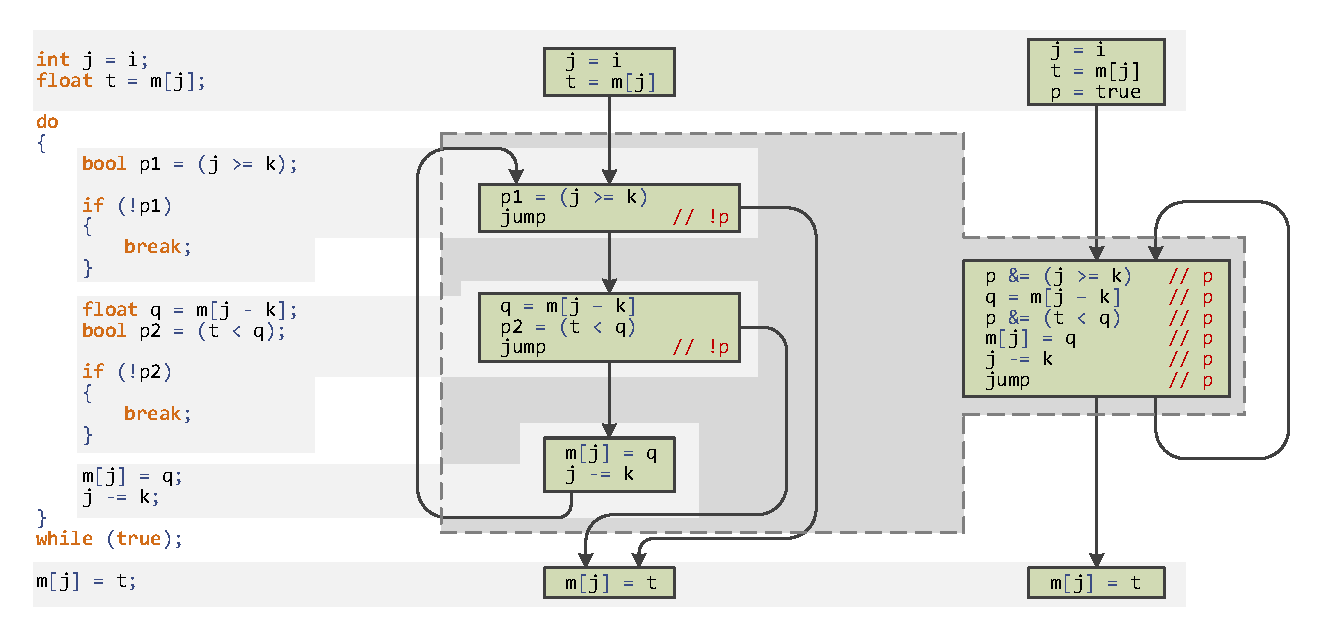
\includegraphics[width=1.0\textwidth]{./pics/text_4_vec_irreg/shell_cfg.pdf}
\singlespacing
\caption{Схема перевода тела вложенного цикла в предикатную форму для последующей векторизации.}
\label{fig:text_4_vec_irreg_shell_cfg}
\end{figure}

В п.~4.7.2 рассматривается вложенный \textit{цикл с непостоянным количеством итераций}, то есть в котором условие выхода из цикла зависит от номера итерации векторизуемого плоского цикла, но изменяется медленно в зависимости от этого номера.
При векторизации такого программного контекста условие выхода из вложенного цикла трансформируется в векторную маску выполнения тела вложенного цикла, и вложенный цикл продолжает исполняться до тех пор, пока эта векторная маска не истощится.
Основной причиной потери производительности при векторизации такого программного контекста является выполнение итераций вложенного цикла под маской низкой плотности.

\begin{figure}[!ht]
\centering
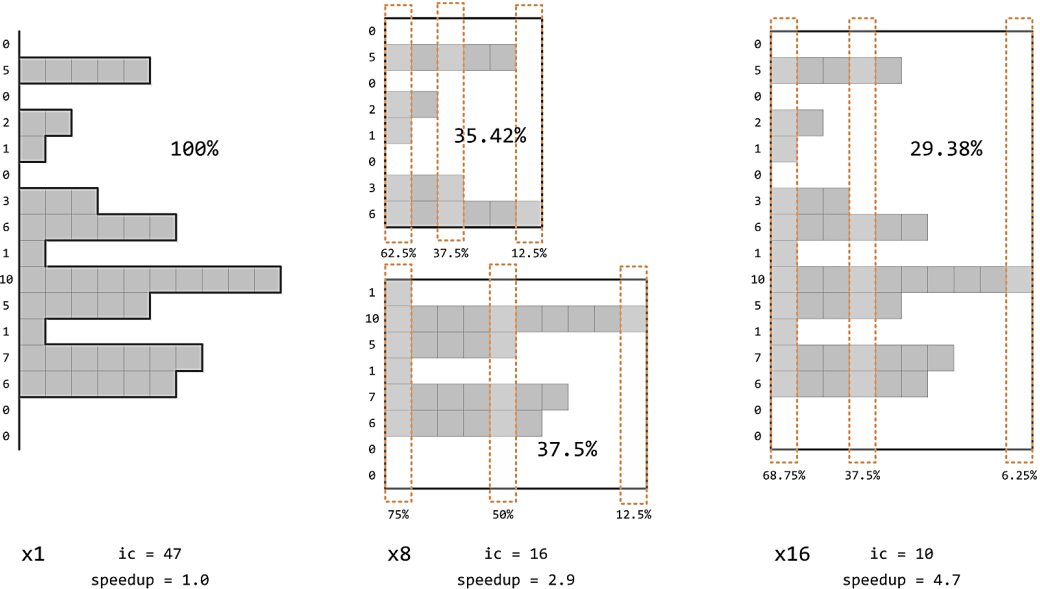
\includegraphics[width=0.6\textwidth]{./pics/text_4_vec_irreg/pack.png}
\singlespacing
\caption{Иллюстрация потери производительности для вложенного цикла с нерегуярным количеством итераций.}
\label{fig:text_4_vec_irreg_pack}
\end{figure}

\begin{figure}[!ht]
\centering
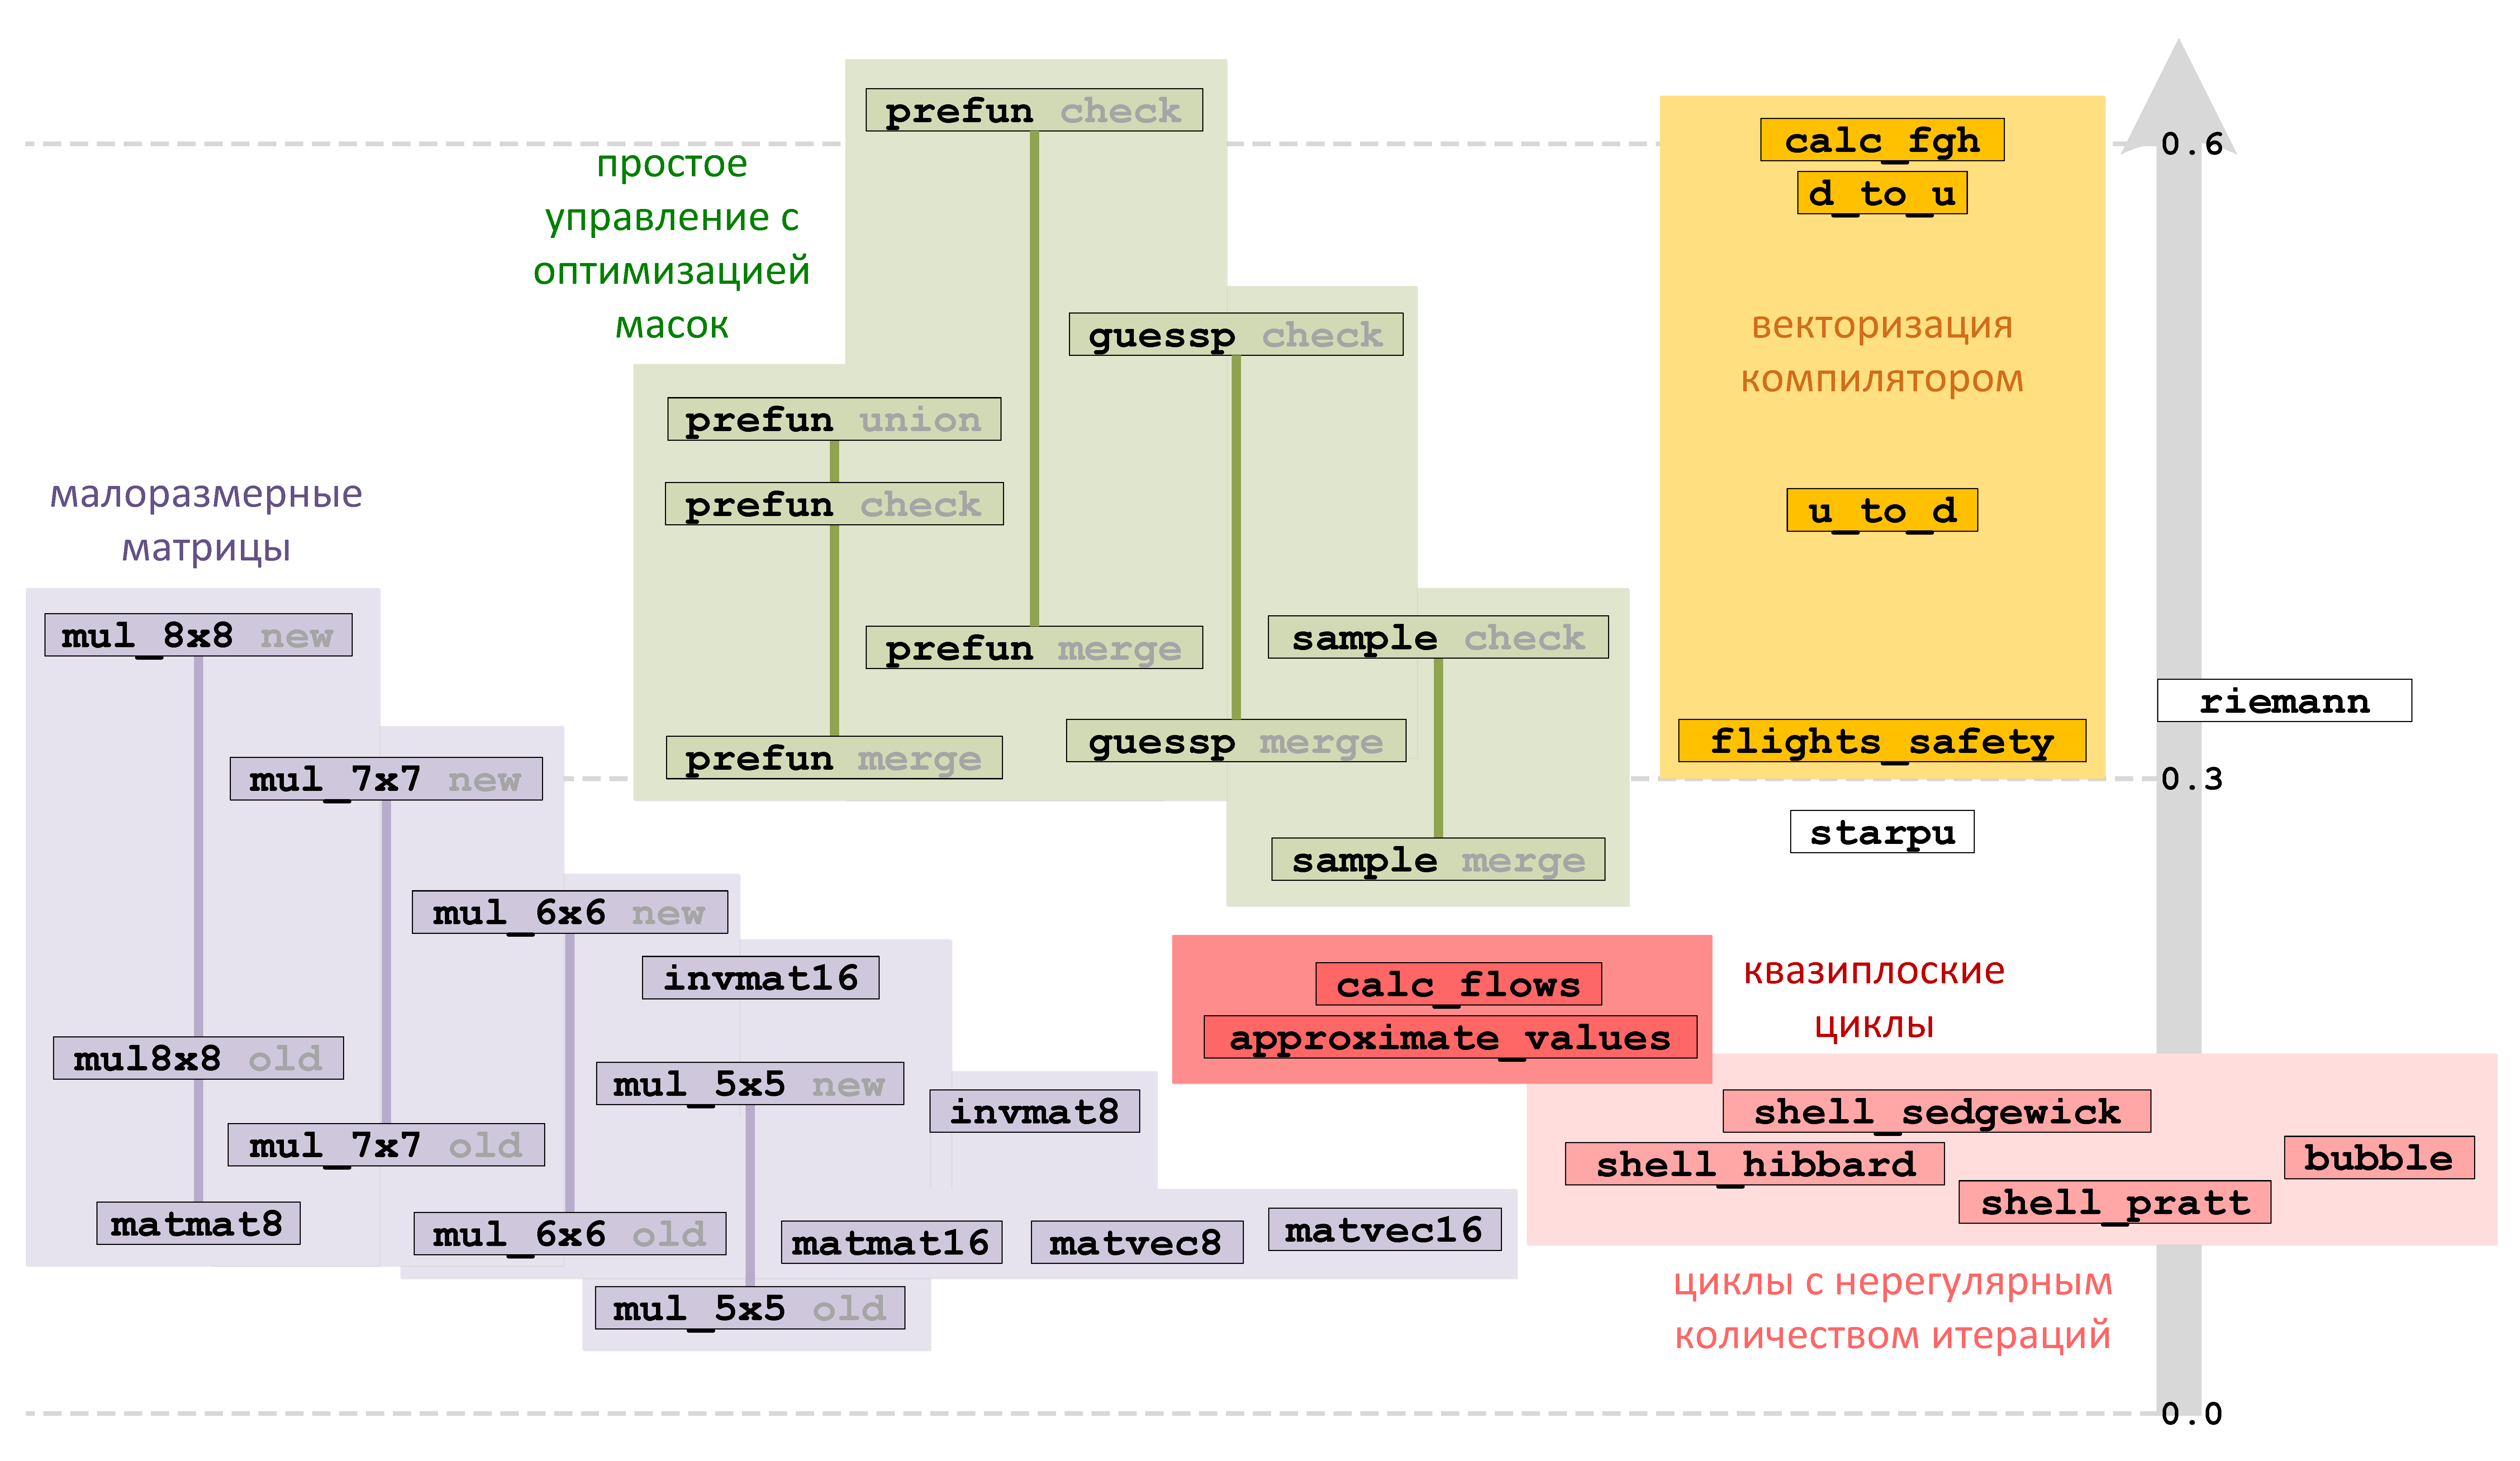
\includegraphics[width=1.0\textwidth]{./pics/text_4_fin/map_cut.pdf}
\singlespacing
\caption{Карта эффективности векторизации.}
\label{fig:text_4_fin_map}
\end{figure}

В п.~4.7.3 и п.~4.7.4 рассматривается вещественный и целочисленный программный контекст в котором вложенный цикл характеризуется как \textit{цикл с нерегулярным количеством итераций}, то есть условие выхода из вложенного цикла не только не зависит от номера итерации плоского цикла, но эта зависимость носит стохастический характер.
При векторизации такого программного контекста плотность маски выполнения вложенного цикла является крайне низкой, что приводит к наиболее серьезной потери производительности (рис.~\ref{fig:text_4_vec_irreg_pack}). 

%----------------------------------

В выводах из главы приводится общая карта рассмотренного в главе векторизованного программного контекста, представленная на рис.~\ref{fig:text_4_fin_map}.

Из карты делается вывод, что наиболее неудобным программным контекстом для векторизации являются гнезда циклов с нерегулярным количеством итераций, а также \textit{квазиплоские циклы}, то есть циклы, нарушающие некоторые требования, предъявляеимые к плоским циклам (дополнительная косвенность при обращении в память, невыровненность данных и другие).
Наиболее удобным контекстом для векторизации являются плоские циклы с простым управлением и применением проверок и объединения масок.

%---------------------------------------------------------------------------------------------------

\section*{Список основных публикаций автора по теме работы}

\begin{enumerate}
\item Рыбаков А. А. Декомпозиция расчетной сетки с помощью генетического алгоритма. // Программные продукты и системы, 2025, 38(2), С. 337-344.
\item Рыбаков А. А. Векторизация циклов с условными операциями с помощью комбинирования векторных масок. // Современные информационные технологии и ИТ-образование, 2024, Т. 20, № 3, с. 520-534.
\item Гуличева А. А., Рыбаков А. А. Реберная раскраска кубического графа в задаче распараллелирования расчетов на неструктурированной поверхностной расчетной сетке. // Программные продукты и системы, 2024, 37(3), С. 374-383.
\item Рыбаков А. А., Швиндт А. Н. Создание инструментария для векторизации тела плоского цикла с помощью векторных инструкций AVX-512. // Программные продукты и системы, 2023, Т. 36, № 4, с. 561-572.
\item Рыбаков А. А. Геометрическое перестроение расчетной сетки с помощью общей огибающей семейства сфер в задаче ледообразования. // Современные информационные технологии и ИТ-образование, 2023, Т. 19, № 2, с. 282-291.
\item Рыбаков А. А., Мещеряков А. О. Векторизация трехмерного метода погруженных границ для повышения эффективности расчетов на микропроцессорах Intel. // Программные продукты и системы, 2023, Т. 36, № 1, с. 130-143.
\item Meshcheryakov A. O., Rybakov A. A. Evolution of the surface computational mesh in the ice accretion process. // Lobachevskii Journal of Mathematics, 2023, Vol. 44, No. 11, p. 361-378.
\item Freylekhman S. A., Rybakov A. A. Self-intersection elimination for unstructured surface computational meshes. // Lobachevskii Journal of Mathematics, 2022, Vol. 43, No. 10, p. 2846-2852.
\item Рыбаков А. А. Векторизация программного кода, содержащего маловероятные регионы, в задачах вычислительной геометрии. // Современные информационные технологии и ИТ-образование, 2022, Т. 18, № 1, с. 28-38.
\item Багров А. Д., Рыбаков А. А. Сглаживание границ между доменами поверхностной расчетной сетки. // Современные информационные технологии и ИТ-образование, 2021, Т. 17, № 2, с. 265-274.
\item Shabanov B. M., Rybakov A. A., Shumilin S. S., Vorobyov M. Yu. Scaling of supercomputer calculations on unstructered surface computational meshes. // Lobachevskii Journal of Mathematics, 2021, Vol. 42, No. 11, p. 2571-2579.
\item Шабанов Б. М., Рыбаков А. А., Чопорняк А. Д. Оптимизации, применяемые к графу потока управления программы для повышения эффективности векторизации плоских циклов. // Труды НИИСИ РАН, 2021, Т. 11, № 2, с. 11-19.
\item Рыбаков А. А., Чопорняк А. Д. Декомпозиция поверхностной неструктурированной расчетной сетки для масштабирования вычислений на суперкомпьютере. // Современные информационные технологии и ИТ-образование, 2020, Т. 16, № 4, с. 851-861.
\item Воробьев М. Ю., Рыбаков А. А., Никсон Муганда Очара. Исследование масштабируемости плотных параллельных вычислений на микропроцессорах Intel. // Инжиниринг предприятий и управление знаниями (ИП\&УЗ-2020). Сборник научных трудов XXIII Международной научной конференции, 2020, с. 45-52.
\item Рыбаков А. А. Метод погруженной границы с использованием фиктивных ячеек в трехмерной постановке. // Современные информационные технологии и ИТ-образование, 2020, Т. 16, № 2, с. 321-330.
\item Savin G. I., Shabanov B. M., Rybakov A. A., Shumilin S. S. Vectorization of flat loops of arbitrary structure using instructions AVX-512. // Lobachevskii Journal of Mathematics, 2020, Vol. 41, No. 12, p. 2566-2574.
\item Воробьев М. Ю., Рыбаков А. А., Чопорняк А. Д. Сравнение стратегий распараллеливания векторизованного римановского решателя с помощью OpenMP для микропроцессора Intel Xeon Phi KNL. // Труды НИИСИ РАН, 2020, Т. 10, № 5-6, с. 113-119.
\item Рыбаков А. А., Чопорняк А. Д. Повышение производительности векторного кода с помощью мониторинга плотности масок в векторных инструкциях. // Труды НИИСИ РАН, 2020, Т. 10, № 4, с. 40-47.
\item Рыбаков А. А. Векторизация нахождения пересечения объемной и поверхностной сеток для микропроцессоров с поддержкой AVX-512. // Труды НИИСИ РАН, 2019, Т. 9, № 5, с. 5-14.
\item Рыбаков А. А., Шумилин С. С. Исследование эффективности векторизации гнезд циклов с нерегулярным числом итераций. // Программные системы: Теория и алгоритмы, 2019, Т. 10, № 4 (43), с. 77-96.
\item Rybakov A. A., Shumilin S. S. Vectorization of the Riemann solver using the AVX-512 instruction set. // Program Systems: Theory and Applications, 2019, Vol. 10, № 3 (42), p. 41-58.
\item Рыбаков А. А., Шумилин С. С. Векторизация римановского решателя с использованием набора инструкций AVX-512. // Программные системы: Теория и приложения, 2019, Т. 10, № 3 (42), с. 59-80.
\item Rybakov A. A., Shumilin S. S. Approximate methods of the surface mesh deformation in two-dimensional cases. // Lobachevskii Journal of Mathematics, 2019, Vol. 40, No. 11, p. 1848-1852.
\item Savin G. I., Benderskiy L. A., Lyubimov D. A., Rybakov A. A. RANS/ILES method optimization for effective calculations on supercomputer. // Lobachevskii Journal of Mathematics, 2019, Vol. 40, No. 5, p. 566-573.
\item Shabanov B. M., Rybakov A. A., Shumilin S. S. Vectorization of high-performance scientific calculations using AVX-512 instruction set. // Lobachevskii Journal of Mathematics, 2019, Vol. 40, No. 5, p. 580-598.
\item Бендерский Л. А., Рыбаков А. А., Шумилин С. С. Векторизация перемножения малоразмерных матриц специального вида с использованием инструкций AVX-512. // Современные информационные технологии и ИТ-образование, 2018, Т. 14, № 3, с. 594-602.
\item Рыбаков А. А., Шумилин С. С. Векторизация сильно разветвленного управления с помощью инструкций AVX-512. // Труды НИИСИ РАН, 2018, Т. 8, № 4, с. 114-126.
\item Бендерский Л. А., Любимов Д. А., Рыбаков А. А. Инструментарий подготовки блочно-структурированной сетки для проведения расчетов методом RANS/ILES. // Труды НИИСИ РАН, 2018, Т. 8, № 4, с. 102-106.
\item Рыбаков А. А., Телегин П. Н., Шабанов Б. М. Проблемы векторизации гнезд циклов с использованием инструкций AVX-512. // Электронный научный журнал: Программные продукты, системы и алгоритмы, 2018, № 3, с. 1-11.
\item Бендерский Л. А., Лещев С. А., Рыбаков А. А. Векторизация операций над матрицами малой размерности для процессора Intel Xeon Phi Knights Landing. // Современные информационные технологии и ИТ-образование, 2018, Т. 14, № 1, с. 73-90.
\item Рыбаков А. А. Распределение вычислительной нагрузки между узлами гетерогенного вычислительного кластера. // Электронный научный журнал: Программные продукты, системы и алгоритмы, 2018, № 1, с. 26-32.
\item Бендерский Л. А., Любимов Д. А., Рыбаков А. А. Анализ эффективности масштабирования при расчетах высокоскоростных турбулентных течений на суперкомпьютере RANS/ILES методом высокого разрешения. // Труды НИИСИ РАН, 2017, Т. 7, № 4, с. 32-40.
\item Рыбаков А. А. Оптимизация задачи об определении конфликтов с опасными зонами движения летательных аппаратов для выполнения на Intel Xeon Phi. // Программные продукты и системы, 2017, Т. 30, №3, с. 524-528.
\item Рыбаков А. А. Внутреннее представление и механизм межпроцессного обмена для блочно-структурированной сетки при выполнении расчетов на суперкомпьютере. // Программные системы: теория и приложения, 2017, № 8:1 (32), с. 121-134.
\item Рыбаков А. А. Распределение вычислительной нагрузки между узлами суперкомпьютерного кластера при расчетах задач газовой динамики с дроблением расчетной сетки. // Современные информационные технологии и ИТ-образование, 2016, Т. 12, № 2, с. 101-107.
\end{enumerate}

\end{document}
